\documentclass[twoside]{book}

% Packages required by doxygen
\usepackage{calc}
\usepackage{doxygen}
\usepackage{graphicx}
\usepackage[utf8]{inputenc}
\usepackage{makeidx}
\usepackage{multicol}
\usepackage{multirow}
\usepackage{fixltx2e}
\PassOptionsToPackage{warn}{textcomp}
\usepackage{textcomp}
\usepackage[nointegrals]{wasysym}
\usepackage[table]{xcolor}

% Font selection
\usepackage[T1]{fontenc}
\usepackage{mathptmx}
\usepackage[scaled=.90]{helvet}
\usepackage{courier}
\usepackage{amssymb}
\usepackage{sectsty}
\renewcommand{\familydefault}{\sfdefault}
\allsectionsfont{%
  \fontseries{bc}\selectfont%
  \color{darkgray}%
}
\renewcommand{\DoxyLabelFont}{%
  \fontseries{bc}\selectfont%
  \color{darkgray}%
}
\newcommand{\+}{\discretionary{\mbox{\scriptsize$\hookleftarrow$}}{}{}}

% Page & text layout
\usepackage{geometry}
\geometry{%
  a4paper,%
  top=2.5cm,%
  bottom=2.5cm,%
  left=2.5cm,%
  right=2.5cm%
}
\tolerance=750
\hfuzz=15pt
\hbadness=750
\setlength{\emergencystretch}{15pt}
\setlength{\parindent}{0cm}
\setlength{\parskip}{0.2cm}
\makeatletter
\renewcommand{\paragraph}{%
  \@startsection{paragraph}{4}{0ex}{-1.0ex}{1.0ex}{%
    \normalfont\normalsize\bfseries\SS@parafont%
  }%
}
\renewcommand{\subparagraph}{%
  \@startsection{subparagraph}{5}{0ex}{-1.0ex}{1.0ex}{%
    \normalfont\normalsize\bfseries\SS@subparafont%
  }%
}
\makeatother

% Headers & footers
\usepackage{fancyhdr}
\pagestyle{fancyplain}
\fancyhead[LE]{\fancyplain{}{\bfseries\thepage}}
\fancyhead[CE]{\fancyplain{}{}}
\fancyhead[RE]{\fancyplain{}{\bfseries\leftmark}}
\fancyhead[LO]{\fancyplain{}{\bfseries\rightmark}}
\fancyhead[CO]{\fancyplain{}{}}
\fancyhead[RO]{\fancyplain{}{\bfseries\thepage}}
\fancyfoot[LE]{\fancyplain{}{}}
\fancyfoot[CE]{\fancyplain{}{}}
\fancyfoot[RE]{\fancyplain{}{\bfseries\scriptsize 2014年08月21日(木) 17時11分53秒作成 -\/ My Project / 構成\+:  Doxygen }}
\fancyfoot[LO]{\fancyplain{}{\bfseries\scriptsize 2014年08月21日(木) 17時11分53秒作成 -\/ My Project / 構成\+:  Doxygen }}
\fancyfoot[CO]{\fancyplain{}{}}
\fancyfoot[RO]{\fancyplain{}{}}
\renewcommand{\footrulewidth}{0.4pt}
\renewcommand{\chaptermark}[1]{%
  \markboth{#1}{}%
}
\renewcommand{\sectionmark}[1]{%
  \markright{\thesection\ #1}%
}

% Indices & bibliography
\usepackage{natbib}
\usepackage[titles]{tocloft}
\setcounter{tocdepth}{3}
\setcounter{secnumdepth}{5}
\makeindex

% Hyperlinks (required, but should be loaded last)
\usepackage{ifpdf}
\ifpdf
  \usepackage[pdftex,pagebackref=true]{hyperref}
\else
  \usepackage[ps2pdf,pagebackref=true]{hyperref}
\fi
\hypersetup{%
  colorlinks=true,%
  linkcolor=blue,%
  citecolor=blue,%
  unicode%
}

% Custom commands
\newcommand{\clearemptydoublepage}{%
  \newpage{\pagestyle{empty}\cleardoublepage}%
}


%===== C O N T E N T S =====

\begin{document}

% Titlepage & ToC
\hypersetup{pageanchor=false,
             bookmarks=true,
             bookmarksnumbered=true,
             pdfencoding=unicode
            }
\pagenumbering{roman}
\begin{titlepage}
\vspace*{7cm}
\begin{center}%
{\Large My Project }\\
\vspace*{1cm}
{\large 構築\+: Doxygen 1.8.7}\\
\vspace*{0.5cm}
{\small 2014年08月21日(木) 17時11分53秒}\\
\end{center}
\end{titlepage}
\clearemptydoublepage
\tableofcontents
\clearemptydoublepage
\pagenumbering{arabic}
\hypersetup{pageanchor=true}

%--- Begin generated contents ---
\chapter{階層索引}
\section{クラス階層}
クラス階層一覧です。大雑把に文字符号順で並べられています。\begin{DoxyCompactList}
\item \contentsline{section}{A\+Object}{\pageref{class_a_object}}{}
\begin{DoxyCompactList}
\item \contentsline{section}{Bullet}{\pageref{class_bullet}}{}
\begin{DoxyCompactList}
\item \contentsline{section}{Aim\+Bullet}{\pageref{class_aim_bullet}}{}
\item \contentsline{section}{Normal\+Bullet}{\pageref{class_normal_bullet}}{}
\end{DoxyCompactList}
\item \contentsline{section}{Character}{\pageref{class_character}}{}
\begin{DoxyCompactList}
\item \contentsline{section}{Enemy}{\pageref{class_enemy}}{}
\begin{DoxyCompactList}
\item \contentsline{section}{Jump\+Kame}{\pageref{class_jump_kame}}{}
\item \contentsline{section}{Kame}{\pageref{class_kame}}{}
\end{DoxyCompactList}
\item \contentsline{section}{Player}{\pageref{class_player}}{}
\end{DoxyCompactList}
\item \contentsline{section}{Item}{\pageref{class_item}}{}
\begin{DoxyCompactList}
\item \contentsline{section}{Coin}{\pageref{class_coin}}{}
\item \contentsline{section}{Goal\+Flag}{\pageref{class_goal_flag}}{}
\end{DoxyCompactList}
\end{DoxyCompactList}
\item \contentsline{section}{Attack}{\pageref{class_attack}}{}
\begin{DoxyCompactList}
\item \contentsline{section}{Aim\+Attack}{\pageref{class_aim_attack}}{}
\item \contentsline{section}{No\+Attack}{\pageref{class_no_attack}}{}
\item \contentsline{section}{Normal\+Attack}{\pageref{class_normal_attack}}{}
\end{DoxyCompactList}
\item \contentsline{section}{Character\+Controller}{\pageref{class_character_controller}}{}
\begin{DoxyCompactList}
\item \contentsline{section}{Jump\+Enemy}{\pageref{class_jump_enemy}}{}
\item \contentsline{section}{Player\+Controller}{\pageref{class_player_controller}}{}
\item \contentsline{section}{Walk\+Straight}{\pageref{class_walk_straight}}{}
\end{DoxyCompactList}
\item \contentsline{section}{Field}{\pageref{class_field}}{}
\item \contentsline{section}{Game\+Main}{\pageref{class_game_main}}{}
\item \contentsline{section}{Load\+Graphic}{\pageref{class_load_graphic}}{}
\item \contentsline{section}{Map}{\pageref{class_map}}{}
\item \contentsline{section}{Map\+Factory}{\pageref{class_map_factory}}{}
\item \contentsline{section}{Menu}{\pageref{class_menu}}{}
\item \contentsline{section}{Menu\+:\+:Menu\+Element\+\_\+t}{\pageref{struct_menu_1_1_menu_element__t}}{}
\item \contentsline{section}{Object\+Manager}{\pageref{class_object_manager}}{}
\item \contentsline{section}{Two\+Dimension}{\pageref{struct_two_dimension}}{}
\end{DoxyCompactList}

\chapter{クラス索引}
\section{クラス一覧}
クラス・構造体・共用体・インターフェースの一覧です。\begin{DoxyCompactList}
\item\contentsline{section}{\hyperlink{class_aim_attack}{Aim\+Attack} }{\pageref{class_aim_attack}}{}
\item\contentsline{section}{\hyperlink{class_aim_bullet}{Aim\+Bullet} }{\pageref{class_aim_bullet}}{}
\item\contentsline{section}{\hyperlink{class_a_object}{A\+Object} }{\pageref{class_a_object}}{}
\item\contentsline{section}{\hyperlink{class_attack}{Attack} }{\pageref{class_attack}}{}
\item\contentsline{section}{\hyperlink{class_bullet}{Bullet} }{\pageref{class_bullet}}{}
\item\contentsline{section}{\hyperlink{class_character}{Character} }{\pageref{class_character}}{}
\item\contentsline{section}{\hyperlink{class_character_controller}{Character\+Controller} }{\pageref{class_character_controller}}{}
\item\contentsline{section}{\hyperlink{class_coin}{Coin} }{\pageref{class_coin}}{}
\item\contentsline{section}{\hyperlink{class_enemy}{Enemy} }{\pageref{class_enemy}}{}
\item\contentsline{section}{\hyperlink{class_field}{Field} }{\pageref{class_field}}{}
\item\contentsline{section}{\hyperlink{class_game_main}{Game\+Main} }{\pageref{class_game_main}}{}
\item\contentsline{section}{\hyperlink{class_goal_flag}{Goal\+Flag} }{\pageref{class_goal_flag}}{}
\item\contentsline{section}{\hyperlink{class_item}{Item} }{\pageref{class_item}}{}
\item\contentsline{section}{\hyperlink{class_jump_enemy}{Jump\+Enemy} }{\pageref{class_jump_enemy}}{}
\item\contentsline{section}{\hyperlink{class_jump_kame}{Jump\+Kame} }{\pageref{class_jump_kame}}{}
\item\contentsline{section}{\hyperlink{class_kame}{Kame} }{\pageref{class_kame}}{}
\item\contentsline{section}{\hyperlink{class_load_graphic}{Load\+Graphic} }{\pageref{class_load_graphic}}{}
\item\contentsline{section}{\hyperlink{class_map}{Map} }{\pageref{class_map}}{}
\item\contentsline{section}{\hyperlink{class_map_factory}{Map\+Factory} }{\pageref{class_map_factory}}{}
\item\contentsline{section}{\hyperlink{class_menu}{Menu} }{\pageref{class_menu}}{}
\item\contentsline{section}{\hyperlink{struct_menu_1_1_menu_element__t}{Menu\+::\+Menu\+Element\+\_\+t} }{\pageref{struct_menu_1_1_menu_element__t}}{}
\item\contentsline{section}{\hyperlink{class_no_attack}{No\+Attack} }{\pageref{class_no_attack}}{}
\item\contentsline{section}{\hyperlink{class_normal_attack}{Normal\+Attack} }{\pageref{class_normal_attack}}{}
\item\contentsline{section}{\hyperlink{class_normal_bullet}{Normal\+Bullet} }{\pageref{class_normal_bullet}}{}
\item\contentsline{section}{\hyperlink{class_object_manager}{Object\+Manager} }{\pageref{class_object_manager}}{}
\item\contentsline{section}{\hyperlink{class_player}{Player} }{\pageref{class_player}}{}
\item\contentsline{section}{\hyperlink{class_player_controller}{Player\+Controller} }{\pageref{class_player_controller}}{}
\item\contentsline{section}{\hyperlink{struct_two_dimension}{Two\+Dimension} }{\pageref{struct_two_dimension}}{}
\item\contentsline{section}{\hyperlink{class_walk_straight}{Walk\+Straight} }{\pageref{class_walk_straight}}{}
\end{DoxyCompactList}

\chapter{ファイル索引}
\section{ファイル一覧}
ファイル一覧です。\begin{DoxyCompactList}
\item\contentsline{section}{\hyperlink{_aim_attack_8cpp}{Aim\+Attack.\+cpp} }{\pageref{_aim_attack_8cpp}}{}
\item\contentsline{section}{\hyperlink{_aim_attack_8h}{Aim\+Attack.\+h} }{\pageref{_aim_attack_8h}}{}
\item\contentsline{section}{\hyperlink{_aim_bullet_8cpp}{Aim\+Bullet.\+cpp} }{\pageref{_aim_bullet_8cpp}}{}
\item\contentsline{section}{\hyperlink{_aim_bullet_8h}{Aim\+Bullet.\+h} }{\pageref{_aim_bullet_8h}}{}
\item\contentsline{section}{\hyperlink{_a_object_8cpp}{A\+Object.\+cpp} }{\pageref{_a_object_8cpp}}{}
\item\contentsline{section}{\hyperlink{_a_object_8h}{A\+Object.\+h} }{\pageref{_a_object_8h}}{}
\item\contentsline{section}{\hyperlink{_attack_8cpp}{Attack.\+cpp} }{\pageref{_attack_8cpp}}{}
\item\contentsline{section}{\hyperlink{_attack_8h}{Attack.\+h} }{\pageref{_attack_8h}}{}
\item\contentsline{section}{\hyperlink{_bullet_8cpp}{Bullet.\+cpp} }{\pageref{_bullet_8cpp}}{}
\item\contentsline{section}{\hyperlink{_bullet_8h}{Bullet.\+h} }{\pageref{_bullet_8h}}{}
\item\contentsline{section}{\hyperlink{_character_8cpp}{Character.\+cpp} }{\pageref{_character_8cpp}}{}
\item\contentsline{section}{\hyperlink{_character_8h}{Character.\+h} }{\pageref{_character_8h}}{}
\item\contentsline{section}{\hyperlink{_character_controller_8cpp}{Character\+Controller.\+cpp} }{\pageref{_character_controller_8cpp}}{}
\item\contentsline{section}{\hyperlink{_character_controller_8h}{Character\+Controller.\+h} }{\pageref{_character_controller_8h}}{}
\item\contentsline{section}{\hyperlink{_coin_8cpp}{Coin.\+cpp} }{\pageref{_coin_8cpp}}{}
\item\contentsline{section}{\hyperlink{_coin_8h}{Coin.\+h} }{\pageref{_coin_8h}}{}
\item\contentsline{section}{\hyperlink{_enemy_8cpp}{Enemy.\+cpp} }{\pageref{_enemy_8cpp}}{}
\item\contentsline{section}{\hyperlink{_enemy_8h}{Enemy.\+h} }{\pageref{_enemy_8h}}{}
\item\contentsline{section}{\hyperlink{_field_8cpp}{Field.\+cpp} }{\pageref{_field_8cpp}}{}
\item\contentsline{section}{\hyperlink{_field_8h}{Field.\+h} }{\pageref{_field_8h}}{}
\item\contentsline{section}{\hyperlink{_game_main_8cpp}{Game\+Main.\+cpp} }{\pageref{_game_main_8cpp}}{}
\item\contentsline{section}{\hyperlink{_game_main_8h}{Game\+Main.\+h} }{\pageref{_game_main_8h}}{}
\item\contentsline{section}{\hyperlink{_goal_flag_8cpp}{Goal\+Flag.\+cpp} }{\pageref{_goal_flag_8cpp}}{}
\item\contentsline{section}{\hyperlink{_goal_flag_8h}{Goal\+Flag.\+h} }{\pageref{_goal_flag_8h}}{}
\item\contentsline{section}{\hyperlink{_item_8cpp}{Item.\+cpp} }{\pageref{_item_8cpp}}{}
\item\contentsline{section}{\hyperlink{_item_8h}{Item.\+h} }{\pageref{_item_8h}}{}
\item\contentsline{section}{\hyperlink{_jump_enemy_8cpp}{Jump\+Enemy.\+cpp} }{\pageref{_jump_enemy_8cpp}}{}
\item\contentsline{section}{\hyperlink{_jump_enemy_8h}{Jump\+Enemy.\+h} }{\pageref{_jump_enemy_8h}}{}
\item\contentsline{section}{\hyperlink{_jump_kame_8cpp}{Jump\+Kame.\+cpp} }{\pageref{_jump_kame_8cpp}}{}
\item\contentsline{section}{\hyperlink{_jump_kame_8h}{Jump\+Kame.\+h} }{\pageref{_jump_kame_8h}}{}
\item\contentsline{section}{\hyperlink{_kame_8cpp}{Kame.\+cpp} }{\pageref{_kame_8cpp}}{}
\item\contentsline{section}{\hyperlink{_kame_8h}{Kame.\+h} }{\pageref{_kame_8h}}{}
\item\contentsline{section}{\hyperlink{_load_graphic_8cpp}{Load\+Graphic.\+cpp} }{\pageref{_load_graphic_8cpp}}{}
\item\contentsline{section}{\hyperlink{_load_graphic_8h}{Load\+Graphic.\+h} }{\pageref{_load_graphic_8h}}{}
\item\contentsline{section}{\hyperlink{main_8cpp}{main.\+cpp} }{\pageref{main_8cpp}}{}
\item\contentsline{section}{\hyperlink{_map_8cpp}{Map.\+cpp} }{\pageref{_map_8cpp}}{}
\item\contentsline{section}{\hyperlink{_map_8h}{Map.\+h} }{\pageref{_map_8h}}{}
\item\contentsline{section}{\hyperlink{_map_factory_8cpp}{Map\+Factory.\+cpp} }{\pageref{_map_factory_8cpp}}{}
\item\contentsline{section}{\hyperlink{_map_factory_8h}{Map\+Factory.\+h} }{\pageref{_map_factory_8h}}{}
\item\contentsline{section}{\hyperlink{_menu_8cpp}{Menu.\+cpp} }{\pageref{_menu_8cpp}}{}
\item\contentsline{section}{\hyperlink{_menu_8h}{Menu.\+h} }{\pageref{_menu_8h}}{}
\item\contentsline{section}{\hyperlink{_no_attack_8cpp}{No\+Attack.\+cpp} }{\pageref{_no_attack_8cpp}}{}
\item\contentsline{section}{\hyperlink{_no_attack_8h}{No\+Attack.\+h} }{\pageref{_no_attack_8h}}{}
\item\contentsline{section}{\hyperlink{_normal_attack_8cpp}{Normal\+Attack.\+cpp} }{\pageref{_normal_attack_8cpp}}{}
\item\contentsline{section}{\hyperlink{_normal_attack_8h}{Normal\+Attack.\+h} }{\pageref{_normal_attack_8h}}{}
\item\contentsline{section}{\hyperlink{_normal_bullet_8cpp}{Normal\+Bullet.\+cpp} }{\pageref{_normal_bullet_8cpp}}{}
\item\contentsline{section}{\hyperlink{_normal_bullet_8h}{Normal\+Bullet.\+h} }{\pageref{_normal_bullet_8h}}{}
\item\contentsline{section}{\hyperlink{_object_manager_8cpp}{Object\+Manager.\+cpp} }{\pageref{_object_manager_8cpp}}{}
\item\contentsline{section}{\hyperlink{_object_manager_8h}{Object\+Manager.\+h} }{\pageref{_object_manager_8h}}{}
\item\contentsline{section}{\hyperlink{_player_8cpp}{Player.\+cpp} }{\pageref{_player_8cpp}}{}
\item\contentsline{section}{\hyperlink{_player_8h}{Player.\+h} }{\pageref{_player_8h}}{}
\item\contentsline{section}{\hyperlink{_player_controller_8cpp}{Player\+Controller.\+cpp} }{\pageref{_player_controller_8cpp}}{}
\item\contentsline{section}{\hyperlink{_player_controller_8h}{Player\+Controller.\+h} }{\pageref{_player_controller_8h}}{}
\item\contentsline{section}{\hyperlink{_walk_straight_8cpp}{Walk\+Straight.\+cpp} }{\pageref{_walk_straight_8cpp}}{}
\item\contentsline{section}{\hyperlink{_walk_straight_8h}{Walk\+Straight.\+h} }{\pageref{_walk_straight_8h}}{}
\end{DoxyCompactList}

\chapter{クラス詳解}
\hypertarget{class_aim_attack}{\section{Aim\+Attack クラス}
\label{class_aim_attack}\index{Aim\+Attack@{Aim\+Attack}}
}


{\ttfamily \#include $<$Aim\+Attack.\+h$>$}

Aim\+Attack の継承関係図\begin{figure}[H]
\begin{center}
\leavevmode
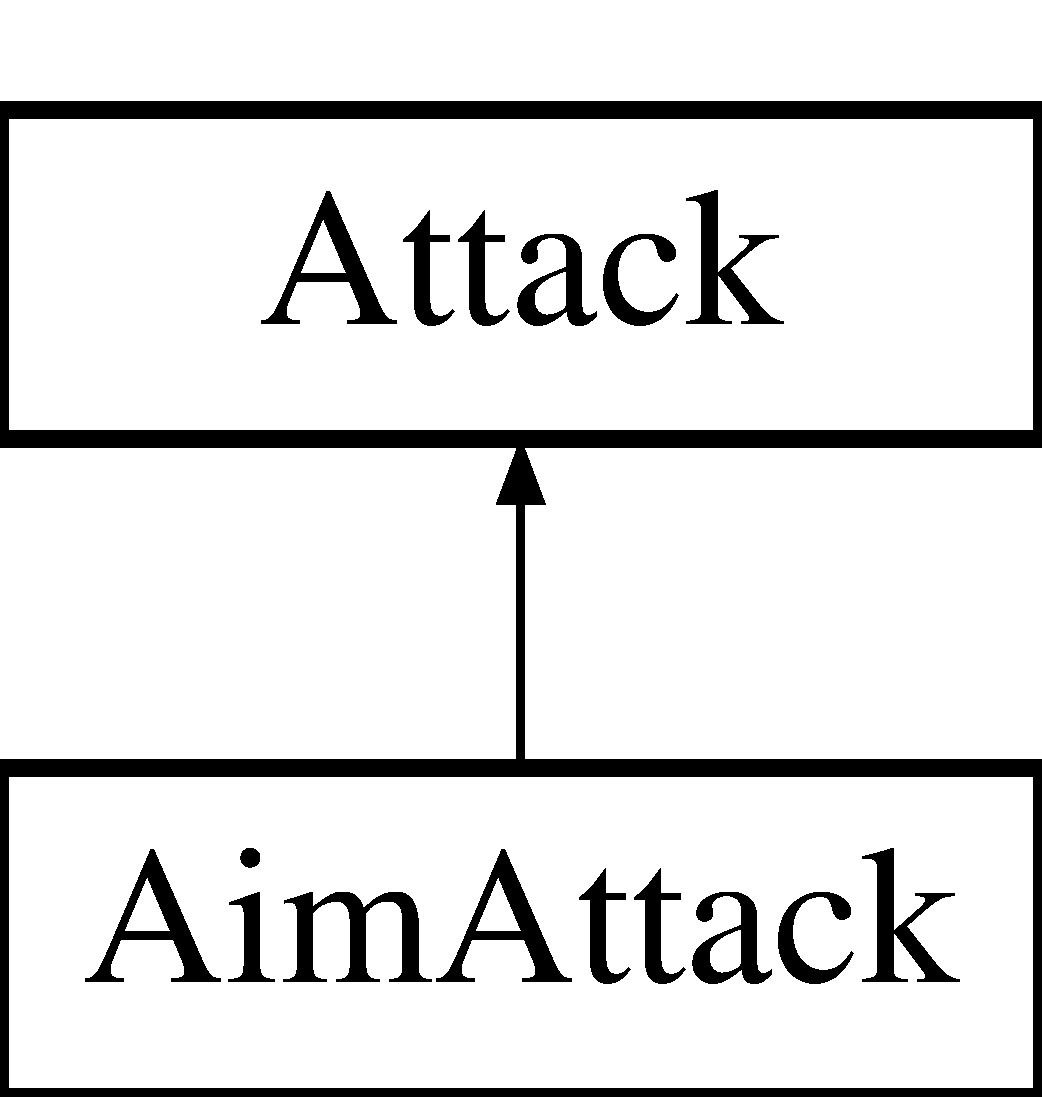
\includegraphics[height=2.000000cm]{class_aim_attack}
\end{center}
\end{figure}
\subsection*{公開メンバ関数}
\begin{DoxyCompactItemize}
\item 
\hyperlink{class_aim_attack_aa83ba425f1fb3e75df716419fb724710}{Aim\+Attack} (int damage, int speed, int interval, \hyperlink{class_character}{Character} $\ast$chara)
\item 
void \hyperlink{class_aim_attack_a965a7108493329d5d4b869e7289a3835}{Initialize\+Bullet} (int num)
\item 
void \hyperlink{class_aim_attack_abc5f35b870b83aecd372e5b3aef30b37}{Do\+Attack} ()
\end{DoxyCompactItemize}
\subsection*{その他の継承メンバ}


\subsection{構築子と解体子}
\hypertarget{class_aim_attack_aa83ba425f1fb3e75df716419fb724710}{\index{Aim\+Attack@{Aim\+Attack}!Aim\+Attack@{Aim\+Attack}}
\index{Aim\+Attack@{Aim\+Attack}!Aim\+Attack@{Aim\+Attack}}
\subsubsection[{Aim\+Attack}]{\setlength{\rightskip}{0pt plus 5cm}Aim\+Attack\+::\+Aim\+Attack (
\begin{DoxyParamCaption}
\item[{int}]{damage, }
\item[{int}]{speed, }
\item[{int}]{interval, }
\item[{{\bf Character} $\ast$}]{chara}
\end{DoxyParamCaption}
)}}\label{class_aim_attack_aa83ba425f1fb3e75df716419fb724710}


\subsection{関数詳解}
\hypertarget{class_aim_attack_abc5f35b870b83aecd372e5b3aef30b37}{\index{Aim\+Attack@{Aim\+Attack}!Do\+Attack@{Do\+Attack}}
\index{Do\+Attack@{Do\+Attack}!Aim\+Attack@{Aim\+Attack}}
\subsubsection[{Do\+Attack}]{\setlength{\rightskip}{0pt plus 5cm}void Aim\+Attack\+::\+Do\+Attack (
\begin{DoxyParamCaption}
{}
\end{DoxyParamCaption}
)\hspace{0.3cm}{\ttfamily [virtual]}}}\label{class_aim_attack_abc5f35b870b83aecd372e5b3aef30b37}


\hyperlink{class_attack_a06d145ff7c11cfef2b688eefcd11dac1}{Attack}を実装しています。

\hypertarget{class_aim_attack_a965a7108493329d5d4b869e7289a3835}{\index{Aim\+Attack@{Aim\+Attack}!Initialize\+Bullet@{Initialize\+Bullet}}
\index{Initialize\+Bullet@{Initialize\+Bullet}!Aim\+Attack@{Aim\+Attack}}
\subsubsection[{Initialize\+Bullet}]{\setlength{\rightskip}{0pt plus 5cm}void Aim\+Attack\+::\+Initialize\+Bullet (
\begin{DoxyParamCaption}
\item[{int}]{num}
\end{DoxyParamCaption}
)\hspace{0.3cm}{\ttfamily [virtual]}}}\label{class_aim_attack_a965a7108493329d5d4b869e7289a3835}


\hyperlink{class_attack_ac02b84493ca19adf8425c1ed2efaf54c}{Attack}を実装しています。



このクラス詳解は次のファイルから抽出されました\+:\begin{DoxyCompactItemize}
\item 
\hyperlink{_aim_attack_8h}{Aim\+Attack.\+h}\item 
\hyperlink{_aim_attack_8cpp}{Aim\+Attack.\+cpp}\end{DoxyCompactItemize}

\hypertarget{class_aim_bullet}{\section{Aim\+Bullet クラス}
\label{class_aim_bullet}\index{Aim\+Bullet@{Aim\+Bullet}}
}


{\ttfamily \#include $<$Aim\+Bullet.\+h$>$}

Aim\+Bullet の継承関係図\begin{figure}[H]
\begin{center}
\leavevmode
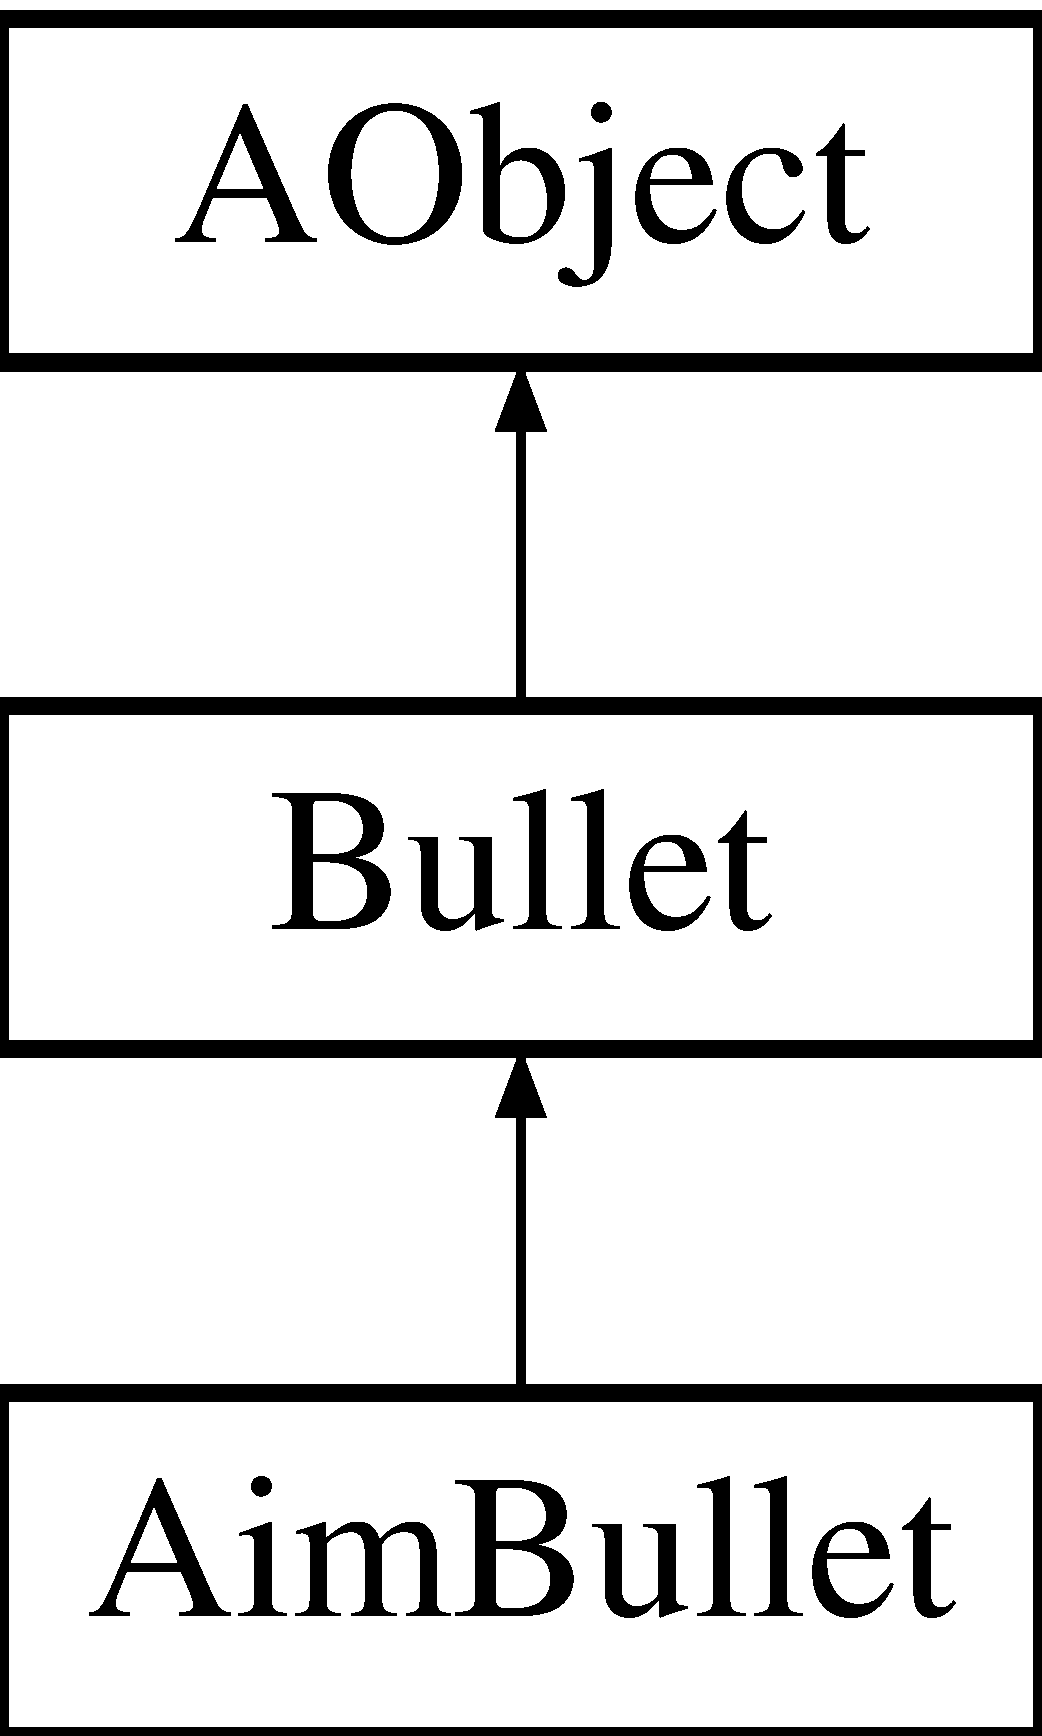
\includegraphics[height=3.000000cm]{class_aim_bullet}
\end{center}
\end{figure}
\subsection*{公開メンバ関数}
\begin{DoxyCompactItemize}
\item 
\hyperlink{class_aim_bullet_a17f0f2518c17e14a45a3db64640830ac}{Aim\+Bullet} (double x, double y, int \hyperlink{class_bullet_a6e5b78574ec8fbff411b1319cf111799}{damage}, int \hyperlink{class_a_object_abb924b7e558a2f9d86f2db2bc2fb18a4}{speed}, double hit\+\_\+size\+\_\+x, double hit\+\_\+size\+\_\+y, double aim\+\_\+x, double aim\+\_\+y)
\item 
void \hyperlink{class_aim_bullet_aaf567ed7c1e05f982c443de279b27d13}{Initialize} (double x, double y, double aim\+\_\+x, double aim\+\_\+y)
\item 
\hyperlink{class_aim_bullet_a037ba3088af67ddfd5ede933fd7f68e4}{$\sim$\+Aim\+Bullet} (void)
\end{DoxyCompactItemize}
\subsection*{その他の継承メンバ}


\subsection{構築子と解体子}
\hypertarget{class_aim_bullet_a17f0f2518c17e14a45a3db64640830ac}{\index{Aim\+Bullet@{Aim\+Bullet}!Aim\+Bullet@{Aim\+Bullet}}
\index{Aim\+Bullet@{Aim\+Bullet}!Aim\+Bullet@{Aim\+Bullet}}
\subsubsection[{Aim\+Bullet}]{\setlength{\rightskip}{0pt plus 5cm}Aim\+Bullet\+::\+Aim\+Bullet (
\begin{DoxyParamCaption}
\item[{double}]{x, }
\item[{double}]{y, }
\item[{int}]{damage, }
\item[{int}]{speed, }
\item[{double}]{hit\+\_\+size\+\_\+x, }
\item[{double}]{hit\+\_\+size\+\_\+y, }
\item[{double}]{aim\+\_\+x, }
\item[{double}]{aim\+\_\+y}
\end{DoxyParamCaption}
)}}\label{class_aim_bullet_a17f0f2518c17e14a45a3db64640830ac}
\hypertarget{class_aim_bullet_a037ba3088af67ddfd5ede933fd7f68e4}{\index{Aim\+Bullet@{Aim\+Bullet}!````~Aim\+Bullet@{$\sim$\+Aim\+Bullet}}
\index{````~Aim\+Bullet@{$\sim$\+Aim\+Bullet}!Aim\+Bullet@{Aim\+Bullet}}
\subsubsection[{$\sim$\+Aim\+Bullet}]{\setlength{\rightskip}{0pt plus 5cm}Aim\+Bullet\+::$\sim$\+Aim\+Bullet (
\begin{DoxyParamCaption}
\item[{void}]{}
\end{DoxyParamCaption}
)}}\label{class_aim_bullet_a037ba3088af67ddfd5ede933fd7f68e4}


\subsection{関数詳解}
\hypertarget{class_aim_bullet_aaf567ed7c1e05f982c443de279b27d13}{\index{Aim\+Bullet@{Aim\+Bullet}!Initialize@{Initialize}}
\index{Initialize@{Initialize}!Aim\+Bullet@{Aim\+Bullet}}
\subsubsection[{Initialize}]{\setlength{\rightskip}{0pt plus 5cm}void Aim\+Bullet\+::\+Initialize (
\begin{DoxyParamCaption}
\item[{double}]{x, }
\item[{double}]{y, }
\item[{double}]{aim\+\_\+x, }
\item[{double}]{aim\+\_\+y}
\end{DoxyParamCaption}
)}}\label{class_aim_bullet_aaf567ed7c1e05f982c443de279b27d13}


このクラス詳解は次のファイルから抽出されました\+:\begin{DoxyCompactItemize}
\item 
\hyperlink{_aim_bullet_8h}{Aim\+Bullet.\+h}\item 
\hyperlink{_aim_bullet_8cpp}{Aim\+Bullet.\+cpp}\end{DoxyCompactItemize}

\hypertarget{class_a_object}{\section{A\+Object クラス}
\label{class_a_object}\index{A\+Object@{A\+Object}}
}


{\ttfamily \#include $<$A\+Object.\+h$>$}

A\+Object の継承関係図\begin{figure}[H]
\begin{center}
\leavevmode
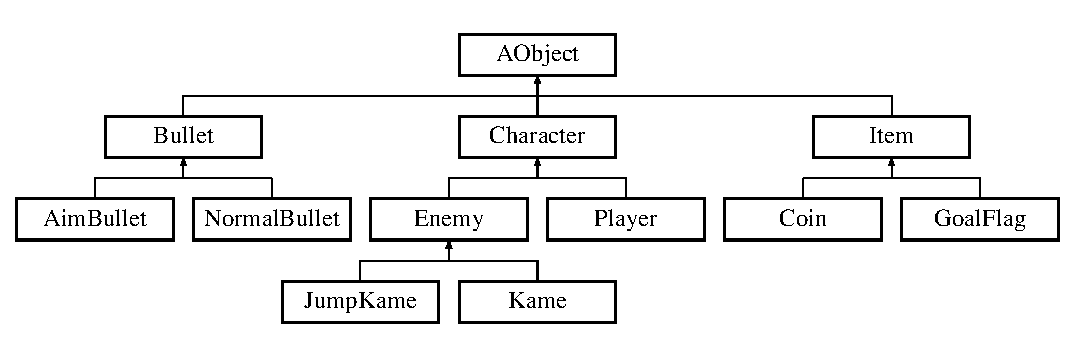
\includegraphics[height=4.000000cm]{class_a_object}
\end{center}
\end{figure}
\subsection*{公開メンバ関数}
\begin{DoxyCompactItemize}
\item 
\hyperlink{class_a_object_a1956c3120bdc7f0372a5aab8c0b1cbb6}{A\+Object} (double ax, double ay, char $\ast$fname, int hit\+\_\+size\+\_\+x, int hit\+\_\+size\+\_\+y, bool \hyperlink{class_a_object_a7453abe76bbddf446aa5787231428a52}{right})
\item 
virtual void \hyperlink{class_a_object_aa07f4874e508e22cc0980e5ab6eb7f54}{Reset} ()
\item 
void \hyperlink{class_a_object_a60fae4021ac710983beefcf8cdb7f3bd}{Move} ()
\item 
virtual void \hyperlink{class_a_object_a0e279a93c79be5807e9bbd20875369a2}{Draw} (int offset)
\item 
virtual void \hyperlink{class_a_object_a61f89197cb14b1270a0a232ee88333a0}{Think} ()=0
\item 
void \hyperlink{class_a_object_a95c42b1bcef8f364389d9cf131a37921}{Fall} (double gravity)
\item 
void \hyperlink{class_a_object_a6661473a035f6e0ee0e7d98182630389}{Die} ()
\item 
void \hyperlink{class_a_object_aab646016a7b8d3040e2e3675e74d0629}{Revival} ()
\item 
void \hyperlink{class_a_object_a5266e7cb202fc1c27ac66fb8372410cb}{Set\+\_\+\+Speed} (double speed\+\_\+x, double speed\+\_\+y)
\item 
void \hyperlink{class_a_object_a6547fb1f7e3b5c5aab84b0b787e2869c}{Touched\+Block\+X} (double set\+\_\+x)
\item 
void \hyperlink{class_a_object_acfe5d595ef8c3387b1bbba51cb397602}{Touched\+Block\+Y} (double set\+\_\+y)
\item 
void \hyperlink{class_a_object_aa4d5ec1e9ece904effd747657f4e4530}{Get\+Object\+Size} ()
\item 
double \hyperlink{class_a_object_af18a89079a95159f7b93a92a921f4b54}{Get\+Center\+Pos\+X} ()
\item 
double \hyperlink{class_a_object_a33c32784ef245183b0207811c0f88521}{Get\+Center\+Pos\+Y} ()
\item 
\hyperlink{struct_two_dimension}{Two\+Dimension} \hyperlink{class_a_object_a71a4ba584e2a76b73ed623deeb7d1358}{pos} ()
\item 
\hyperlink{struct_two_dimension}{Two\+Dimension} \hyperlink{class_a_object_abb924b7e558a2f9d86f2db2bc2fb18a4}{speed} ()
\item 
\hyperlink{struct_two_dimension}{Two\+Dimension} \hyperlink{class_a_object_a42d73d2bad560ba5d83a1b7193347c48}{size} ()
\item 
\hyperlink{struct_two_dimension}{Two\+Dimension} \hyperlink{class_a_object_a3505a72b54c24e488b7daa64161f9ca6}{hit\+\_\+size} ()
\item 
bool \hyperlink{class_a_object_a2ceff5dd8626fcc399e583ce2b204200}{is\+Aerial} ()
\item 
bool \hyperlink{class_a_object_aa02494588289ed9662abd082bdec716d}{is\+Right} ()
\item 
bool \hyperlink{class_a_object_ac26a24066236bc7d4f8cc4324a4ae01f}{is\+Alive} ()
\item 
int \hyperlink{class_a_object_a0bfe4dc75e67969c28cda83f301e84ec}{object\+\_\+type} ()
\end{DoxyCompactItemize}
\subsection*{限定公開変数類}
\begin{DoxyCompactItemize}
\item 
int \hyperlink{class_a_object_abf9e02eedf75207898d7059bb6815819}{live\+\_\+count\+\_\+}
\item 
int \hyperlink{class_a_object_a1f9d082036ee3272dacb9a732fa7cdcc}{graphic\+\_\+handle\+\_\+}
\item 
int \hyperlink{class_a_object_a00038f72ce7400697c2be7f4fdd15d77}{move\+\_\+ghandle\+\_\+}
\item 
\hyperlink{struct_two_dimension}{Two\+Dimension} \hyperlink{class_a_object_aff37fc81435924247fe0e4d7fa0186cf}{pos\+\_\+}
\item 
\hyperlink{struct_two_dimension}{Two\+Dimension} \hyperlink{class_a_object_a7d817eebc8b7151ff99d48c16c94b73f}{first\+\_\+pos\+\_\+}
\item 
\hyperlink{struct_two_dimension}{Two\+Dimension} \hyperlink{class_a_object_a640b3a323c205046b20640123222cdd3}{speed\+\_\+}
\item 
\hyperlink{struct_two_dimension}{Two\+Dimension} \hyperlink{class_a_object_a50bc88cfccd518e158096b5f033c0728}{size\+\_\+}
\item 
\hyperlink{struct_two_dimension}{Two\+Dimension} \hyperlink{class_a_object_a893dc760682c3fbafc5c96229939a8ec}{hit\+\_\+size\+\_\+}
\item 
bool \hyperlink{class_a_object_a98663f6d7145a2b7fc2009f95804325a}{alive}
\item 
bool \hyperlink{class_a_object_a7453abe76bbddf446aa5787231428a52}{right}
\item 
bool \hyperlink{class_a_object_aad0f6917ebc7fb2e44163302a67638a6}{first\+\_\+right}
\item 
bool \hyperlink{class_a_object_a0396b51efa313b95783f3582f1327ad1}{aerial}
\item 
int \hyperlink{class_a_object_a47a6ff0cef7449975ce63f07aade9d5d}{object\+\_\+type\+\_\+}
\end{DoxyCompactItemize}
\subsection*{静的限定公開変数類}
\begin{DoxyCompactItemize}
\item 
static \hyperlink{class_load_graphic}{Load\+Graphic} \hyperlink{class_a_object_a18177a7a13f626091e935c1846b7607a}{loadg} =\hyperlink{class_load_graphic}{Load\+Graphic}()
\end{DoxyCompactItemize}


\subsection{構築子と解体子}
\hypertarget{class_a_object_a1956c3120bdc7f0372a5aab8c0b1cbb6}{\index{A\+Object@{A\+Object}!A\+Object@{A\+Object}}
\index{A\+Object@{A\+Object}!A\+Object@{A\+Object}}
\subsubsection[{A\+Object}]{\setlength{\rightskip}{0pt plus 5cm}A\+Object\+::\+A\+Object (
\begin{DoxyParamCaption}
\item[{double}]{ax, }
\item[{double}]{ay, }
\item[{char $\ast$}]{fname, }
\item[{int}]{hit\+\_\+size\+\_\+x, }
\item[{int}]{hit\+\_\+size\+\_\+y, }
\item[{bool}]{right}
\end{DoxyParamCaption}
)}}\label{class_a_object_a1956c3120bdc7f0372a5aab8c0b1cbb6}


\subsection{関数詳解}
\hypertarget{class_a_object_a6661473a035f6e0ee0e7d98182630389}{\index{A\+Object@{A\+Object}!Die@{Die}}
\index{Die@{Die}!A\+Object@{A\+Object}}
\subsubsection[{Die}]{\setlength{\rightskip}{0pt plus 5cm}void A\+Object\+::\+Die (
\begin{DoxyParamCaption}
{}
\end{DoxyParamCaption}
)}}\label{class_a_object_a6661473a035f6e0ee0e7d98182630389}
\hypertarget{class_a_object_a0e279a93c79be5807e9bbd20875369a2}{\index{A\+Object@{A\+Object}!Draw@{Draw}}
\index{Draw@{Draw}!A\+Object@{A\+Object}}
\subsubsection[{Draw}]{\setlength{\rightskip}{0pt plus 5cm}void A\+Object\+::\+Draw (
\begin{DoxyParamCaption}
\item[{int}]{offset}
\end{DoxyParamCaption}
)\hspace{0.3cm}{\ttfamily [virtual]}}}\label{class_a_object_a0e279a93c79be5807e9bbd20875369a2}


\hyperlink{class_character_ad359a991510783008ee96060f247c990}{Character}, \hyperlink{class_player_a5e32dec9258cfa8145e482fed4c42c83}{Player}で再実装されています。

\hypertarget{class_a_object_a95c42b1bcef8f364389d9cf131a37921}{\index{A\+Object@{A\+Object}!Fall@{Fall}}
\index{Fall@{Fall}!A\+Object@{A\+Object}}
\subsubsection[{Fall}]{\setlength{\rightskip}{0pt plus 5cm}void A\+Object\+::\+Fall (
\begin{DoxyParamCaption}
\item[{double}]{gravity}
\end{DoxyParamCaption}
)}}\label{class_a_object_a95c42b1bcef8f364389d9cf131a37921}
\hypertarget{class_a_object_af18a89079a95159f7b93a92a921f4b54}{\index{A\+Object@{A\+Object}!Get\+Center\+Pos\+X@{Get\+Center\+Pos\+X}}
\index{Get\+Center\+Pos\+X@{Get\+Center\+Pos\+X}!A\+Object@{A\+Object}}
\subsubsection[{Get\+Center\+Pos\+X}]{\setlength{\rightskip}{0pt plus 5cm}double A\+Object\+::\+Get\+Center\+Pos\+X (
\begin{DoxyParamCaption}
{}
\end{DoxyParamCaption}
)}}\label{class_a_object_af18a89079a95159f7b93a92a921f4b54}
\hypertarget{class_a_object_a33c32784ef245183b0207811c0f88521}{\index{A\+Object@{A\+Object}!Get\+Center\+Pos\+Y@{Get\+Center\+Pos\+Y}}
\index{Get\+Center\+Pos\+Y@{Get\+Center\+Pos\+Y}!A\+Object@{A\+Object}}
\subsubsection[{Get\+Center\+Pos\+Y}]{\setlength{\rightskip}{0pt plus 5cm}double A\+Object\+::\+Get\+Center\+Pos\+Y (
\begin{DoxyParamCaption}
{}
\end{DoxyParamCaption}
)}}\label{class_a_object_a33c32784ef245183b0207811c0f88521}
\hypertarget{class_a_object_aa4d5ec1e9ece904effd747657f4e4530}{\index{A\+Object@{A\+Object}!Get\+Object\+Size@{Get\+Object\+Size}}
\index{Get\+Object\+Size@{Get\+Object\+Size}!A\+Object@{A\+Object}}
\subsubsection[{Get\+Object\+Size}]{\setlength{\rightskip}{0pt plus 5cm}void A\+Object\+::\+Get\+Object\+Size (
\begin{DoxyParamCaption}
{}
\end{DoxyParamCaption}
)}}\label{class_a_object_aa4d5ec1e9ece904effd747657f4e4530}
\hypertarget{class_a_object_a3505a72b54c24e488b7daa64161f9ca6}{\index{A\+Object@{A\+Object}!hit\+\_\+size@{hit\+\_\+size}}
\index{hit\+\_\+size@{hit\+\_\+size}!A\+Object@{A\+Object}}
\subsubsection[{hit\+\_\+size}]{\setlength{\rightskip}{0pt plus 5cm}{\bf Two\+Dimension} A\+Object\+::hit\+\_\+size (
\begin{DoxyParamCaption}
{}
\end{DoxyParamCaption}
)\hspace{0.3cm}{\ttfamily [inline]}}}\label{class_a_object_a3505a72b54c24e488b7daa64161f9ca6}
\hypertarget{class_a_object_a2ceff5dd8626fcc399e583ce2b204200}{\index{A\+Object@{A\+Object}!is\+Aerial@{is\+Aerial}}
\index{is\+Aerial@{is\+Aerial}!A\+Object@{A\+Object}}
\subsubsection[{is\+Aerial}]{\setlength{\rightskip}{0pt plus 5cm}bool A\+Object\+::is\+Aerial (
\begin{DoxyParamCaption}
{}
\end{DoxyParamCaption}
)\hspace{0.3cm}{\ttfamily [inline]}}}\label{class_a_object_a2ceff5dd8626fcc399e583ce2b204200}
\hypertarget{class_a_object_ac26a24066236bc7d4f8cc4324a4ae01f}{\index{A\+Object@{A\+Object}!is\+Alive@{is\+Alive}}
\index{is\+Alive@{is\+Alive}!A\+Object@{A\+Object}}
\subsubsection[{is\+Alive}]{\setlength{\rightskip}{0pt plus 5cm}bool A\+Object\+::is\+Alive (
\begin{DoxyParamCaption}
{}
\end{DoxyParamCaption}
)\hspace{0.3cm}{\ttfamily [inline]}}}\label{class_a_object_ac26a24066236bc7d4f8cc4324a4ae01f}
\hypertarget{class_a_object_aa02494588289ed9662abd082bdec716d}{\index{A\+Object@{A\+Object}!is\+Right@{is\+Right}}
\index{is\+Right@{is\+Right}!A\+Object@{A\+Object}}
\subsubsection[{is\+Right}]{\setlength{\rightskip}{0pt plus 5cm}bool A\+Object\+::is\+Right (
\begin{DoxyParamCaption}
{}
\end{DoxyParamCaption}
)\hspace{0.3cm}{\ttfamily [inline]}}}\label{class_a_object_aa02494588289ed9662abd082bdec716d}
\hypertarget{class_a_object_a60fae4021ac710983beefcf8cdb7f3bd}{\index{A\+Object@{A\+Object}!Move@{Move}}
\index{Move@{Move}!A\+Object@{A\+Object}}
\subsubsection[{Move}]{\setlength{\rightskip}{0pt plus 5cm}void A\+Object\+::\+Move (
\begin{DoxyParamCaption}
{}
\end{DoxyParamCaption}
)}}\label{class_a_object_a60fae4021ac710983beefcf8cdb7f3bd}
\hypertarget{class_a_object_a0bfe4dc75e67969c28cda83f301e84ec}{\index{A\+Object@{A\+Object}!object\+\_\+type@{object\+\_\+type}}
\index{object\+\_\+type@{object\+\_\+type}!A\+Object@{A\+Object}}
\subsubsection[{object\+\_\+type}]{\setlength{\rightskip}{0pt plus 5cm}int A\+Object\+::object\+\_\+type (
\begin{DoxyParamCaption}
{}
\end{DoxyParamCaption}
)\hspace{0.3cm}{\ttfamily [inline]}}}\label{class_a_object_a0bfe4dc75e67969c28cda83f301e84ec}
\hypertarget{class_a_object_a71a4ba584e2a76b73ed623deeb7d1358}{\index{A\+Object@{A\+Object}!pos@{pos}}
\index{pos@{pos}!A\+Object@{A\+Object}}
\subsubsection[{pos}]{\setlength{\rightskip}{0pt plus 5cm}{\bf Two\+Dimension} A\+Object\+::pos (
\begin{DoxyParamCaption}
{}
\end{DoxyParamCaption}
)\hspace{0.3cm}{\ttfamily [inline]}}}\label{class_a_object_a71a4ba584e2a76b73ed623deeb7d1358}
\hypertarget{class_a_object_aa07f4874e508e22cc0980e5ab6eb7f54}{\index{A\+Object@{A\+Object}!Reset@{Reset}}
\index{Reset@{Reset}!A\+Object@{A\+Object}}
\subsubsection[{Reset}]{\setlength{\rightskip}{0pt plus 5cm}void A\+Object\+::\+Reset (
\begin{DoxyParamCaption}
{}
\end{DoxyParamCaption}
)\hspace{0.3cm}{\ttfamily [virtual]}}}\label{class_a_object_aa07f4874e508e22cc0980e5ab6eb7f54}


\hyperlink{class_character_a6c1fa20d22b5ea6edc4dbd6ca9496411}{Character}, \hyperlink{class_player_a22a0d2b901622c497b677b7c75fafe45}{Player}で再実装されています。

\hypertarget{class_a_object_aab646016a7b8d3040e2e3675e74d0629}{\index{A\+Object@{A\+Object}!Revival@{Revival}}
\index{Revival@{Revival}!A\+Object@{A\+Object}}
\subsubsection[{Revival}]{\setlength{\rightskip}{0pt plus 5cm}void A\+Object\+::\+Revival (
\begin{DoxyParamCaption}
{}
\end{DoxyParamCaption}
)\hspace{0.3cm}{\ttfamily [inline]}}}\label{class_a_object_aab646016a7b8d3040e2e3675e74d0629}
\hypertarget{class_a_object_a5266e7cb202fc1c27ac66fb8372410cb}{\index{A\+Object@{A\+Object}!Set\+\_\+\+Speed@{Set\+\_\+\+Speed}}
\index{Set\+\_\+\+Speed@{Set\+\_\+\+Speed}!A\+Object@{A\+Object}}
\subsubsection[{Set\+\_\+\+Speed}]{\setlength{\rightskip}{0pt plus 5cm}void A\+Object\+::\+Set\+\_\+\+Speed (
\begin{DoxyParamCaption}
\item[{double}]{speed\+\_\+x, }
\item[{double}]{speed\+\_\+y}
\end{DoxyParamCaption}
)}}\label{class_a_object_a5266e7cb202fc1c27ac66fb8372410cb}
\hypertarget{class_a_object_a42d73d2bad560ba5d83a1b7193347c48}{\index{A\+Object@{A\+Object}!size@{size}}
\index{size@{size}!A\+Object@{A\+Object}}
\subsubsection[{size}]{\setlength{\rightskip}{0pt plus 5cm}{\bf Two\+Dimension} A\+Object\+::size (
\begin{DoxyParamCaption}
{}
\end{DoxyParamCaption}
)\hspace{0.3cm}{\ttfamily [inline]}}}\label{class_a_object_a42d73d2bad560ba5d83a1b7193347c48}
\hypertarget{class_a_object_abb924b7e558a2f9d86f2db2bc2fb18a4}{\index{A\+Object@{A\+Object}!speed@{speed}}
\index{speed@{speed}!A\+Object@{A\+Object}}
\subsubsection[{speed}]{\setlength{\rightskip}{0pt plus 5cm}{\bf Two\+Dimension} A\+Object\+::speed (
\begin{DoxyParamCaption}
{}
\end{DoxyParamCaption}
)\hspace{0.3cm}{\ttfamily [inline]}}}\label{class_a_object_abb924b7e558a2f9d86f2db2bc2fb18a4}
\hypertarget{class_a_object_a61f89197cb14b1270a0a232ee88333a0}{\index{A\+Object@{A\+Object}!Think@{Think}}
\index{Think@{Think}!A\+Object@{A\+Object}}
\subsubsection[{Think}]{\setlength{\rightskip}{0pt plus 5cm}void A\+Object\+::\+Think (
\begin{DoxyParamCaption}
{}
\end{DoxyParamCaption}
)\hspace{0.3cm}{\ttfamily [pure virtual]}}}\label{class_a_object_a61f89197cb14b1270a0a232ee88333a0}


\hyperlink{class_character_a953e7c76dce887426f74e568e5ebbe39}{Character}, \hyperlink{class_coin_a3bfc309bcea6da0bda2913ffc20adbdd}{Coin}, \hyperlink{class_bullet_a0f3207f4dc7244fd3510b89943f939f3}{Bullet}, \hyperlink{class_goal_flag_a343f277b68067d9d19bff4815b14c6ac}{Goal\+Flag}で実装されています。

\hypertarget{class_a_object_a6547fb1f7e3b5c5aab84b0b787e2869c}{\index{A\+Object@{A\+Object}!Touched\+Block\+X@{Touched\+Block\+X}}
\index{Touched\+Block\+X@{Touched\+Block\+X}!A\+Object@{A\+Object}}
\subsubsection[{Touched\+Block\+X}]{\setlength{\rightskip}{0pt plus 5cm}void A\+Object\+::\+Touched\+Block\+X (
\begin{DoxyParamCaption}
\item[{double}]{set\+\_\+x}
\end{DoxyParamCaption}
)}}\label{class_a_object_a6547fb1f7e3b5c5aab84b0b787e2869c}
\hypertarget{class_a_object_acfe5d595ef8c3387b1bbba51cb397602}{\index{A\+Object@{A\+Object}!Touched\+Block\+Y@{Touched\+Block\+Y}}
\index{Touched\+Block\+Y@{Touched\+Block\+Y}!A\+Object@{A\+Object}}
\subsubsection[{Touched\+Block\+Y}]{\setlength{\rightskip}{0pt plus 5cm}void A\+Object\+::\+Touched\+Block\+Y (
\begin{DoxyParamCaption}
\item[{double}]{set\+\_\+y}
\end{DoxyParamCaption}
)}}\label{class_a_object_acfe5d595ef8c3387b1bbba51cb397602}


\subsection{メンバ詳解}
\hypertarget{class_a_object_a0396b51efa313b95783f3582f1327ad1}{\index{A\+Object@{A\+Object}!aerial@{aerial}}
\index{aerial@{aerial}!A\+Object@{A\+Object}}
\subsubsection[{aerial}]{\setlength{\rightskip}{0pt plus 5cm}bool A\+Object\+::aerial\hspace{0.3cm}{\ttfamily [protected]}}}\label{class_a_object_a0396b51efa313b95783f3582f1327ad1}
\hypertarget{class_a_object_a98663f6d7145a2b7fc2009f95804325a}{\index{A\+Object@{A\+Object}!alive@{alive}}
\index{alive@{alive}!A\+Object@{A\+Object}}
\subsubsection[{alive}]{\setlength{\rightskip}{0pt plus 5cm}bool A\+Object\+::alive\hspace{0.3cm}{\ttfamily [protected]}}}\label{class_a_object_a98663f6d7145a2b7fc2009f95804325a}
\hypertarget{class_a_object_a7d817eebc8b7151ff99d48c16c94b73f}{\index{A\+Object@{A\+Object}!first\+\_\+pos\+\_\+@{first\+\_\+pos\+\_\+}}
\index{first\+\_\+pos\+\_\+@{first\+\_\+pos\+\_\+}!A\+Object@{A\+Object}}
\subsubsection[{first\+\_\+pos\+\_\+}]{\setlength{\rightskip}{0pt plus 5cm}{\bf Two\+Dimension} A\+Object\+::first\+\_\+pos\+\_\+\hspace{0.3cm}{\ttfamily [protected]}}}\label{class_a_object_a7d817eebc8b7151ff99d48c16c94b73f}
\hypertarget{class_a_object_aad0f6917ebc7fb2e44163302a67638a6}{\index{A\+Object@{A\+Object}!first\+\_\+right@{first\+\_\+right}}
\index{first\+\_\+right@{first\+\_\+right}!A\+Object@{A\+Object}}
\subsubsection[{first\+\_\+right}]{\setlength{\rightskip}{0pt plus 5cm}bool A\+Object\+::first\+\_\+right\hspace{0.3cm}{\ttfamily [protected]}}}\label{class_a_object_aad0f6917ebc7fb2e44163302a67638a6}
\hypertarget{class_a_object_a1f9d082036ee3272dacb9a732fa7cdcc}{\index{A\+Object@{A\+Object}!graphic\+\_\+handle\+\_\+@{graphic\+\_\+handle\+\_\+}}
\index{graphic\+\_\+handle\+\_\+@{graphic\+\_\+handle\+\_\+}!A\+Object@{A\+Object}}
\subsubsection[{graphic\+\_\+handle\+\_\+}]{\setlength{\rightskip}{0pt plus 5cm}int A\+Object\+::graphic\+\_\+handle\+\_\+\hspace{0.3cm}{\ttfamily [protected]}}}\label{class_a_object_a1f9d082036ee3272dacb9a732fa7cdcc}
\hypertarget{class_a_object_a893dc760682c3fbafc5c96229939a8ec}{\index{A\+Object@{A\+Object}!hit\+\_\+size\+\_\+@{hit\+\_\+size\+\_\+}}
\index{hit\+\_\+size\+\_\+@{hit\+\_\+size\+\_\+}!A\+Object@{A\+Object}}
\subsubsection[{hit\+\_\+size\+\_\+}]{\setlength{\rightskip}{0pt plus 5cm}{\bf Two\+Dimension} A\+Object\+::hit\+\_\+size\+\_\+\hspace{0.3cm}{\ttfamily [protected]}}}\label{class_a_object_a893dc760682c3fbafc5c96229939a8ec}
\hypertarget{class_a_object_abf9e02eedf75207898d7059bb6815819}{\index{A\+Object@{A\+Object}!live\+\_\+count\+\_\+@{live\+\_\+count\+\_\+}}
\index{live\+\_\+count\+\_\+@{live\+\_\+count\+\_\+}!A\+Object@{A\+Object}}
\subsubsection[{live\+\_\+count\+\_\+}]{\setlength{\rightskip}{0pt plus 5cm}int A\+Object\+::live\+\_\+count\+\_\+\hspace{0.3cm}{\ttfamily [protected]}}}\label{class_a_object_abf9e02eedf75207898d7059bb6815819}
\hypertarget{class_a_object_a18177a7a13f626091e935c1846b7607a}{\index{A\+Object@{A\+Object}!loadg@{loadg}}
\index{loadg@{loadg}!A\+Object@{A\+Object}}
\subsubsection[{loadg}]{\setlength{\rightskip}{0pt plus 5cm}{\bf Load\+Graphic} A\+Object\+::loadg ={\bf Load\+Graphic}()\hspace{0.3cm}{\ttfamily [static]}, {\ttfamily [protected]}}}\label{class_a_object_a18177a7a13f626091e935c1846b7607a}
\hypertarget{class_a_object_a00038f72ce7400697c2be7f4fdd15d77}{\index{A\+Object@{A\+Object}!move\+\_\+ghandle\+\_\+@{move\+\_\+ghandle\+\_\+}}
\index{move\+\_\+ghandle\+\_\+@{move\+\_\+ghandle\+\_\+}!A\+Object@{A\+Object}}
\subsubsection[{move\+\_\+ghandle\+\_\+}]{\setlength{\rightskip}{0pt plus 5cm}int A\+Object\+::move\+\_\+ghandle\+\_\+\hspace{0.3cm}{\ttfamily [protected]}}}\label{class_a_object_a00038f72ce7400697c2be7f4fdd15d77}
\hypertarget{class_a_object_a47a6ff0cef7449975ce63f07aade9d5d}{\index{A\+Object@{A\+Object}!object\+\_\+type\+\_\+@{object\+\_\+type\+\_\+}}
\index{object\+\_\+type\+\_\+@{object\+\_\+type\+\_\+}!A\+Object@{A\+Object}}
\subsubsection[{object\+\_\+type\+\_\+}]{\setlength{\rightskip}{0pt plus 5cm}int A\+Object\+::object\+\_\+type\+\_\+\hspace{0.3cm}{\ttfamily [protected]}}}\label{class_a_object_a47a6ff0cef7449975ce63f07aade9d5d}
\hypertarget{class_a_object_aff37fc81435924247fe0e4d7fa0186cf}{\index{A\+Object@{A\+Object}!pos\+\_\+@{pos\+\_\+}}
\index{pos\+\_\+@{pos\+\_\+}!A\+Object@{A\+Object}}
\subsubsection[{pos\+\_\+}]{\setlength{\rightskip}{0pt plus 5cm}{\bf Two\+Dimension} A\+Object\+::pos\+\_\+\hspace{0.3cm}{\ttfamily [protected]}}}\label{class_a_object_aff37fc81435924247fe0e4d7fa0186cf}
\hypertarget{class_a_object_a7453abe76bbddf446aa5787231428a52}{\index{A\+Object@{A\+Object}!right@{right}}
\index{right@{right}!A\+Object@{A\+Object}}
\subsubsection[{right}]{\setlength{\rightskip}{0pt plus 5cm}bool A\+Object\+::right\hspace{0.3cm}{\ttfamily [protected]}}}\label{class_a_object_a7453abe76bbddf446aa5787231428a52}
\hypertarget{class_a_object_a50bc88cfccd518e158096b5f033c0728}{\index{A\+Object@{A\+Object}!size\+\_\+@{size\+\_\+}}
\index{size\+\_\+@{size\+\_\+}!A\+Object@{A\+Object}}
\subsubsection[{size\+\_\+}]{\setlength{\rightskip}{0pt plus 5cm}{\bf Two\+Dimension} A\+Object\+::size\+\_\+\hspace{0.3cm}{\ttfamily [protected]}}}\label{class_a_object_a50bc88cfccd518e158096b5f033c0728}
\hypertarget{class_a_object_a640b3a323c205046b20640123222cdd3}{\index{A\+Object@{A\+Object}!speed\+\_\+@{speed\+\_\+}}
\index{speed\+\_\+@{speed\+\_\+}!A\+Object@{A\+Object}}
\subsubsection[{speed\+\_\+}]{\setlength{\rightskip}{0pt plus 5cm}{\bf Two\+Dimension} A\+Object\+::speed\+\_\+\hspace{0.3cm}{\ttfamily [protected]}}}\label{class_a_object_a640b3a323c205046b20640123222cdd3}


このクラス詳解は次のファイルから抽出されました\+:\begin{DoxyCompactItemize}
\item 
\hyperlink{_a_object_8h}{A\+Object.\+h}\item 
\hyperlink{_a_object_8cpp}{A\+Object.\+cpp}\end{DoxyCompactItemize}

\hypertarget{class_attack}{\section{Attack クラス}
\label{class_attack}\index{Attack@{Attack}}
}


{\ttfamily \#include $<$Attack.\+h$>$}

Attack の継承関係図\begin{figure}[H]
\begin{center}
\leavevmode
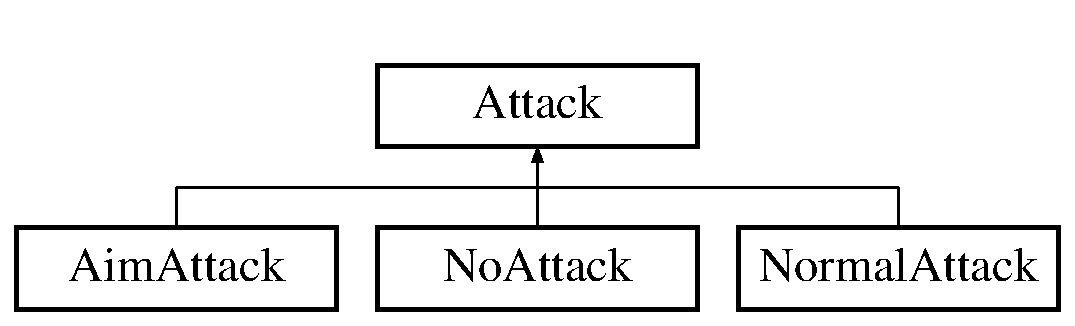
\includegraphics[height=2.000000cm]{class_attack}
\end{center}
\end{figure}
\subsection*{公開メンバ関数}
\begin{DoxyCompactItemize}
\item 
\hyperlink{class_attack_a7bfe78a7f5c0f41fad5e87f1cae7f6a5}{Attack} (int damage, int speed, int interval, \hyperlink{class_character}{Character} $\ast$chara)
\item 
void \hyperlink{class_attack_af2ea0dae02dde12d3fd31f10ceb374d0}{Do\+Attack} (\hyperlink{class_bullet}{Bullet} $\ast$bullet)
\item 
virtual void \hyperlink{class_attack_a06d145ff7c11cfef2b688eefcd11dac1}{Do\+Attack} ()=0
\item 
virtual void \hyperlink{class_attack_ac02b84493ca19adf8425c1ed2efaf54c}{Initialize\+Bullet} (int num)=0
\item 
void \hyperlink{class_attack_a60e57896cd31f3735746e2881f41f689}{Think\+Bullets} ()
\item 
void \hyperlink{class_attack_a82056bd6da4f30f961df75642cf6b2a6}{Draw\+Bullets} (int offset)
\item 
\hyperlink{class_attack_a178107a2b20a45b02adfdec72269711c}{$\sim$\+Attack} (void)
\item 
vector$<$ \hyperlink{class_bullet}{Bullet} $\ast$ $>$ \hyperlink{class_attack_ad6c6c719f3a56fafdf515394cc92869f}{bullets} ()
\item 
int \hyperlink{class_attack_aaa4045e8fe9f2ce9b3f473d3bf869c87}{Get\+Bullets\+Size} ()
\end{DoxyCompactItemize}
\subsection*{限定公開変数類}
\begin{DoxyCompactItemize}
\item 
vector$<$ \hyperlink{class_bullet}{Bullet} $\ast$ $>$ \hyperlink{class_attack_a4cacf753c3dd709aa9d09260f526213c}{bullets\+\_\+}
\item 
\hyperlink{class_character}{Character} $\ast$ \hyperlink{class_attack_a483c58b104388d57b0f9b380897a49c3}{chara\+\_\+}
\item 
int \hyperlink{class_attack_a2bfc44a2d532e0c38fa57c53e57e2995}{damage\+\_\+}
\item 
int \hyperlink{class_attack_a1baab21d135d9b9c7c4072b303c58963}{speed\+\_\+}
\item 
int \hyperlink{class_attack_a80bac689222ec4b3aa22691fe7b01380}{interval\+\_\+}
\item 
int \hyperlink{class_attack_a6fa9915c652fa7b30a80382b81cd9c1e}{interval\+\_\+count\+\_\+}
\end{DoxyCompactItemize}


\subsection{構築子と解体子}
\hypertarget{class_attack_a7bfe78a7f5c0f41fad5e87f1cae7f6a5}{\index{Attack@{Attack}!Attack@{Attack}}
\index{Attack@{Attack}!Attack@{Attack}}
\subsubsection[{Attack}]{\setlength{\rightskip}{0pt plus 5cm}Attack\+::\+Attack (
\begin{DoxyParamCaption}
\item[{int}]{damage, }
\item[{int}]{speed, }
\item[{int}]{interval, }
\item[{{\bf Character} $\ast$}]{chara}
\end{DoxyParamCaption}
)}}\label{class_attack_a7bfe78a7f5c0f41fad5e87f1cae7f6a5}
\hypertarget{class_attack_a178107a2b20a45b02adfdec72269711c}{\index{Attack@{Attack}!````~Attack@{$\sim$\+Attack}}
\index{````~Attack@{$\sim$\+Attack}!Attack@{Attack}}
\subsubsection[{$\sim$\+Attack}]{\setlength{\rightskip}{0pt plus 5cm}Attack\+::$\sim$\+Attack (
\begin{DoxyParamCaption}
\item[{void}]{}
\end{DoxyParamCaption}
)}}\label{class_attack_a178107a2b20a45b02adfdec72269711c}


\subsection{関数詳解}
\hypertarget{class_attack_ad6c6c719f3a56fafdf515394cc92869f}{\index{Attack@{Attack}!bullets@{bullets}}
\index{bullets@{bullets}!Attack@{Attack}}
\subsubsection[{bullets}]{\setlength{\rightskip}{0pt plus 5cm}vector$<${\bf Bullet}$\ast$$>$ Attack\+::bullets (
\begin{DoxyParamCaption}
{}
\end{DoxyParamCaption}
)\hspace{0.3cm}{\ttfamily [inline]}}}\label{class_attack_ad6c6c719f3a56fafdf515394cc92869f}
\hypertarget{class_attack_af2ea0dae02dde12d3fd31f10ceb374d0}{\index{Attack@{Attack}!Do\+Attack@{Do\+Attack}}
\index{Do\+Attack@{Do\+Attack}!Attack@{Attack}}
\subsubsection[{Do\+Attack}]{\setlength{\rightskip}{0pt plus 5cm}void Attack\+::\+Do\+Attack (
\begin{DoxyParamCaption}
\item[{{\bf Bullet} $\ast$}]{bullet}
\end{DoxyParamCaption}
)}}\label{class_attack_af2ea0dae02dde12d3fd31f10ceb374d0}
\hypertarget{class_attack_a06d145ff7c11cfef2b688eefcd11dac1}{\index{Attack@{Attack}!Do\+Attack@{Do\+Attack}}
\index{Do\+Attack@{Do\+Attack}!Attack@{Attack}}
\subsubsection[{Do\+Attack}]{\setlength{\rightskip}{0pt plus 5cm}virtual void Attack\+::\+Do\+Attack (
\begin{DoxyParamCaption}
{}
\end{DoxyParamCaption}
)\hspace{0.3cm}{\ttfamily [pure virtual]}}}\label{class_attack_a06d145ff7c11cfef2b688eefcd11dac1}


\hyperlink{class_aim_attack_abc5f35b870b83aecd372e5b3aef30b37}{Aim\+Attack}, \hyperlink{class_normal_attack_a39d8e90194dca1a89ba961163b7d0e18}{Normal\+Attack}, \hyperlink{class_no_attack_a42e89327c50ecc690056bf5c605a898b}{No\+Attack}で実装されています。

\hypertarget{class_attack_a82056bd6da4f30f961df75642cf6b2a6}{\index{Attack@{Attack}!Draw\+Bullets@{Draw\+Bullets}}
\index{Draw\+Bullets@{Draw\+Bullets}!Attack@{Attack}}
\subsubsection[{Draw\+Bullets}]{\setlength{\rightskip}{0pt plus 5cm}void Attack\+::\+Draw\+Bullets (
\begin{DoxyParamCaption}
\item[{int}]{offset}
\end{DoxyParamCaption}
)}}\label{class_attack_a82056bd6da4f30f961df75642cf6b2a6}
\hypertarget{class_attack_aaa4045e8fe9f2ce9b3f473d3bf869c87}{\index{Attack@{Attack}!Get\+Bullets\+Size@{Get\+Bullets\+Size}}
\index{Get\+Bullets\+Size@{Get\+Bullets\+Size}!Attack@{Attack}}
\subsubsection[{Get\+Bullets\+Size}]{\setlength{\rightskip}{0pt plus 5cm}int Attack\+::\+Get\+Bullets\+Size (
\begin{DoxyParamCaption}
{}
\end{DoxyParamCaption}
)}}\label{class_attack_aaa4045e8fe9f2ce9b3f473d3bf869c87}
\hypertarget{class_attack_ac02b84493ca19adf8425c1ed2efaf54c}{\index{Attack@{Attack}!Initialize\+Bullet@{Initialize\+Bullet}}
\index{Initialize\+Bullet@{Initialize\+Bullet}!Attack@{Attack}}
\subsubsection[{Initialize\+Bullet}]{\setlength{\rightskip}{0pt plus 5cm}virtual void Attack\+::\+Initialize\+Bullet (
\begin{DoxyParamCaption}
\item[{int}]{num}
\end{DoxyParamCaption}
)\hspace{0.3cm}{\ttfamily [pure virtual]}}}\label{class_attack_ac02b84493ca19adf8425c1ed2efaf54c}


\hyperlink{class_aim_attack_a965a7108493329d5d4b869e7289a3835}{Aim\+Attack}, \hyperlink{class_normal_attack_a95c5acd8739229d71395a8423c32a455}{Normal\+Attack}, \hyperlink{class_no_attack_a183ab68341fef13f86ea3ef020a53546}{No\+Attack}で実装されています。

\hypertarget{class_attack_a60e57896cd31f3735746e2881f41f689}{\index{Attack@{Attack}!Think\+Bullets@{Think\+Bullets}}
\index{Think\+Bullets@{Think\+Bullets}!Attack@{Attack}}
\subsubsection[{Think\+Bullets}]{\setlength{\rightskip}{0pt plus 5cm}void Attack\+::\+Think\+Bullets (
\begin{DoxyParamCaption}
{}
\end{DoxyParamCaption}
)}}\label{class_attack_a60e57896cd31f3735746e2881f41f689}


\subsection{メンバ詳解}
\hypertarget{class_attack_a4cacf753c3dd709aa9d09260f526213c}{\index{Attack@{Attack}!bullets\+\_\+@{bullets\+\_\+}}
\index{bullets\+\_\+@{bullets\+\_\+}!Attack@{Attack}}
\subsubsection[{bullets\+\_\+}]{\setlength{\rightskip}{0pt plus 5cm}vector$<${\bf Bullet}$\ast$$>$ Attack\+::bullets\+\_\+\hspace{0.3cm}{\ttfamily [protected]}}}\label{class_attack_a4cacf753c3dd709aa9d09260f526213c}
\hypertarget{class_attack_a483c58b104388d57b0f9b380897a49c3}{\index{Attack@{Attack}!chara\+\_\+@{chara\+\_\+}}
\index{chara\+\_\+@{chara\+\_\+}!Attack@{Attack}}
\subsubsection[{chara\+\_\+}]{\setlength{\rightskip}{0pt plus 5cm}{\bf Character}$\ast$ Attack\+::chara\+\_\+\hspace{0.3cm}{\ttfamily [protected]}}}\label{class_attack_a483c58b104388d57b0f9b380897a49c3}
\hypertarget{class_attack_a2bfc44a2d532e0c38fa57c53e57e2995}{\index{Attack@{Attack}!damage\+\_\+@{damage\+\_\+}}
\index{damage\+\_\+@{damage\+\_\+}!Attack@{Attack}}
\subsubsection[{damage\+\_\+}]{\setlength{\rightskip}{0pt plus 5cm}int Attack\+::damage\+\_\+\hspace{0.3cm}{\ttfamily [protected]}}}\label{class_attack_a2bfc44a2d532e0c38fa57c53e57e2995}
\hypertarget{class_attack_a80bac689222ec4b3aa22691fe7b01380}{\index{Attack@{Attack}!interval\+\_\+@{interval\+\_\+}}
\index{interval\+\_\+@{interval\+\_\+}!Attack@{Attack}}
\subsubsection[{interval\+\_\+}]{\setlength{\rightskip}{0pt plus 5cm}int Attack\+::interval\+\_\+\hspace{0.3cm}{\ttfamily [protected]}}}\label{class_attack_a80bac689222ec4b3aa22691fe7b01380}
\hypertarget{class_attack_a6fa9915c652fa7b30a80382b81cd9c1e}{\index{Attack@{Attack}!interval\+\_\+count\+\_\+@{interval\+\_\+count\+\_\+}}
\index{interval\+\_\+count\+\_\+@{interval\+\_\+count\+\_\+}!Attack@{Attack}}
\subsubsection[{interval\+\_\+count\+\_\+}]{\setlength{\rightskip}{0pt plus 5cm}int Attack\+::interval\+\_\+count\+\_\+\hspace{0.3cm}{\ttfamily [protected]}}}\label{class_attack_a6fa9915c652fa7b30a80382b81cd9c1e}
\hypertarget{class_attack_a1baab21d135d9b9c7c4072b303c58963}{\index{Attack@{Attack}!speed\+\_\+@{speed\+\_\+}}
\index{speed\+\_\+@{speed\+\_\+}!Attack@{Attack}}
\subsubsection[{speed\+\_\+}]{\setlength{\rightskip}{0pt plus 5cm}int Attack\+::speed\+\_\+\hspace{0.3cm}{\ttfamily [protected]}}}\label{class_attack_a1baab21d135d9b9c7c4072b303c58963}


このクラス詳解は次のファイルから抽出されました\+:\begin{DoxyCompactItemize}
\item 
\hyperlink{_attack_8h}{Attack.\+h}\item 
\hyperlink{_attack_8cpp}{Attack.\+cpp}\end{DoxyCompactItemize}

\hypertarget{class_bullet}{\section{Bullet クラス}
\label{class_bullet}\index{Bullet@{Bullet}}
}


{\ttfamily \#include $<$Bullet.\+h$>$}

Bullet の継承関係図\begin{figure}[H]
\begin{center}
\leavevmode
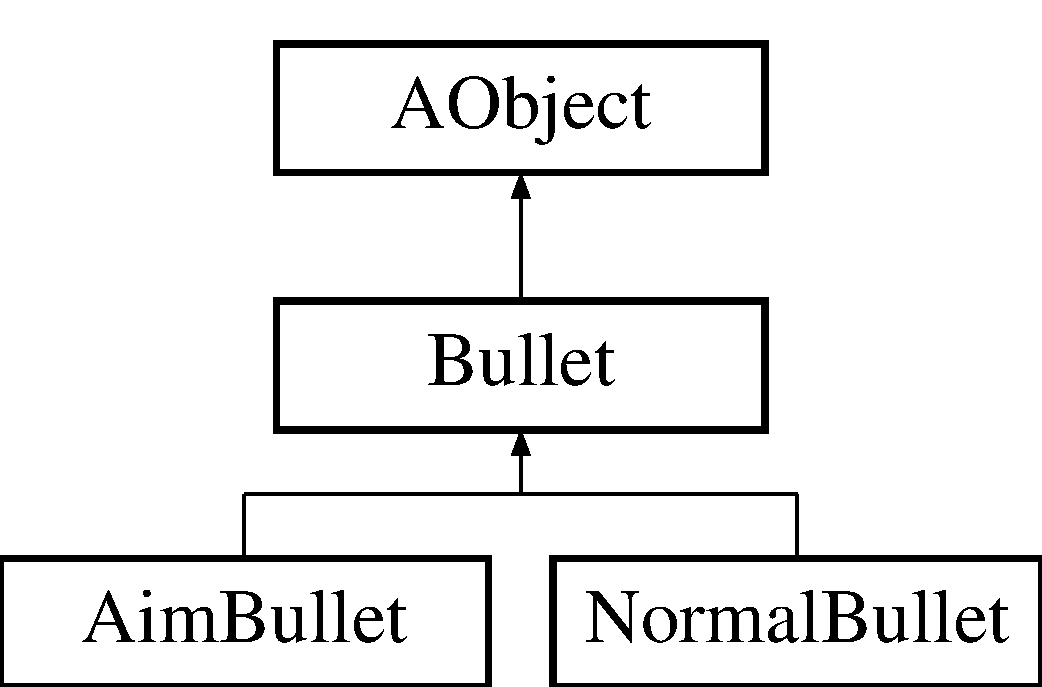
\includegraphics[height=3.000000cm]{class_bullet}
\end{center}
\end{figure}
\subsection*{公開メンバ関数}
\begin{DoxyCompactItemize}
\item 
\hyperlink{class_bullet_a62798f15ff62617a274c12ad1ffb9aad}{Bullet} (double x, double y, int \hyperlink{class_bullet_a6e5b78574ec8fbff411b1319cf111799}{damage}, int \hyperlink{class_a_object_abb924b7e558a2f9d86f2db2bc2fb18a4}{speed}, char $\ast$fname, int hit\+\_\+size\+\_\+x, int hit\+\_\+size\+\_\+y)
\item 
virtual void \hyperlink{class_bullet_a0f3207f4dc7244fd3510b89943f939f3}{Think} ()
\item 
void \hyperlink{class_bullet_a67b44c96157279508e92f9dc91419f38}{Die\+Bullet} ()
\item 
virtual void \hyperlink{class_bullet_a4c20c48e68e8b14c9df456c50f61998d}{Initialize} (double x, double y)
\item 
\hyperlink{class_bullet_ab3c2b9c0b12c18aeace52bd289ddfce3}{$\sim$\+Bullet} (void)
\item 
int \hyperlink{class_bullet_a6e5b78574ec8fbff411b1319cf111799}{damage} ()
\end{DoxyCompactItemize}
\subsection*{限定公開変数類}
\begin{DoxyCompactItemize}
\item 
int \hyperlink{class_bullet_aaa26f3bff8a6f418831cf7458e018b40}{damage\+\_\+}
\item 
int \hyperlink{class_bullet_aff48665a8060391eaca9bb2d38b8492f}{bullet\+\_\+speed\+\_\+}
\item 
double \hyperlink{class_bullet_a70eee9d25fde596eb251251e3806a6cc}{angle\+\_\+}
\end{DoxyCompactItemize}
\subsection*{その他の継承メンバ}


\subsection{構築子と解体子}
\hypertarget{class_bullet_a62798f15ff62617a274c12ad1ffb9aad}{\index{Bullet@{Bullet}!Bullet@{Bullet}}
\index{Bullet@{Bullet}!Bullet@{Bullet}}
\subsubsection[{Bullet}]{\setlength{\rightskip}{0pt plus 5cm}Bullet\+::\+Bullet (
\begin{DoxyParamCaption}
\item[{double}]{x, }
\item[{double}]{y, }
\item[{int}]{damage, }
\item[{int}]{speed, }
\item[{char $\ast$}]{fname, }
\item[{int}]{hit\+\_\+size\+\_\+x, }
\item[{int}]{hit\+\_\+size\+\_\+y}
\end{DoxyParamCaption}
)}}\label{class_bullet_a62798f15ff62617a274c12ad1ffb9aad}
\hypertarget{class_bullet_ab3c2b9c0b12c18aeace52bd289ddfce3}{\index{Bullet@{Bullet}!````~Bullet@{$\sim$\+Bullet}}
\index{````~Bullet@{$\sim$\+Bullet}!Bullet@{Bullet}}
\subsubsection[{$\sim$\+Bullet}]{\setlength{\rightskip}{0pt plus 5cm}Bullet\+::$\sim$\+Bullet (
\begin{DoxyParamCaption}
\item[{void}]{}
\end{DoxyParamCaption}
)}}\label{class_bullet_ab3c2b9c0b12c18aeace52bd289ddfce3}


\subsection{関数詳解}
\hypertarget{class_bullet_a6e5b78574ec8fbff411b1319cf111799}{\index{Bullet@{Bullet}!damage@{damage}}
\index{damage@{damage}!Bullet@{Bullet}}
\subsubsection[{damage}]{\setlength{\rightskip}{0pt plus 5cm}int Bullet\+::damage (
\begin{DoxyParamCaption}
{}
\end{DoxyParamCaption}
)\hspace{0.3cm}{\ttfamily [inline]}}}\label{class_bullet_a6e5b78574ec8fbff411b1319cf111799}
\hypertarget{class_bullet_a67b44c96157279508e92f9dc91419f38}{\index{Bullet@{Bullet}!Die\+Bullet@{Die\+Bullet}}
\index{Die\+Bullet@{Die\+Bullet}!Bullet@{Bullet}}
\subsubsection[{Die\+Bullet}]{\setlength{\rightskip}{0pt plus 5cm}void Bullet\+::\+Die\+Bullet (
\begin{DoxyParamCaption}
{}
\end{DoxyParamCaption}
)}}\label{class_bullet_a67b44c96157279508e92f9dc91419f38}
\hypertarget{class_bullet_a4c20c48e68e8b14c9df456c50f61998d}{\index{Bullet@{Bullet}!Initialize@{Initialize}}
\index{Initialize@{Initialize}!Bullet@{Bullet}}
\subsubsection[{Initialize}]{\setlength{\rightskip}{0pt plus 5cm}void Bullet\+::\+Initialize (
\begin{DoxyParamCaption}
\item[{double}]{x, }
\item[{double}]{y}
\end{DoxyParamCaption}
)\hspace{0.3cm}{\ttfamily [virtual]}}}\label{class_bullet_a4c20c48e68e8b14c9df456c50f61998d}
\hypertarget{class_bullet_a0f3207f4dc7244fd3510b89943f939f3}{\index{Bullet@{Bullet}!Think@{Think}}
\index{Think@{Think}!Bullet@{Bullet}}
\subsubsection[{Think}]{\setlength{\rightskip}{0pt plus 5cm}void Bullet\+::\+Think (
\begin{DoxyParamCaption}
{}
\end{DoxyParamCaption}
)\hspace{0.3cm}{\ttfamily [virtual]}}}\label{class_bullet_a0f3207f4dc7244fd3510b89943f939f3}


\hyperlink{class_a_object_a61f89197cb14b1270a0a232ee88333a0}{A\+Object}を実装しています。



\subsection{メンバ詳解}
\hypertarget{class_bullet_a70eee9d25fde596eb251251e3806a6cc}{\index{Bullet@{Bullet}!angle\+\_\+@{angle\+\_\+}}
\index{angle\+\_\+@{angle\+\_\+}!Bullet@{Bullet}}
\subsubsection[{angle\+\_\+}]{\setlength{\rightskip}{0pt plus 5cm}double Bullet\+::angle\+\_\+\hspace{0.3cm}{\ttfamily [protected]}}}\label{class_bullet_a70eee9d25fde596eb251251e3806a6cc}
\hypertarget{class_bullet_aff48665a8060391eaca9bb2d38b8492f}{\index{Bullet@{Bullet}!bullet\+\_\+speed\+\_\+@{bullet\+\_\+speed\+\_\+}}
\index{bullet\+\_\+speed\+\_\+@{bullet\+\_\+speed\+\_\+}!Bullet@{Bullet}}
\subsubsection[{bullet\+\_\+speed\+\_\+}]{\setlength{\rightskip}{0pt plus 5cm}int Bullet\+::bullet\+\_\+speed\+\_\+\hspace{0.3cm}{\ttfamily [protected]}}}\label{class_bullet_aff48665a8060391eaca9bb2d38b8492f}
\hypertarget{class_bullet_aaa26f3bff8a6f418831cf7458e018b40}{\index{Bullet@{Bullet}!damage\+\_\+@{damage\+\_\+}}
\index{damage\+\_\+@{damage\+\_\+}!Bullet@{Bullet}}
\subsubsection[{damage\+\_\+}]{\setlength{\rightskip}{0pt plus 5cm}int Bullet\+::damage\+\_\+\hspace{0.3cm}{\ttfamily [protected]}}}\label{class_bullet_aaa26f3bff8a6f418831cf7458e018b40}


このクラス詳解は次のファイルから抽出されました\+:\begin{DoxyCompactItemize}
\item 
\hyperlink{_bullet_8h}{Bullet.\+h}\item 
\hyperlink{_bullet_8cpp}{Bullet.\+cpp}\end{DoxyCompactItemize}

\hypertarget{class_character}{\section{Character クラス}
\label{class_character}\index{Character@{Character}}
}


{\ttfamily \#include $<$Character.\+h$>$}

Character の継承関係図\begin{figure}[H]
\begin{center}
\leavevmode
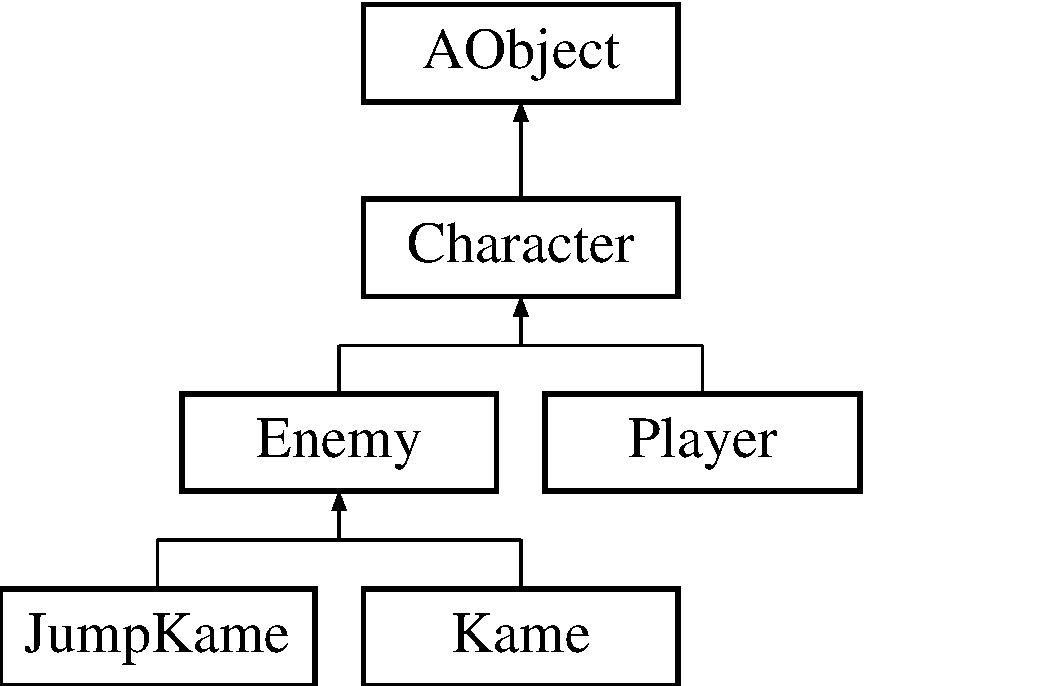
\includegraphics[height=4.000000cm]{class_character}
\end{center}
\end{figure}
\subsection*{公開メンバ関数}
\begin{DoxyCompactItemize}
\item 
\hyperlink{class_character_a6c56f5d53bfe5f5a194e2329fdae3abd}{Character} (double x, double y, int \hyperlink{class_character_a7ea1356e63b9c74e9568feec5e1c92f5}{hp}, char $\ast$f\+\_\+name, int size\+\_\+x, int size\+\_\+y, bool \hyperlink{class_a_object_a7453abe76bbddf446aa5787231428a52}{right}, \hyperlink{class_character_controller}{Character\+Controller} $\ast$controller, \hyperlink{class_attack}{Attack} $\ast$attack)
\item 
virtual void \hyperlink{class_character_a7622bdde334c8d37358218e64dd6850a}{Jump} ()
\item 
virtual void \hyperlink{class_character_a011928a158278ccaa7129514e54ce933}{Walk} (bool \hyperlink{class_a_object_a7453abe76bbddf446aa5787231428a52}{right})
\item 
virtual void \hyperlink{class_character_a8b16b07f609409c077680199b6c50ae1}{Run} (bool \hyperlink{class_a_object_a7453abe76bbddf446aa5787231428a52}{right})
\item 
void \hyperlink{class_character_a98038fd0e31c18a4d7ca5a147db30ae1}{No\+Move} ()
\item 
void \hyperlink{class_character_a97406a1d787de885f5c54b3f21fc9b89}{Do\+Attack} ()
\item 
void \hyperlink{class_character_a99682c871c2120789442f3201b257ad1}{Damaged} (int damage)
\item 
void \hyperlink{class_character_a953e7c76dce887426f74e568e5ebbe39}{Think} ()
\item 
vector$<$ \hyperlink{class_bullet}{Bullet} $\ast$ $>$ \hyperlink{class_character_abd9a81f598e6daeefaaf68cedb706481}{Get\+Bullets} ()
\item 
int \hyperlink{class_character_a7ea1356e63b9c74e9568feec5e1c92f5}{hp} ()
\item 
int \hyperlink{class_character_a1e9966d232a386c7f9cc01db9e31fc23}{max\+Hp} ()
\item 
int \hyperlink{class_character_a13eec960e58d54403e6babfa6caa11a1}{Get\+Bullets\+Size} ()
\item 
void \hyperlink{class_character_a6c1fa20d22b5ea6edc4dbd6ca9496411}{Reset} ()
\item 
virtual void \hyperlink{class_character_ad359a991510783008ee96060f247c990}{Draw} (int offset)
\end{DoxyCompactItemize}
\subsection*{限定公開変数類}
\begin{DoxyCompactItemize}
\item 
int \hyperlink{class_character_a9434f06db3acc96bb5646a0f287c3692}{hp\+\_\+}
\item 
int \hyperlink{class_character_a38ef78d8db07674b25dfd360b4d6415e}{max\+\_\+hp\+\_\+}
\item 
int \hyperlink{class_character_aa27916b9cbe1108d86c3e43f64afc0f9}{status\+\_\+}
\item 
\hyperlink{class_character_controller}{Character\+Controller} $\ast$ \hyperlink{class_character_ac2aa119a9bef3db8ca9bbed9040ad6d2}{controller\+\_\+}
\item 
\hyperlink{class_attack}{Attack} $\ast$ \hyperlink{class_character_a54a04aba4002a2ca97e4b26f2d134d55}{attack\+\_\+}
\end{DoxyCompactItemize}
\subsection*{その他の継承メンバ}


\subsection{構築子と解体子}
\hypertarget{class_character_a6c56f5d53bfe5f5a194e2329fdae3abd}{\index{Character@{Character}!Character@{Character}}
\index{Character@{Character}!Character@{Character}}
\subsubsection[{Character}]{\setlength{\rightskip}{0pt plus 5cm}Character\+::\+Character (
\begin{DoxyParamCaption}
\item[{double}]{x, }
\item[{double}]{y, }
\item[{int}]{hp, }
\item[{char $\ast$}]{f\+\_\+name, }
\item[{int}]{size\+\_\+x, }
\item[{int}]{size\+\_\+y, }
\item[{bool}]{right, }
\item[{{\bf Character\+Controller} $\ast$}]{controller, }
\item[{{\bf Attack} $\ast$}]{attack}
\end{DoxyParamCaption}
)}}\label{class_character_a6c56f5d53bfe5f5a194e2329fdae3abd}


\subsection{関数詳解}
\hypertarget{class_character_a99682c871c2120789442f3201b257ad1}{\index{Character@{Character}!Damaged@{Damaged}}
\index{Damaged@{Damaged}!Character@{Character}}
\subsubsection[{Damaged}]{\setlength{\rightskip}{0pt plus 5cm}void Character\+::\+Damaged (
\begin{DoxyParamCaption}
\item[{int}]{damage}
\end{DoxyParamCaption}
)}}\label{class_character_a99682c871c2120789442f3201b257ad1}
\hypertarget{class_character_a97406a1d787de885f5c54b3f21fc9b89}{\index{Character@{Character}!Do\+Attack@{Do\+Attack}}
\index{Do\+Attack@{Do\+Attack}!Character@{Character}}
\subsubsection[{Do\+Attack}]{\setlength{\rightskip}{0pt plus 5cm}void Character\+::\+Do\+Attack (
\begin{DoxyParamCaption}
{}
\end{DoxyParamCaption}
)}}\label{class_character_a97406a1d787de885f5c54b3f21fc9b89}
\hypertarget{class_character_ad359a991510783008ee96060f247c990}{\index{Character@{Character}!Draw@{Draw}}
\index{Draw@{Draw}!Character@{Character}}
\subsubsection[{Draw}]{\setlength{\rightskip}{0pt plus 5cm}void Character\+::\+Draw (
\begin{DoxyParamCaption}
\item[{int}]{offset}
\end{DoxyParamCaption}
)\hspace{0.3cm}{\ttfamily [virtual]}}}\label{class_character_ad359a991510783008ee96060f247c990}


\hyperlink{class_a_object_a0e279a93c79be5807e9bbd20875369a2}{A\+Object}を再実装しています。



\hyperlink{class_player_a5e32dec9258cfa8145e482fed4c42c83}{Player}で再実装されています。

\hypertarget{class_character_abd9a81f598e6daeefaaf68cedb706481}{\index{Character@{Character}!Get\+Bullets@{Get\+Bullets}}
\index{Get\+Bullets@{Get\+Bullets}!Character@{Character}}
\subsubsection[{Get\+Bullets}]{\setlength{\rightskip}{0pt plus 5cm}vector$<$ {\bf Bullet} $\ast$ $>$ Character\+::\+Get\+Bullets (
\begin{DoxyParamCaption}
{}
\end{DoxyParamCaption}
)}}\label{class_character_abd9a81f598e6daeefaaf68cedb706481}
\hypertarget{class_character_a13eec960e58d54403e6babfa6caa11a1}{\index{Character@{Character}!Get\+Bullets\+Size@{Get\+Bullets\+Size}}
\index{Get\+Bullets\+Size@{Get\+Bullets\+Size}!Character@{Character}}
\subsubsection[{Get\+Bullets\+Size}]{\setlength{\rightskip}{0pt plus 5cm}int Character\+::\+Get\+Bullets\+Size (
\begin{DoxyParamCaption}
{}
\end{DoxyParamCaption}
)\hspace{0.3cm}{\ttfamily [inline]}}}\label{class_character_a13eec960e58d54403e6babfa6caa11a1}
\hypertarget{class_character_a7ea1356e63b9c74e9568feec5e1c92f5}{\index{Character@{Character}!hp@{hp}}
\index{hp@{hp}!Character@{Character}}
\subsubsection[{hp}]{\setlength{\rightskip}{0pt plus 5cm}int Character\+::hp (
\begin{DoxyParamCaption}
{}
\end{DoxyParamCaption}
)\hspace{0.3cm}{\ttfamily [inline]}}}\label{class_character_a7ea1356e63b9c74e9568feec5e1c92f5}
\hypertarget{class_character_a7622bdde334c8d37358218e64dd6850a}{\index{Character@{Character}!Jump@{Jump}}
\index{Jump@{Jump}!Character@{Character}}
\subsubsection[{Jump}]{\setlength{\rightskip}{0pt plus 5cm}void Character\+::\+Jump (
\begin{DoxyParamCaption}
{}
\end{DoxyParamCaption}
)\hspace{0.3cm}{\ttfamily [virtual]}}}\label{class_character_a7622bdde334c8d37358218e64dd6850a}


\hyperlink{class_player_a1334990b8b7aaaad904e22f03f4d947d}{Player}, \hyperlink{class_jump_kame_a0875bf1b86766d23294c754b63f56a0c}{Jump\+Kame}で再実装されています。

\hypertarget{class_character_a1e9966d232a386c7f9cc01db9e31fc23}{\index{Character@{Character}!max\+Hp@{max\+Hp}}
\index{max\+Hp@{max\+Hp}!Character@{Character}}
\subsubsection[{max\+Hp}]{\setlength{\rightskip}{0pt plus 5cm}int Character\+::max\+Hp (
\begin{DoxyParamCaption}
{}
\end{DoxyParamCaption}
)\hspace{0.3cm}{\ttfamily [inline]}}}\label{class_character_a1e9966d232a386c7f9cc01db9e31fc23}
\hypertarget{class_character_a98038fd0e31c18a4d7ca5a147db30ae1}{\index{Character@{Character}!No\+Move@{No\+Move}}
\index{No\+Move@{No\+Move}!Character@{Character}}
\subsubsection[{No\+Move}]{\setlength{\rightskip}{0pt plus 5cm}void Character\+::\+No\+Move (
\begin{DoxyParamCaption}
{}
\end{DoxyParamCaption}
)}}\label{class_character_a98038fd0e31c18a4d7ca5a147db30ae1}
\hypertarget{class_character_a6c1fa20d22b5ea6edc4dbd6ca9496411}{\index{Character@{Character}!Reset@{Reset}}
\index{Reset@{Reset}!Character@{Character}}
\subsubsection[{Reset}]{\setlength{\rightskip}{0pt plus 5cm}void Character\+::\+Reset (
\begin{DoxyParamCaption}
{}
\end{DoxyParamCaption}
)\hspace{0.3cm}{\ttfamily [virtual]}}}\label{class_character_a6c1fa20d22b5ea6edc4dbd6ca9496411}


\hyperlink{class_a_object_aa07f4874e508e22cc0980e5ab6eb7f54}{A\+Object}を再実装しています。



\hyperlink{class_player_a22a0d2b901622c497b677b7c75fafe45}{Player}で再実装されています。

\hypertarget{class_character_a8b16b07f609409c077680199b6c50ae1}{\index{Character@{Character}!Run@{Run}}
\index{Run@{Run}!Character@{Character}}
\subsubsection[{Run}]{\setlength{\rightskip}{0pt plus 5cm}void Character\+::\+Run (
\begin{DoxyParamCaption}
\item[{bool}]{right}
\end{DoxyParamCaption}
)\hspace{0.3cm}{\ttfamily [virtual]}}}\label{class_character_a8b16b07f609409c077680199b6c50ae1}
\hypertarget{class_character_a953e7c76dce887426f74e568e5ebbe39}{\index{Character@{Character}!Think@{Think}}
\index{Think@{Think}!Character@{Character}}
\subsubsection[{Think}]{\setlength{\rightskip}{0pt plus 5cm}void Character\+::\+Think (
\begin{DoxyParamCaption}
{}
\end{DoxyParamCaption}
)\hspace{0.3cm}{\ttfamily [virtual]}}}\label{class_character_a953e7c76dce887426f74e568e5ebbe39}


\hyperlink{class_a_object_a61f89197cb14b1270a0a232ee88333a0}{A\+Object}を実装しています。

\hypertarget{class_character_a011928a158278ccaa7129514e54ce933}{\index{Character@{Character}!Walk@{Walk}}
\index{Walk@{Walk}!Character@{Character}}
\subsubsection[{Walk}]{\setlength{\rightskip}{0pt plus 5cm}void Character\+::\+Walk (
\begin{DoxyParamCaption}
\item[{bool}]{right}
\end{DoxyParamCaption}
)\hspace{0.3cm}{\ttfamily [virtual]}}}\label{class_character_a011928a158278ccaa7129514e54ce933}


\subsection{メンバ詳解}
\hypertarget{class_character_a54a04aba4002a2ca97e4b26f2d134d55}{\index{Character@{Character}!attack\+\_\+@{attack\+\_\+}}
\index{attack\+\_\+@{attack\+\_\+}!Character@{Character}}
\subsubsection[{attack\+\_\+}]{\setlength{\rightskip}{0pt plus 5cm}{\bf Attack}$\ast$ Character\+::attack\+\_\+\hspace{0.3cm}{\ttfamily [protected]}}}\label{class_character_a54a04aba4002a2ca97e4b26f2d134d55}
\hypertarget{class_character_ac2aa119a9bef3db8ca9bbed9040ad6d2}{\index{Character@{Character}!controller\+\_\+@{controller\+\_\+}}
\index{controller\+\_\+@{controller\+\_\+}!Character@{Character}}
\subsubsection[{controller\+\_\+}]{\setlength{\rightskip}{0pt plus 5cm}{\bf Character\+Controller}$\ast$ Character\+::controller\+\_\+\hspace{0.3cm}{\ttfamily [protected]}}}\label{class_character_ac2aa119a9bef3db8ca9bbed9040ad6d2}
\hypertarget{class_character_a9434f06db3acc96bb5646a0f287c3692}{\index{Character@{Character}!hp\+\_\+@{hp\+\_\+}}
\index{hp\+\_\+@{hp\+\_\+}!Character@{Character}}
\subsubsection[{hp\+\_\+}]{\setlength{\rightskip}{0pt plus 5cm}int Character\+::hp\+\_\+\hspace{0.3cm}{\ttfamily [protected]}}}\label{class_character_a9434f06db3acc96bb5646a0f287c3692}
\hypertarget{class_character_a38ef78d8db07674b25dfd360b4d6415e}{\index{Character@{Character}!max\+\_\+hp\+\_\+@{max\+\_\+hp\+\_\+}}
\index{max\+\_\+hp\+\_\+@{max\+\_\+hp\+\_\+}!Character@{Character}}
\subsubsection[{max\+\_\+hp\+\_\+}]{\setlength{\rightskip}{0pt plus 5cm}int Character\+::max\+\_\+hp\+\_\+\hspace{0.3cm}{\ttfamily [protected]}}}\label{class_character_a38ef78d8db07674b25dfd360b4d6415e}
\hypertarget{class_character_aa27916b9cbe1108d86c3e43f64afc0f9}{\index{Character@{Character}!status\+\_\+@{status\+\_\+}}
\index{status\+\_\+@{status\+\_\+}!Character@{Character}}
\subsubsection[{status\+\_\+}]{\setlength{\rightskip}{0pt plus 5cm}int Character\+::status\+\_\+\hspace{0.3cm}{\ttfamily [protected]}}}\label{class_character_aa27916b9cbe1108d86c3e43f64afc0f9}


このクラス詳解は次のファイルから抽出されました\+:\begin{DoxyCompactItemize}
\item 
\hyperlink{_character_8h}{Character.\+h}\item 
\hyperlink{_character_8cpp}{Character.\+cpp}\end{DoxyCompactItemize}

\hypertarget{class_character_controller}{\section{Character\+Controller クラス}
\label{class_character_controller}\index{Character\+Controller@{Character\+Controller}}
}


{\ttfamily \#include $<$Character\+Controller.\+h$>$}

Character\+Controller の継承関係図\begin{figure}[H]
\begin{center}
\leavevmode
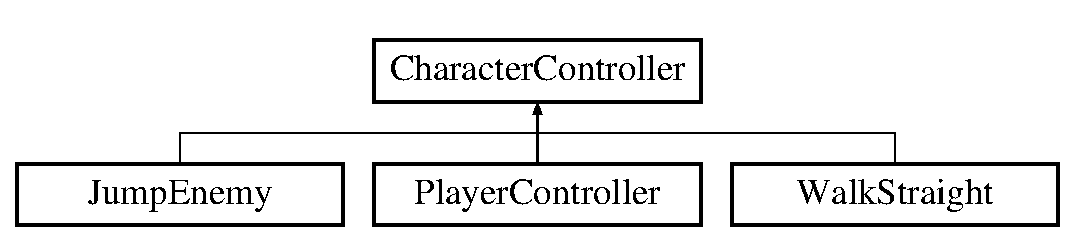
\includegraphics[height=2.000000cm]{class_character_controller}
\end{center}
\end{figure}
\subsection*{公開メンバ関数}
\begin{DoxyCompactItemize}
\item 
\hyperlink{class_character_controller_a7f5914352c01a47e1a4ac75e3e277caa}{Character\+Controller} ()
\item 
\hyperlink{class_character_controller_a8c29d02e93455dd56828ae451769c53a}{Character\+Controller} (\hyperlink{class_character}{Character} $\ast$character, \hyperlink{class_field}{Field} $\ast$field)
\item 
virtual void \hyperlink{class_character_controller_a493d5b59610546133900f4de7110a487}{Think} ()=0
\end{DoxyCompactItemize}
\subsection*{限定公開変数類}
\begin{DoxyCompactItemize}
\item 
\hyperlink{class_character}{Character} $\ast$ \hyperlink{class_character_controller_a41167a323fafc09685765780911eab13}{character\+\_\+}
\item 
\hyperlink{class_field}{Field} $\ast$ \hyperlink{class_character_controller_aee517c96b5c50a91aa1b0f16b8defd01}{field\+\_\+}
\end{DoxyCompactItemize}


\subsection{構築子と解体子}
\hypertarget{class_character_controller_a7f5914352c01a47e1a4ac75e3e277caa}{\index{Character\+Controller@{Character\+Controller}!Character\+Controller@{Character\+Controller}}
\index{Character\+Controller@{Character\+Controller}!Character\+Controller@{Character\+Controller}}
\subsubsection[{Character\+Controller}]{\setlength{\rightskip}{0pt plus 5cm}Character\+Controller\+::\+Character\+Controller (
\begin{DoxyParamCaption}
{}
\end{DoxyParamCaption}
)}}\label{class_character_controller_a7f5914352c01a47e1a4ac75e3e277caa}
\hypertarget{class_character_controller_a8c29d02e93455dd56828ae451769c53a}{\index{Character\+Controller@{Character\+Controller}!Character\+Controller@{Character\+Controller}}
\index{Character\+Controller@{Character\+Controller}!Character\+Controller@{Character\+Controller}}
\subsubsection[{Character\+Controller}]{\setlength{\rightskip}{0pt plus 5cm}Character\+Controller\+::\+Character\+Controller (
\begin{DoxyParamCaption}
\item[{{\bf Character} $\ast$}]{character, }
\item[{{\bf Field} $\ast$}]{field}
\end{DoxyParamCaption}
)}}\label{class_character_controller_a8c29d02e93455dd56828ae451769c53a}


\subsection{関数詳解}
\hypertarget{class_character_controller_a493d5b59610546133900f4de7110a487}{\index{Character\+Controller@{Character\+Controller}!Think@{Think}}
\index{Think@{Think}!Character\+Controller@{Character\+Controller}}
\subsubsection[{Think}]{\setlength{\rightskip}{0pt plus 5cm}virtual void Character\+Controller\+::\+Think (
\begin{DoxyParamCaption}
{}
\end{DoxyParamCaption}
)\hspace{0.3cm}{\ttfamily [pure virtual]}}}\label{class_character_controller_a493d5b59610546133900f4de7110a487}


\hyperlink{class_player_controller_a3331f219d6f6a735c1e6cda5e8abb298}{Player\+Controller}, \hyperlink{class_jump_enemy_abd7019f8b333e710c1bb65b1b599182c}{Jump\+Enemy}, \hyperlink{class_walk_straight_ad8a6f6a0947df875c253752f72e9af0f}{Walk\+Straight}で実装されています。



\subsection{メンバ詳解}
\hypertarget{class_character_controller_a41167a323fafc09685765780911eab13}{\index{Character\+Controller@{Character\+Controller}!character\+\_\+@{character\+\_\+}}
\index{character\+\_\+@{character\+\_\+}!Character\+Controller@{Character\+Controller}}
\subsubsection[{character\+\_\+}]{\setlength{\rightskip}{0pt plus 5cm}{\bf Character}$\ast$ Character\+Controller\+::character\+\_\+\hspace{0.3cm}{\ttfamily [protected]}}}\label{class_character_controller_a41167a323fafc09685765780911eab13}
\hypertarget{class_character_controller_aee517c96b5c50a91aa1b0f16b8defd01}{\index{Character\+Controller@{Character\+Controller}!field\+\_\+@{field\+\_\+}}
\index{field\+\_\+@{field\+\_\+}!Character\+Controller@{Character\+Controller}}
\subsubsection[{field\+\_\+}]{\setlength{\rightskip}{0pt plus 5cm}{\bf Field}$\ast$ Character\+Controller\+::field\+\_\+\hspace{0.3cm}{\ttfamily [protected]}}}\label{class_character_controller_aee517c96b5c50a91aa1b0f16b8defd01}


このクラス詳解は次のファイルから抽出されました\+:\begin{DoxyCompactItemize}
\item 
\hyperlink{_character_controller_8h}{Character\+Controller.\+h}\item 
\hyperlink{_character_controller_8cpp}{Character\+Controller.\+cpp}\end{DoxyCompactItemize}

\hypertarget{class_coin}{\section{Coin クラス}
\label{class_coin}\index{Coin@{Coin}}
}


{\ttfamily \#include $<$Coin.\+h$>$}

Coin の継承関係図\begin{figure}[H]
\begin{center}
\leavevmode
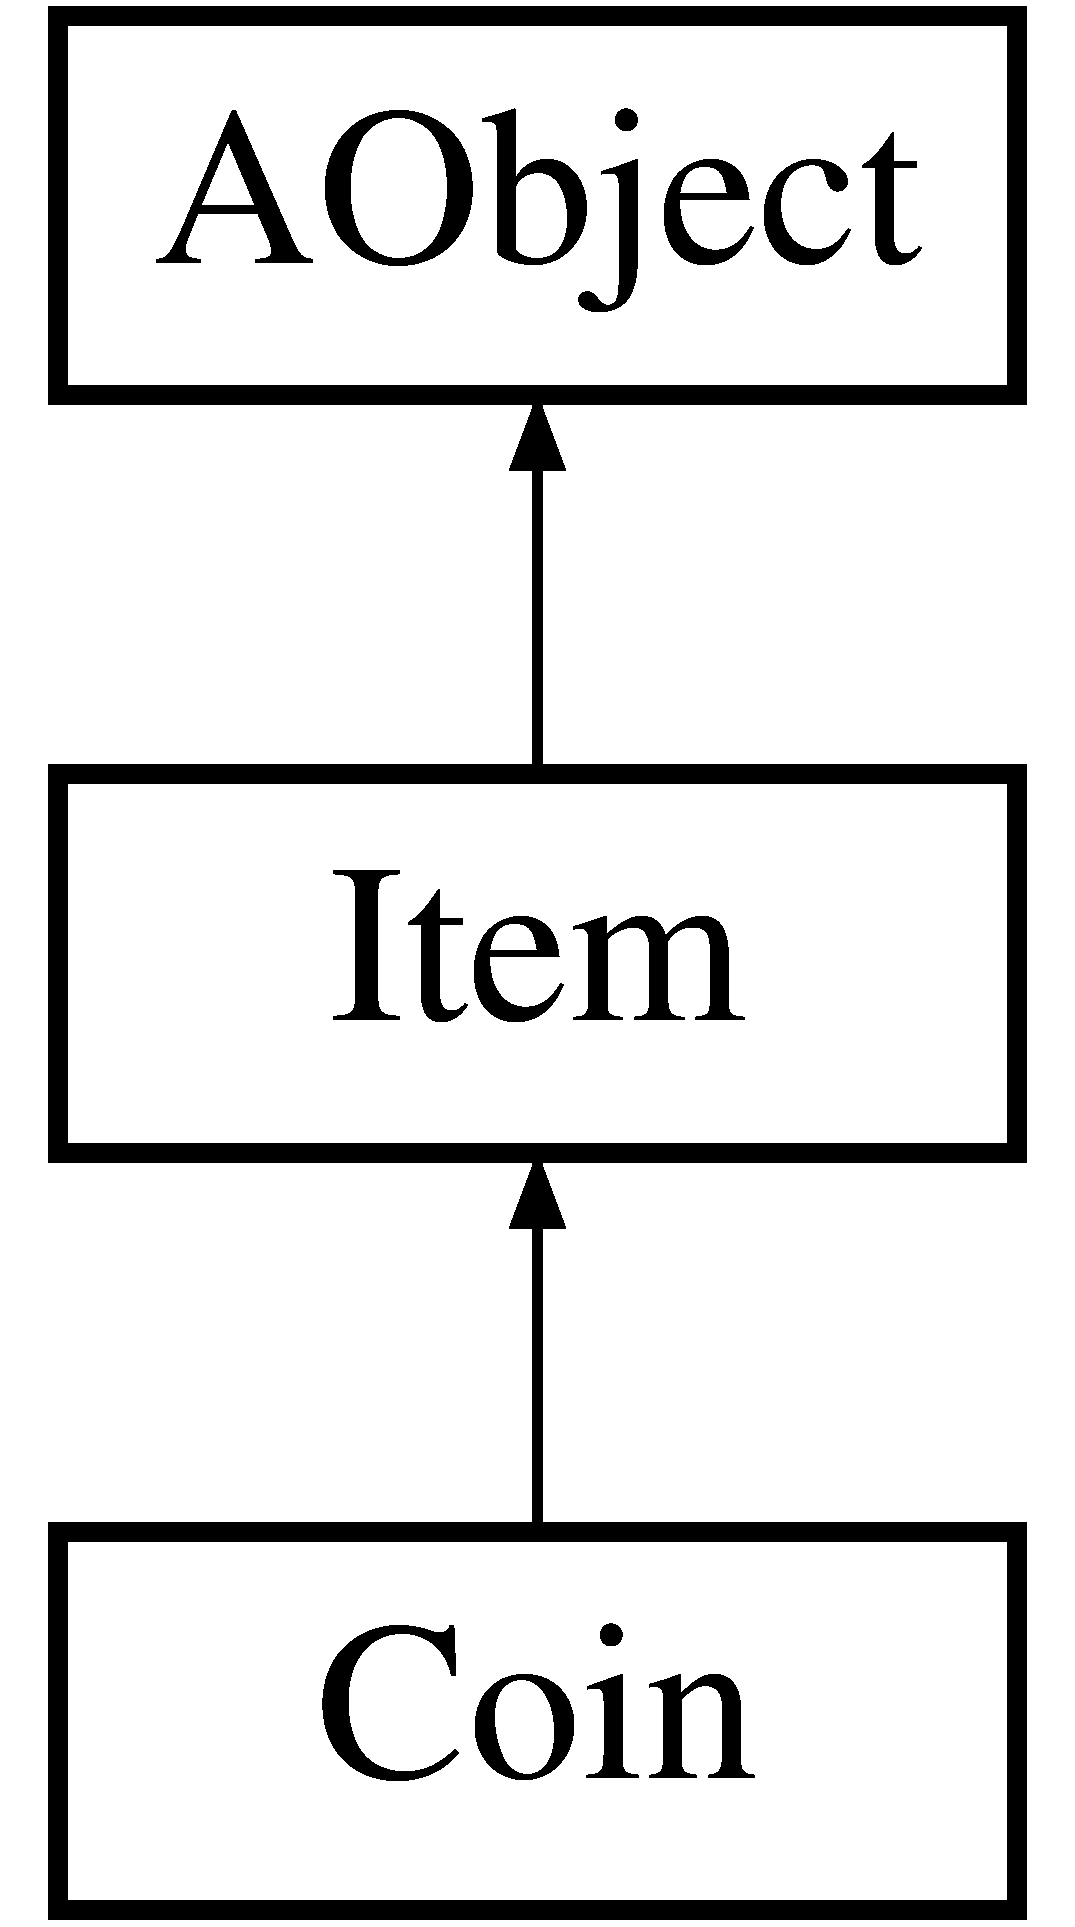
\includegraphics[height=3.000000cm]{class_coin}
\end{center}
\end{figure}
\subsection*{公開メンバ関数}
\begin{DoxyCompactItemize}
\item 
\hyperlink{class_coin_a0775a82e2aaf83ad15cf0495ec688b5a}{Coin} (double ax, double ay)
\item 
void \hyperlink{class_coin_a6991c98735397b008309f713a252d2cd}{Affect} (\hyperlink{class_character}{Character} $\ast$character)
\item 
void \hyperlink{class_coin_a3bfc309bcea6da0bda2913ffc20adbdd}{Think} ()
\end{DoxyCompactItemize}
\subsection*{その他の継承メンバ}


\subsection{構築子と解体子}
\hypertarget{class_coin_a0775a82e2aaf83ad15cf0495ec688b5a}{\index{Coin@{Coin}!Coin@{Coin}}
\index{Coin@{Coin}!Coin@{Coin}}
\subsubsection[{Coin}]{\setlength{\rightskip}{0pt plus 5cm}Coin\+::\+Coin (
\begin{DoxyParamCaption}
\item[{double}]{ax, }
\item[{double}]{ay}
\end{DoxyParamCaption}
)}}\label{class_coin_a0775a82e2aaf83ad15cf0495ec688b5a}


\subsection{関数詳解}
\hypertarget{class_coin_a6991c98735397b008309f713a252d2cd}{\index{Coin@{Coin}!Affect@{Affect}}
\index{Affect@{Affect}!Coin@{Coin}}
\subsubsection[{Affect}]{\setlength{\rightskip}{0pt plus 5cm}void Coin\+::\+Affect (
\begin{DoxyParamCaption}
\item[{{\bf Character} $\ast$}]{character}
\end{DoxyParamCaption}
)\hspace{0.3cm}{\ttfamily [virtual]}}}\label{class_coin_a6991c98735397b008309f713a252d2cd}


\hyperlink{class_item_a3102747c3c78a04691d821d1be363354}{Item}を実装しています。

\hypertarget{class_coin_a3bfc309bcea6da0bda2913ffc20adbdd}{\index{Coin@{Coin}!Think@{Think}}
\index{Think@{Think}!Coin@{Coin}}
\subsubsection[{Think}]{\setlength{\rightskip}{0pt plus 5cm}void Coin\+::\+Think (
\begin{DoxyParamCaption}
{}
\end{DoxyParamCaption}
)\hspace{0.3cm}{\ttfamily [virtual]}}}\label{class_coin_a3bfc309bcea6da0bda2913ffc20adbdd}


\hyperlink{class_a_object_a61f89197cb14b1270a0a232ee88333a0}{A\+Object}を実装しています。



このクラス詳解は次のファイルから抽出されました\+:\begin{DoxyCompactItemize}
\item 
\hyperlink{_coin_8h}{Coin.\+h}\item 
\hyperlink{_coin_8cpp}{Coin.\+cpp}\end{DoxyCompactItemize}

\hypertarget{class_enemy}{\section{Enemy クラス}
\label{class_enemy}\index{Enemy@{Enemy}}
}


{\ttfamily \#include $<$Enemy.\+h$>$}

Enemy の継承関係図\begin{figure}[H]
\begin{center}
\leavevmode
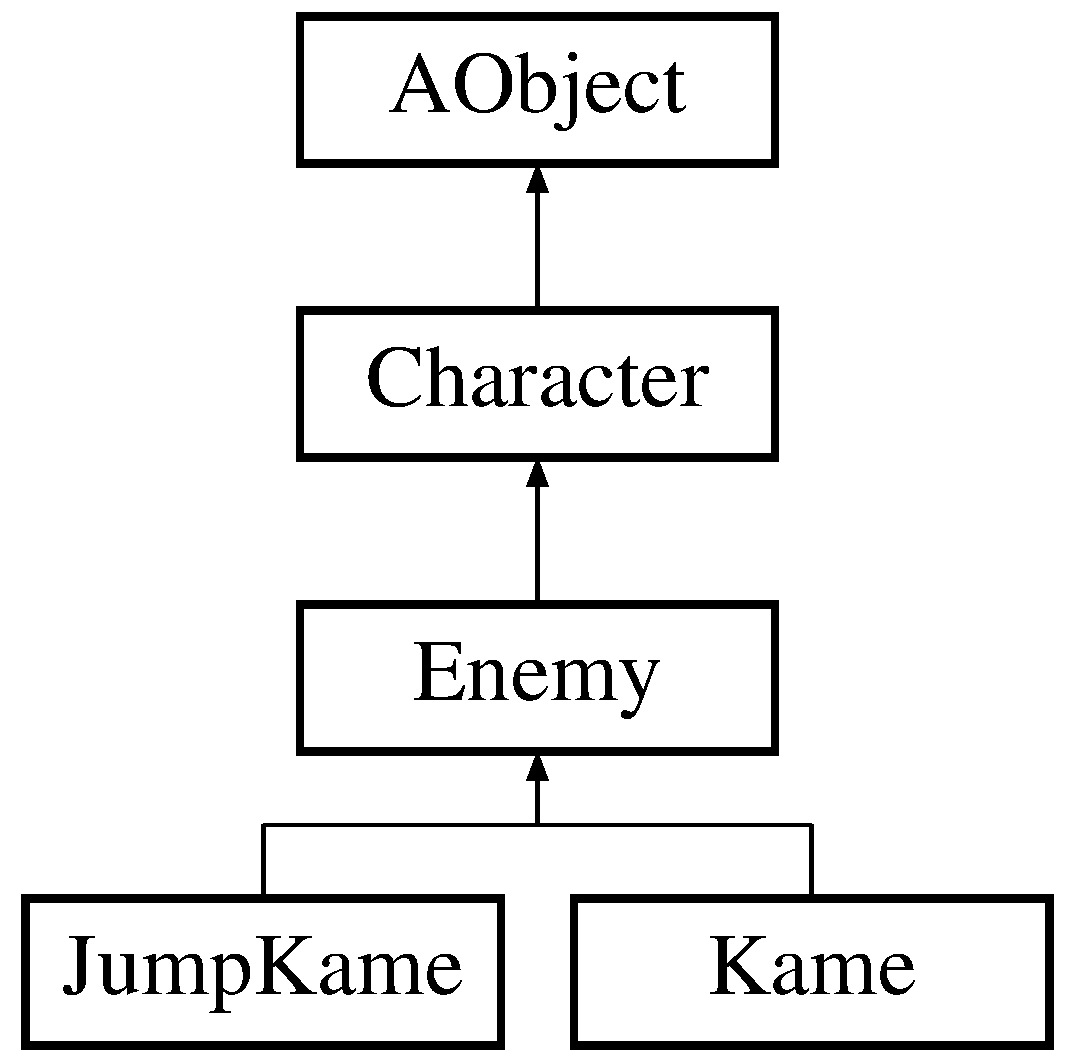
\includegraphics[height=4.000000cm]{class_enemy}
\end{center}
\end{figure}
\subsection*{公開メンバ関数}
\begin{DoxyCompactItemize}
\item 
\hyperlink{class_enemy_a2ac9306a63db9318e5508176f4d0e21a}{Enemy} (double x, double y, int \hyperlink{class_character_a7ea1356e63b9c74e9568feec5e1c92f5}{hp}, char $\ast$file\+\_\+name, int size\+\_\+x, int size\+\_\+y, \hyperlink{class_character_controller}{Character\+Controller} $\ast$controller, \hyperlink{class_attack}{Attack} $\ast$attakck)
\end{DoxyCompactItemize}
\subsection*{その他の継承メンバ}


\subsection{構築子と解体子}
\hypertarget{class_enemy_a2ac9306a63db9318e5508176f4d0e21a}{\index{Enemy@{Enemy}!Enemy@{Enemy}}
\index{Enemy@{Enemy}!Enemy@{Enemy}}
\subsubsection[{Enemy}]{\setlength{\rightskip}{0pt plus 5cm}Enemy\+::\+Enemy (
\begin{DoxyParamCaption}
\item[{double}]{x, }
\item[{double}]{y, }
\item[{int}]{hp, }
\item[{char $\ast$}]{file\+\_\+name, }
\item[{int}]{size\+\_\+x, }
\item[{int}]{size\+\_\+y, }
\item[{{\bf Character\+Controller} $\ast$}]{controller, }
\item[{{\bf Attack} $\ast$}]{attakck}
\end{DoxyParamCaption}
)}}\label{class_enemy_a2ac9306a63db9318e5508176f4d0e21a}


このクラス詳解は次のファイルから抽出されました\+:\begin{DoxyCompactItemize}
\item 
\hyperlink{_enemy_8h}{Enemy.\+h}\item 
\hyperlink{_enemy_8cpp}{Enemy.\+cpp}\end{DoxyCompactItemize}

\hypertarget{class_field}{\section{Field クラス}
\label{class_field}\index{Field@{Field}}
}


{\ttfamily \#include $<$Field.\+h$>$}

\subsection*{公開メンバ関数}
\begin{DoxyCompactItemize}
\item 
\hyperlink{class_field_a3e804c92273d9159f413f227b535c672}{Field} ()
\item 
\hyperlink{class_field_ac3b19f4f5451b19638479e4e6302a465}{Field} (\hyperlink{class_map}{Map} $\ast$map)
\item 
int \hyperlink{class_field_abe0201576e9a90b0c971d0531a834fe0}{Main\+Loop} ()
\item 
int \hyperlink{class_field_aef2ba50ec80860898b18cc14f76821bb}{Get\+Map\+Data} (double x, double y)
\item 
int \hyperlink{class_field_a42b76e7d36c36525c8f23da05f5ef451}{Get\+Next\+Map\+Data} (\hyperlink{struct_two_dimension}{Two\+Dimension} chara\+\_\+pos, \hyperlink{struct_two_dimension}{Two\+Dimension} chara\+\_\+speed, bool right)
\item 
\hyperlink{struct_two_dimension}{Two\+Dimension} \hyperlink{class_field_a701edaa0540555c8087df537402e5e22}{Get\+Player\+Pos} ()
\item 
int \hyperlink{class_field_a7fd8d8172b36ef5f764e9b98b178c8eb}{count} ()
\item 
\hyperlink{class_player}{Player} $\ast$ \hyperlink{class_field_aa135a6f54b5b6779b36e147e46c70696}{player} ()
\item 
\hyperlink{class_field_a45d6e6d09b8f8e46de62b40119d62c60}{$\sim$\+Field} ()
\end{DoxyCompactItemize}
\subsection*{非公開メンバ関数}
\begin{DoxyCompactItemize}
\item 
void \hyperlink{class_field_a1eda9df5b8cb72839ed042921025fb65}{Initialize} ()
\item 
void \hyperlink{class_field_a433cb83e730fd4ed4c773fb3eb32919c}{Scroll} ()
\item 
void \hyperlink{class_field_aab548ccb15ba5e71cd81880a40fcb1c2}{Fall\+Objects} ()
\item 
void \hyperlink{class_field_a5b46210e4fa643128ce37b654f5eea90}{Move\+Objects} ()
\item 
void \hyperlink{class_field_a1addadd366450a3d89a09213b354cbde}{Draw\+Objects} ()
\item 
void \hyperlink{class_field_a9fdfb39458b7f28b0084ff4f0ba306ab}{Think\+Objects} ()
\item 
void \hyperlink{class_field_a527bab59bc982d71e31d08a8f19012a2}{Touch\+Player\+To\+Objects} ()
\item 
void \hyperlink{class_field_a9e2f9ec9dea92779d4ad10ef5317c9bd}{Touch\+Objects\+To\+Wall} ()
\item 
void \hyperlink{class_field_a68718c2c362cb7586112993c765306af}{Bullet\+Touch\+Wall} ()
\item 
void \hyperlink{class_field_aa0d2a42df398cb284aded394edd765ca}{Reset} ()
\item 
void \hyperlink{class_field_a95aed395fb1b9c1d771adb49147387a3}{Game\+Over} ()
\item 
void \hyperlink{class_field_aff3490dddeee21254efb211a535d9c78}{Game\+Clear} ()
\item 
void \hyperlink{class_field_aa099cc4ccf2b6e467484b98cf1d56cb6}{Check\+Out\+Of\+Area} ()
\item 
void \hyperlink{class_field_a3d208f24dd94f42d9ed7a4e63bf34a3c}{Down\+Objects\+Die} ()
\item 
void \hyperlink{class_field_a4a204b53b4884c14eafae7ce359155ce}{Add\+Object} (\hyperlink{class_a_object}{A\+Object} $\ast$object\+\_\+num, bool is\+Begin)
\item 
int \hyperlink{class_field_a36e491f48f9b23b6a165d264babdb2fd}{Pixel\+To\+Tiles} (double pixels)
\item 
int \hyperlink{class_field_ab2167aa053c1d17f8dcfecb47c9acdd2}{Tiles\+To\+Pixels} (int tiles)
\item 
bool \hyperlink{class_field_ab073fa1f34ae99052a1525fb63299b3d}{Judge\+Circle} (int x1, int y1, int r1, int x2, int y2, int r2)
\item 
bool \hyperlink{class_field_a6b4cbd035716adc939657108e0575186}{Judge\+Hit\+Characters} (\hyperlink{class_a_object}{A\+Object} $\ast$p, \hyperlink{class_a_object}{A\+Object} $\ast$e)
\item 
void \hyperlink{class_field_a60fc25acdab8f888ee7791c6f32318ab}{Find\+Object} (int from\+\_\+y, int to\+\_\+y, int from\+\_\+x, int to\+\_\+x)
\end{DoxyCompactItemize}
\subsection*{非公開変数類}
\begin{DoxyCompactItemize}
\item 
\hyperlink{class_map}{Map} $\ast$ \hyperlink{class_field_afa58380f2c246abfac40e368e9a157f0}{map\+\_\+}
\item 
\hyperlink{class_object_manager}{Object\+Manager} $\ast$ \hyperlink{class_field_af51776b9b909f421068a8bcd9701e142}{obj\+\_\+manager\+\_\+}
\item 
int \hyperlink{class_field_a5c4f6af48254c9dcc602879aaf86d03e}{count\+\_\+}
\item 
vector$<$ \hyperlink{class_a_object}{A\+Object} $\ast$ $>$ \hyperlink{class_field_a0e7ed8b2be66267ec1570648f6cdbe40}{objects\+\_\+}
\item 
\hyperlink{class_player}{Player} $\ast$ \hyperlink{class_field_a4376e5c7cac9ae060281c65a9bb10546}{player\+\_\+}
\item 
double \hyperlink{class_field_a3bbc1c73deeb5dc6b2ac78487b121353}{gravity\+\_\+}
\item 
int \hyperlink{class_field_ae160817fea72d1483d556eba3f97dfe6}{offset\+\_\+}
\item 
bool \hyperlink{class_field_a7b31ee36e5115d099c6b7beb47397621}{menu\+\_\+flag}
\item 
int \hyperlink{class_field_a20e399af0fc61f66c5b0a7aadcb5e10b}{wait\+\_\+count\+\_\+}
\item 
int \hyperlink{class_field_ac77b13cecde2f70c728d9a8d4355928e}{end\+\_\+graphic\+\_\+handle}
\item 
int \hyperlink{class_field_a00ee4da146cd30fce7aa9e7ce5b3a781}{clear\+\_\+graphic\+\_\+handle}
\end{DoxyCompactItemize}


\subsection{構築子と解体子}
\hypertarget{class_field_a3e804c92273d9159f413f227b535c672}{\index{Field@{Field}!Field@{Field}}
\index{Field@{Field}!Field@{Field}}
\subsubsection[{Field}]{\setlength{\rightskip}{0pt plus 5cm}Field\+::\+Field (
\begin{DoxyParamCaption}
{}
\end{DoxyParamCaption}
)}}\label{class_field_a3e804c92273d9159f413f227b535c672}
\hypertarget{class_field_ac3b19f4f5451b19638479e4e6302a465}{\index{Field@{Field}!Field@{Field}}
\index{Field@{Field}!Field@{Field}}
\subsubsection[{Field}]{\setlength{\rightskip}{0pt plus 5cm}Field\+::\+Field (
\begin{DoxyParamCaption}
\item[{{\bf Map} $\ast$}]{map}
\end{DoxyParamCaption}
)}}\label{class_field_ac3b19f4f5451b19638479e4e6302a465}
\hypertarget{class_field_a45d6e6d09b8f8e46de62b40119d62c60}{\index{Field@{Field}!````~Field@{$\sim$\+Field}}
\index{````~Field@{$\sim$\+Field}!Field@{Field}}
\subsubsection[{$\sim$\+Field}]{\setlength{\rightskip}{0pt plus 5cm}Field\+::$\sim$\+Field (
\begin{DoxyParamCaption}
{}
\end{DoxyParamCaption}
)}}\label{class_field_a45d6e6d09b8f8e46de62b40119d62c60}


\subsection{関数詳解}
\hypertarget{class_field_a4a204b53b4884c14eafae7ce359155ce}{\index{Field@{Field}!Add\+Object@{Add\+Object}}
\index{Add\+Object@{Add\+Object}!Field@{Field}}
\subsubsection[{Add\+Object}]{\setlength{\rightskip}{0pt plus 5cm}void Field\+::\+Add\+Object (
\begin{DoxyParamCaption}
\item[{{\bf A\+Object} $\ast$}]{object\+\_\+num, }
\item[{bool}]{is\+Begin}
\end{DoxyParamCaption}
)\hspace{0.3cm}{\ttfamily [private]}}}\label{class_field_a4a204b53b4884c14eafae7ce359155ce}
\hypertarget{class_field_a68718c2c362cb7586112993c765306af}{\index{Field@{Field}!Bullet\+Touch\+Wall@{Bullet\+Touch\+Wall}}
\index{Bullet\+Touch\+Wall@{Bullet\+Touch\+Wall}!Field@{Field}}
\subsubsection[{Bullet\+Touch\+Wall}]{\setlength{\rightskip}{0pt plus 5cm}void Field\+::\+Bullet\+Touch\+Wall (
\begin{DoxyParamCaption}
{}
\end{DoxyParamCaption}
)\hspace{0.3cm}{\ttfamily [private]}}}\label{class_field_a68718c2c362cb7586112993c765306af}
\hypertarget{class_field_aa099cc4ccf2b6e467484b98cf1d56cb6}{\index{Field@{Field}!Check\+Out\+Of\+Area@{Check\+Out\+Of\+Area}}
\index{Check\+Out\+Of\+Area@{Check\+Out\+Of\+Area}!Field@{Field}}
\subsubsection[{Check\+Out\+Of\+Area}]{\setlength{\rightskip}{0pt plus 5cm}void Field\+::\+Check\+Out\+Of\+Area (
\begin{DoxyParamCaption}
{}
\end{DoxyParamCaption}
)\hspace{0.3cm}{\ttfamily [private]}}}\label{class_field_aa099cc4ccf2b6e467484b98cf1d56cb6}
\hypertarget{class_field_a7fd8d8172b36ef5f764e9b98b178c8eb}{\index{Field@{Field}!count@{count}}
\index{count@{count}!Field@{Field}}
\subsubsection[{count}]{\setlength{\rightskip}{0pt plus 5cm}int Field\+::count (
\begin{DoxyParamCaption}
{}
\end{DoxyParamCaption}
)\hspace{0.3cm}{\ttfamily [inline]}}}\label{class_field_a7fd8d8172b36ef5f764e9b98b178c8eb}
\hypertarget{class_field_a3d208f24dd94f42d9ed7a4e63bf34a3c}{\index{Field@{Field}!Down\+Objects\+Die@{Down\+Objects\+Die}}
\index{Down\+Objects\+Die@{Down\+Objects\+Die}!Field@{Field}}
\subsubsection[{Down\+Objects\+Die}]{\setlength{\rightskip}{0pt plus 5cm}void Field\+::\+Down\+Objects\+Die (
\begin{DoxyParamCaption}
{}
\end{DoxyParamCaption}
)\hspace{0.3cm}{\ttfamily [private]}}}\label{class_field_a3d208f24dd94f42d9ed7a4e63bf34a3c}
\hypertarget{class_field_a1addadd366450a3d89a09213b354cbde}{\index{Field@{Field}!Draw\+Objects@{Draw\+Objects}}
\index{Draw\+Objects@{Draw\+Objects}!Field@{Field}}
\subsubsection[{Draw\+Objects}]{\setlength{\rightskip}{0pt plus 5cm}void Field\+::\+Draw\+Objects (
\begin{DoxyParamCaption}
{}
\end{DoxyParamCaption}
)\hspace{0.3cm}{\ttfamily [private]}}}\label{class_field_a1addadd366450a3d89a09213b354cbde}
\hypertarget{class_field_aab548ccb15ba5e71cd81880a40fcb1c2}{\index{Field@{Field}!Fall\+Objects@{Fall\+Objects}}
\index{Fall\+Objects@{Fall\+Objects}!Field@{Field}}
\subsubsection[{Fall\+Objects}]{\setlength{\rightskip}{0pt plus 5cm}void Field\+::\+Fall\+Objects (
\begin{DoxyParamCaption}
{}
\end{DoxyParamCaption}
)\hspace{0.3cm}{\ttfamily [private]}}}\label{class_field_aab548ccb15ba5e71cd81880a40fcb1c2}
\hypertarget{class_field_a60fc25acdab8f888ee7791c6f32318ab}{\index{Field@{Field}!Find\+Object@{Find\+Object}}
\index{Find\+Object@{Find\+Object}!Field@{Field}}
\subsubsection[{Find\+Object}]{\setlength{\rightskip}{0pt plus 5cm}void Field\+::\+Find\+Object (
\begin{DoxyParamCaption}
\item[{int}]{from\+\_\+y, }
\item[{int}]{to\+\_\+y, }
\item[{int}]{from\+\_\+x, }
\item[{int}]{to\+\_\+x}
\end{DoxyParamCaption}
)\hspace{0.3cm}{\ttfamily [private]}}}\label{class_field_a60fc25acdab8f888ee7791c6f32318ab}
\hypertarget{class_field_aff3490dddeee21254efb211a535d9c78}{\index{Field@{Field}!Game\+Clear@{Game\+Clear}}
\index{Game\+Clear@{Game\+Clear}!Field@{Field}}
\subsubsection[{Game\+Clear}]{\setlength{\rightskip}{0pt plus 5cm}void Field\+::\+Game\+Clear (
\begin{DoxyParamCaption}
{}
\end{DoxyParamCaption}
)\hspace{0.3cm}{\ttfamily [private]}}}\label{class_field_aff3490dddeee21254efb211a535d9c78}
\hypertarget{class_field_a95aed395fb1b9c1d771adb49147387a3}{\index{Field@{Field}!Game\+Over@{Game\+Over}}
\index{Game\+Over@{Game\+Over}!Field@{Field}}
\subsubsection[{Game\+Over}]{\setlength{\rightskip}{0pt plus 5cm}void Field\+::\+Game\+Over (
\begin{DoxyParamCaption}
{}
\end{DoxyParamCaption}
)\hspace{0.3cm}{\ttfamily [private]}}}\label{class_field_a95aed395fb1b9c1d771adb49147387a3}
\hypertarget{class_field_aef2ba50ec80860898b18cc14f76821bb}{\index{Field@{Field}!Get\+Map\+Data@{Get\+Map\+Data}}
\index{Get\+Map\+Data@{Get\+Map\+Data}!Field@{Field}}
\subsubsection[{Get\+Map\+Data}]{\setlength{\rightskip}{0pt plus 5cm}int Field\+::\+Get\+Map\+Data (
\begin{DoxyParamCaption}
\item[{double}]{x, }
\item[{double}]{y}
\end{DoxyParamCaption}
)}}\label{class_field_aef2ba50ec80860898b18cc14f76821bb}
\hypertarget{class_field_a42b76e7d36c36525c8f23da05f5ef451}{\index{Field@{Field}!Get\+Next\+Map\+Data@{Get\+Next\+Map\+Data}}
\index{Get\+Next\+Map\+Data@{Get\+Next\+Map\+Data}!Field@{Field}}
\subsubsection[{Get\+Next\+Map\+Data}]{\setlength{\rightskip}{0pt plus 5cm}int Field\+::\+Get\+Next\+Map\+Data (
\begin{DoxyParamCaption}
\item[{{\bf Two\+Dimension}}]{chara\+\_\+pos, }
\item[{{\bf Two\+Dimension}}]{chara\+\_\+speed, }
\item[{bool}]{right}
\end{DoxyParamCaption}
)}}\label{class_field_a42b76e7d36c36525c8f23da05f5ef451}
\hypertarget{class_field_a701edaa0540555c8087df537402e5e22}{\index{Field@{Field}!Get\+Player\+Pos@{Get\+Player\+Pos}}
\index{Get\+Player\+Pos@{Get\+Player\+Pos}!Field@{Field}}
\subsubsection[{Get\+Player\+Pos}]{\setlength{\rightskip}{0pt plus 5cm}{\bf Two\+Dimension} Field\+::\+Get\+Player\+Pos (
\begin{DoxyParamCaption}
{}
\end{DoxyParamCaption}
)}}\label{class_field_a701edaa0540555c8087df537402e5e22}
\hypertarget{class_field_a1eda9df5b8cb72839ed042921025fb65}{\index{Field@{Field}!Initialize@{Initialize}}
\index{Initialize@{Initialize}!Field@{Field}}
\subsubsection[{Initialize}]{\setlength{\rightskip}{0pt plus 5cm}void Field\+::\+Initialize (
\begin{DoxyParamCaption}
{}
\end{DoxyParamCaption}
)\hspace{0.3cm}{\ttfamily [private]}}}\label{class_field_a1eda9df5b8cb72839ed042921025fb65}
\hypertarget{class_field_ab073fa1f34ae99052a1525fb63299b3d}{\index{Field@{Field}!Judge\+Circle@{Judge\+Circle}}
\index{Judge\+Circle@{Judge\+Circle}!Field@{Field}}
\subsubsection[{Judge\+Circle}]{\setlength{\rightskip}{0pt plus 5cm}bool Field\+::\+Judge\+Circle (
\begin{DoxyParamCaption}
\item[{int}]{x1, }
\item[{int}]{y1, }
\item[{int}]{r1, }
\item[{int}]{x2, }
\item[{int}]{y2, }
\item[{int}]{r2}
\end{DoxyParamCaption}
)\hspace{0.3cm}{\ttfamily [private]}}}\label{class_field_ab073fa1f34ae99052a1525fb63299b3d}
\hypertarget{class_field_a6b4cbd035716adc939657108e0575186}{\index{Field@{Field}!Judge\+Hit\+Characters@{Judge\+Hit\+Characters}}
\index{Judge\+Hit\+Characters@{Judge\+Hit\+Characters}!Field@{Field}}
\subsubsection[{Judge\+Hit\+Characters}]{\setlength{\rightskip}{0pt plus 5cm}bool Field\+::\+Judge\+Hit\+Characters (
\begin{DoxyParamCaption}
\item[{{\bf A\+Object} $\ast$}]{p, }
\item[{{\bf A\+Object} $\ast$}]{e}
\end{DoxyParamCaption}
)\hspace{0.3cm}{\ttfamily [private]}}}\label{class_field_a6b4cbd035716adc939657108e0575186}
\hypertarget{class_field_abe0201576e9a90b0c971d0531a834fe0}{\index{Field@{Field}!Main\+Loop@{Main\+Loop}}
\index{Main\+Loop@{Main\+Loop}!Field@{Field}}
\subsubsection[{Main\+Loop}]{\setlength{\rightskip}{0pt plus 5cm}int Field\+::\+Main\+Loop (
\begin{DoxyParamCaption}
{}
\end{DoxyParamCaption}
)}}\label{class_field_abe0201576e9a90b0c971d0531a834fe0}
\hypertarget{class_field_a5b46210e4fa643128ce37b654f5eea90}{\index{Field@{Field}!Move\+Objects@{Move\+Objects}}
\index{Move\+Objects@{Move\+Objects}!Field@{Field}}
\subsubsection[{Move\+Objects}]{\setlength{\rightskip}{0pt plus 5cm}void Field\+::\+Move\+Objects (
\begin{DoxyParamCaption}
{}
\end{DoxyParamCaption}
)\hspace{0.3cm}{\ttfamily [private]}}}\label{class_field_a5b46210e4fa643128ce37b654f5eea90}
\hypertarget{class_field_a36e491f48f9b23b6a165d264babdb2fd}{\index{Field@{Field}!Pixel\+To\+Tiles@{Pixel\+To\+Tiles}}
\index{Pixel\+To\+Tiles@{Pixel\+To\+Tiles}!Field@{Field}}
\subsubsection[{Pixel\+To\+Tiles}]{\setlength{\rightskip}{0pt plus 5cm}int Field\+::\+Pixel\+To\+Tiles (
\begin{DoxyParamCaption}
\item[{double}]{pixels}
\end{DoxyParamCaption}
)\hspace{0.3cm}{\ttfamily [private]}}}\label{class_field_a36e491f48f9b23b6a165d264babdb2fd}
\hypertarget{class_field_aa135a6f54b5b6779b36e147e46c70696}{\index{Field@{Field}!player@{player}}
\index{player@{player}!Field@{Field}}
\subsubsection[{player}]{\setlength{\rightskip}{0pt plus 5cm}{\bf Player}$\ast$ Field\+::player (
\begin{DoxyParamCaption}
{}
\end{DoxyParamCaption}
)\hspace{0.3cm}{\ttfamily [inline]}}}\label{class_field_aa135a6f54b5b6779b36e147e46c70696}
\hypertarget{class_field_aa0d2a42df398cb284aded394edd765ca}{\index{Field@{Field}!Reset@{Reset}}
\index{Reset@{Reset}!Field@{Field}}
\subsubsection[{Reset}]{\setlength{\rightskip}{0pt plus 5cm}void Field\+::\+Reset (
\begin{DoxyParamCaption}
{}
\end{DoxyParamCaption}
)\hspace{0.3cm}{\ttfamily [private]}}}\label{class_field_aa0d2a42df398cb284aded394edd765ca}
\hypertarget{class_field_a433cb83e730fd4ed4c773fb3eb32919c}{\index{Field@{Field}!Scroll@{Scroll}}
\index{Scroll@{Scroll}!Field@{Field}}
\subsubsection[{Scroll}]{\setlength{\rightskip}{0pt plus 5cm}void Field\+::\+Scroll (
\begin{DoxyParamCaption}
{}
\end{DoxyParamCaption}
)\hspace{0.3cm}{\ttfamily [private]}}}\label{class_field_a433cb83e730fd4ed4c773fb3eb32919c}
\hypertarget{class_field_a9fdfb39458b7f28b0084ff4f0ba306ab}{\index{Field@{Field}!Think\+Objects@{Think\+Objects}}
\index{Think\+Objects@{Think\+Objects}!Field@{Field}}
\subsubsection[{Think\+Objects}]{\setlength{\rightskip}{0pt plus 5cm}void Field\+::\+Think\+Objects (
\begin{DoxyParamCaption}
{}
\end{DoxyParamCaption}
)\hspace{0.3cm}{\ttfamily [private]}}}\label{class_field_a9fdfb39458b7f28b0084ff4f0ba306ab}
\hypertarget{class_field_ab2167aa053c1d17f8dcfecb47c9acdd2}{\index{Field@{Field}!Tiles\+To\+Pixels@{Tiles\+To\+Pixels}}
\index{Tiles\+To\+Pixels@{Tiles\+To\+Pixels}!Field@{Field}}
\subsubsection[{Tiles\+To\+Pixels}]{\setlength{\rightskip}{0pt plus 5cm}int Field\+::\+Tiles\+To\+Pixels (
\begin{DoxyParamCaption}
\item[{int}]{tiles}
\end{DoxyParamCaption}
)\hspace{0.3cm}{\ttfamily [private]}}}\label{class_field_ab2167aa053c1d17f8dcfecb47c9acdd2}
\hypertarget{class_field_a9e2f9ec9dea92779d4ad10ef5317c9bd}{\index{Field@{Field}!Touch\+Objects\+To\+Wall@{Touch\+Objects\+To\+Wall}}
\index{Touch\+Objects\+To\+Wall@{Touch\+Objects\+To\+Wall}!Field@{Field}}
\subsubsection[{Touch\+Objects\+To\+Wall}]{\setlength{\rightskip}{0pt plus 5cm}void Field\+::\+Touch\+Objects\+To\+Wall (
\begin{DoxyParamCaption}
{}
\end{DoxyParamCaption}
)\hspace{0.3cm}{\ttfamily [private]}}}\label{class_field_a9e2f9ec9dea92779d4ad10ef5317c9bd}
\hypertarget{class_field_a527bab59bc982d71e31d08a8f19012a2}{\index{Field@{Field}!Touch\+Player\+To\+Objects@{Touch\+Player\+To\+Objects}}
\index{Touch\+Player\+To\+Objects@{Touch\+Player\+To\+Objects}!Field@{Field}}
\subsubsection[{Touch\+Player\+To\+Objects}]{\setlength{\rightskip}{0pt plus 5cm}void Field\+::\+Touch\+Player\+To\+Objects (
\begin{DoxyParamCaption}
{}
\end{DoxyParamCaption}
)\hspace{0.3cm}{\ttfamily [private]}}}\label{class_field_a527bab59bc982d71e31d08a8f19012a2}


\subsection{メンバ詳解}
\hypertarget{class_field_a00ee4da146cd30fce7aa9e7ce5b3a781}{\index{Field@{Field}!clear\+\_\+graphic\+\_\+handle@{clear\+\_\+graphic\+\_\+handle}}
\index{clear\+\_\+graphic\+\_\+handle@{clear\+\_\+graphic\+\_\+handle}!Field@{Field}}
\subsubsection[{clear\+\_\+graphic\+\_\+handle}]{\setlength{\rightskip}{0pt plus 5cm}int Field\+::clear\+\_\+graphic\+\_\+handle\hspace{0.3cm}{\ttfamily [private]}}}\label{class_field_a00ee4da146cd30fce7aa9e7ce5b3a781}
\hypertarget{class_field_a5c4f6af48254c9dcc602879aaf86d03e}{\index{Field@{Field}!count\+\_\+@{count\+\_\+}}
\index{count\+\_\+@{count\+\_\+}!Field@{Field}}
\subsubsection[{count\+\_\+}]{\setlength{\rightskip}{0pt plus 5cm}int Field\+::count\+\_\+\hspace{0.3cm}{\ttfamily [private]}}}\label{class_field_a5c4f6af48254c9dcc602879aaf86d03e}
\hypertarget{class_field_ac77b13cecde2f70c728d9a8d4355928e}{\index{Field@{Field}!end\+\_\+graphic\+\_\+handle@{end\+\_\+graphic\+\_\+handle}}
\index{end\+\_\+graphic\+\_\+handle@{end\+\_\+graphic\+\_\+handle}!Field@{Field}}
\subsubsection[{end\+\_\+graphic\+\_\+handle}]{\setlength{\rightskip}{0pt plus 5cm}int Field\+::end\+\_\+graphic\+\_\+handle\hspace{0.3cm}{\ttfamily [private]}}}\label{class_field_ac77b13cecde2f70c728d9a8d4355928e}
\hypertarget{class_field_a3bbc1c73deeb5dc6b2ac78487b121353}{\index{Field@{Field}!gravity\+\_\+@{gravity\+\_\+}}
\index{gravity\+\_\+@{gravity\+\_\+}!Field@{Field}}
\subsubsection[{gravity\+\_\+}]{\setlength{\rightskip}{0pt plus 5cm}double Field\+::gravity\+\_\+\hspace{0.3cm}{\ttfamily [private]}}}\label{class_field_a3bbc1c73deeb5dc6b2ac78487b121353}
\hypertarget{class_field_afa58380f2c246abfac40e368e9a157f0}{\index{Field@{Field}!map\+\_\+@{map\+\_\+}}
\index{map\+\_\+@{map\+\_\+}!Field@{Field}}
\subsubsection[{map\+\_\+}]{\setlength{\rightskip}{0pt plus 5cm}{\bf Map}$\ast$ Field\+::map\+\_\+\hspace{0.3cm}{\ttfamily [private]}}}\label{class_field_afa58380f2c246abfac40e368e9a157f0}
\hypertarget{class_field_a7b31ee36e5115d099c6b7beb47397621}{\index{Field@{Field}!menu\+\_\+flag@{menu\+\_\+flag}}
\index{menu\+\_\+flag@{menu\+\_\+flag}!Field@{Field}}
\subsubsection[{menu\+\_\+flag}]{\setlength{\rightskip}{0pt plus 5cm}bool Field\+::menu\+\_\+flag\hspace{0.3cm}{\ttfamily [private]}}}\label{class_field_a7b31ee36e5115d099c6b7beb47397621}
\hypertarget{class_field_af51776b9b909f421068a8bcd9701e142}{\index{Field@{Field}!obj\+\_\+manager\+\_\+@{obj\+\_\+manager\+\_\+}}
\index{obj\+\_\+manager\+\_\+@{obj\+\_\+manager\+\_\+}!Field@{Field}}
\subsubsection[{obj\+\_\+manager\+\_\+}]{\setlength{\rightskip}{0pt plus 5cm}{\bf Object\+Manager}$\ast$ Field\+::obj\+\_\+manager\+\_\+\hspace{0.3cm}{\ttfamily [private]}}}\label{class_field_af51776b9b909f421068a8bcd9701e142}
\hypertarget{class_field_a0e7ed8b2be66267ec1570648f6cdbe40}{\index{Field@{Field}!objects\+\_\+@{objects\+\_\+}}
\index{objects\+\_\+@{objects\+\_\+}!Field@{Field}}
\subsubsection[{objects\+\_\+}]{\setlength{\rightskip}{0pt plus 5cm}vector$<${\bf A\+Object}$\ast$$>$ Field\+::objects\+\_\+\hspace{0.3cm}{\ttfamily [private]}}}\label{class_field_a0e7ed8b2be66267ec1570648f6cdbe40}
\hypertarget{class_field_ae160817fea72d1483d556eba3f97dfe6}{\index{Field@{Field}!offset\+\_\+@{offset\+\_\+}}
\index{offset\+\_\+@{offset\+\_\+}!Field@{Field}}
\subsubsection[{offset\+\_\+}]{\setlength{\rightskip}{0pt plus 5cm}int Field\+::offset\+\_\+\hspace{0.3cm}{\ttfamily [private]}}}\label{class_field_ae160817fea72d1483d556eba3f97dfe6}
\hypertarget{class_field_a4376e5c7cac9ae060281c65a9bb10546}{\index{Field@{Field}!player\+\_\+@{player\+\_\+}}
\index{player\+\_\+@{player\+\_\+}!Field@{Field}}
\subsubsection[{player\+\_\+}]{\setlength{\rightskip}{0pt plus 5cm}{\bf Player}$\ast$ Field\+::player\+\_\+\hspace{0.3cm}{\ttfamily [private]}}}\label{class_field_a4376e5c7cac9ae060281c65a9bb10546}
\hypertarget{class_field_a20e399af0fc61f66c5b0a7aadcb5e10b}{\index{Field@{Field}!wait\+\_\+count\+\_\+@{wait\+\_\+count\+\_\+}}
\index{wait\+\_\+count\+\_\+@{wait\+\_\+count\+\_\+}!Field@{Field}}
\subsubsection[{wait\+\_\+count\+\_\+}]{\setlength{\rightskip}{0pt plus 5cm}int Field\+::wait\+\_\+count\+\_\+\hspace{0.3cm}{\ttfamily [private]}}}\label{class_field_a20e399af0fc61f66c5b0a7aadcb5e10b}


このクラス詳解は次のファイルから抽出されました\+:\begin{DoxyCompactItemize}
\item 
\hyperlink{_field_8h}{Field.\+h}\item 
\hyperlink{_field_8cpp}{Field.\+cpp}\end{DoxyCompactItemize}

\hypertarget{class_game_main}{\section{Game\+Main クラス}
\label{class_game_main}\index{Game\+Main@{Game\+Main}}
}


{\ttfamily \#include $<$Game\+Main.\+h$>$}

\subsection*{公開メンバ関数}
\begin{DoxyCompactItemize}
\item 
void \hyperlink{class_game_main_a33ec044049ba66a511632776ea609246}{Game\+Start} ()
\item 
void \hyperlink{class_game_main_ad9475bacd59874a961c715f9347eb57e}{Main\+Loop} ()
\item 
\hyperlink{class_game_main_acc3bbdc99511554dd9afda65e7d5f0ef}{Game\+Main} ()
\end{DoxyCompactItemize}
\subsection*{公開変数類}
\begin{DoxyCompactItemize}
\item 
int \hyperlink{class_game_main_a7e8d331a37fb0910a8369e0f971eac72}{m\+Start\+Time}
\item 
int \hyperlink{class_game_main_a75b2b9e2818a643f4ed5ee8a02132516}{m\+Count}
\item 
float \hyperlink{class_game_main_a796aea62906d2d46927a4f12420e9620}{m\+Fps}
\end{DoxyCompactItemize}
\subsection*{静的公開変数類}
\begin{DoxyCompactItemize}
\item 
static const int \hyperlink{class_game_main_af369063b5921fa53f89d3c34ca8ab8c3}{N} = 60
\item 
static const int \hyperlink{class_game_main_a58fcd65ed83d0f30475149e084354040}{F\+P\+S} = 60
\end{DoxyCompactItemize}
\subsection*{非公開メンバ関数}
\begin{DoxyCompactItemize}
\item 
bool \hyperlink{class_game_main_aaa2bf042f2c2615180bb3accc74d4f34}{Update} ()
\item 
void \hyperlink{class_game_main_aecebe55e01987341eb5a934de103894f}{Draw} ()
\item 
void \hyperlink{class_game_main_ad0def9978a87d0becdf781a6bb051096}{Wait} ()
\end{DoxyCompactItemize}
\subsection*{非公開変数類}
\begin{DoxyCompactItemize}
\item 
\hyperlink{class_field}{Field} $\ast$ \hyperlink{class_game_main_a5588fbeddda88c3591ae3fb03d9cdfb4}{field}
\end{DoxyCompactItemize}


\subsection{構築子と解体子}
\hypertarget{class_game_main_acc3bbdc99511554dd9afda65e7d5f0ef}{\index{Game\+Main@{Game\+Main}!Game\+Main@{Game\+Main}}
\index{Game\+Main@{Game\+Main}!Game\+Main@{Game\+Main}}
\subsubsection[{Game\+Main}]{\setlength{\rightskip}{0pt plus 5cm}Game\+Main\+::\+Game\+Main (
\begin{DoxyParamCaption}
{}
\end{DoxyParamCaption}
)}}\label{class_game_main_acc3bbdc99511554dd9afda65e7d5f0ef}


\subsection{関数詳解}
\hypertarget{class_game_main_aecebe55e01987341eb5a934de103894f}{\index{Game\+Main@{Game\+Main}!Draw@{Draw}}
\index{Draw@{Draw}!Game\+Main@{Game\+Main}}
\subsubsection[{Draw}]{\setlength{\rightskip}{0pt plus 5cm}void Game\+Main\+::\+Draw (
\begin{DoxyParamCaption}
{}
\end{DoxyParamCaption}
)\hspace{0.3cm}{\ttfamily [private]}}}\label{class_game_main_aecebe55e01987341eb5a934de103894f}
\hypertarget{class_game_main_a33ec044049ba66a511632776ea609246}{\index{Game\+Main@{Game\+Main}!Game\+Start@{Game\+Start}}
\index{Game\+Start@{Game\+Start}!Game\+Main@{Game\+Main}}
\subsubsection[{Game\+Start}]{\setlength{\rightskip}{0pt plus 5cm}void Game\+Main\+::\+Game\+Start (
\begin{DoxyParamCaption}
{}
\end{DoxyParamCaption}
)}}\label{class_game_main_a33ec044049ba66a511632776ea609246}
\hypertarget{class_game_main_ad9475bacd59874a961c715f9347eb57e}{\index{Game\+Main@{Game\+Main}!Main\+Loop@{Main\+Loop}}
\index{Main\+Loop@{Main\+Loop}!Game\+Main@{Game\+Main}}
\subsubsection[{Main\+Loop}]{\setlength{\rightskip}{0pt plus 5cm}void Game\+Main\+::\+Main\+Loop (
\begin{DoxyParamCaption}
{}
\end{DoxyParamCaption}
)}}\label{class_game_main_ad9475bacd59874a961c715f9347eb57e}
\hypertarget{class_game_main_aaa2bf042f2c2615180bb3accc74d4f34}{\index{Game\+Main@{Game\+Main}!Update@{Update}}
\index{Update@{Update}!Game\+Main@{Game\+Main}}
\subsubsection[{Update}]{\setlength{\rightskip}{0pt plus 5cm}bool Game\+Main\+::\+Update (
\begin{DoxyParamCaption}
{}
\end{DoxyParamCaption}
)\hspace{0.3cm}{\ttfamily [private]}}}\label{class_game_main_aaa2bf042f2c2615180bb3accc74d4f34}
\hypertarget{class_game_main_ad0def9978a87d0becdf781a6bb051096}{\index{Game\+Main@{Game\+Main}!Wait@{Wait}}
\index{Wait@{Wait}!Game\+Main@{Game\+Main}}
\subsubsection[{Wait}]{\setlength{\rightskip}{0pt plus 5cm}void Game\+Main\+::\+Wait (
\begin{DoxyParamCaption}
{}
\end{DoxyParamCaption}
)\hspace{0.3cm}{\ttfamily [private]}}}\label{class_game_main_ad0def9978a87d0becdf781a6bb051096}


\subsection{メンバ詳解}
\hypertarget{class_game_main_a5588fbeddda88c3591ae3fb03d9cdfb4}{\index{Game\+Main@{Game\+Main}!field@{field}}
\index{field@{field}!Game\+Main@{Game\+Main}}
\subsubsection[{field}]{\setlength{\rightskip}{0pt plus 5cm}{\bf Field}$\ast$ Game\+Main\+::field\hspace{0.3cm}{\ttfamily [private]}}}\label{class_game_main_a5588fbeddda88c3591ae3fb03d9cdfb4}
\hypertarget{class_game_main_a58fcd65ed83d0f30475149e084354040}{\index{Game\+Main@{Game\+Main}!F\+P\+S@{F\+P\+S}}
\index{F\+P\+S@{F\+P\+S}!Game\+Main@{Game\+Main}}
\subsubsection[{F\+P\+S}]{\setlength{\rightskip}{0pt plus 5cm}const int Game\+Main\+::\+F\+P\+S = 60\hspace{0.3cm}{\ttfamily [static]}}}\label{class_game_main_a58fcd65ed83d0f30475149e084354040}
\hypertarget{class_game_main_a75b2b9e2818a643f4ed5ee8a02132516}{\index{Game\+Main@{Game\+Main}!m\+Count@{m\+Count}}
\index{m\+Count@{m\+Count}!Game\+Main@{Game\+Main}}
\subsubsection[{m\+Count}]{\setlength{\rightskip}{0pt plus 5cm}int Game\+Main\+::m\+Count}}\label{class_game_main_a75b2b9e2818a643f4ed5ee8a02132516}
\hypertarget{class_game_main_a796aea62906d2d46927a4f12420e9620}{\index{Game\+Main@{Game\+Main}!m\+Fps@{m\+Fps}}
\index{m\+Fps@{m\+Fps}!Game\+Main@{Game\+Main}}
\subsubsection[{m\+Fps}]{\setlength{\rightskip}{0pt plus 5cm}float Game\+Main\+::m\+Fps}}\label{class_game_main_a796aea62906d2d46927a4f12420e9620}
\hypertarget{class_game_main_a7e8d331a37fb0910a8369e0f971eac72}{\index{Game\+Main@{Game\+Main}!m\+Start\+Time@{m\+Start\+Time}}
\index{m\+Start\+Time@{m\+Start\+Time}!Game\+Main@{Game\+Main}}
\subsubsection[{m\+Start\+Time}]{\setlength{\rightskip}{0pt plus 5cm}int Game\+Main\+::m\+Start\+Time}}\label{class_game_main_a7e8d331a37fb0910a8369e0f971eac72}
\hypertarget{class_game_main_af369063b5921fa53f89d3c34ca8ab8c3}{\index{Game\+Main@{Game\+Main}!N@{N}}
\index{N@{N}!Game\+Main@{Game\+Main}}
\subsubsection[{N}]{\setlength{\rightskip}{0pt plus 5cm}const int Game\+Main\+::\+N = 60\hspace{0.3cm}{\ttfamily [static]}}}\label{class_game_main_af369063b5921fa53f89d3c34ca8ab8c3}


このクラス詳解は次のファイルから抽出されました\+:\begin{DoxyCompactItemize}
\item 
\hyperlink{_game_main_8h}{Game\+Main.\+h}\item 
\hyperlink{_game_main_8cpp}{Game\+Main.\+cpp}\end{DoxyCompactItemize}

\hypertarget{class_goal_flag}{\section{Goal\+Flag クラス}
\label{class_goal_flag}\index{Goal\+Flag@{Goal\+Flag}}
}


{\ttfamily \#include $<$Goal\+Flag.\+h$>$}

Goal\+Flag の継承関係図\begin{figure}[H]
\begin{center}
\leavevmode
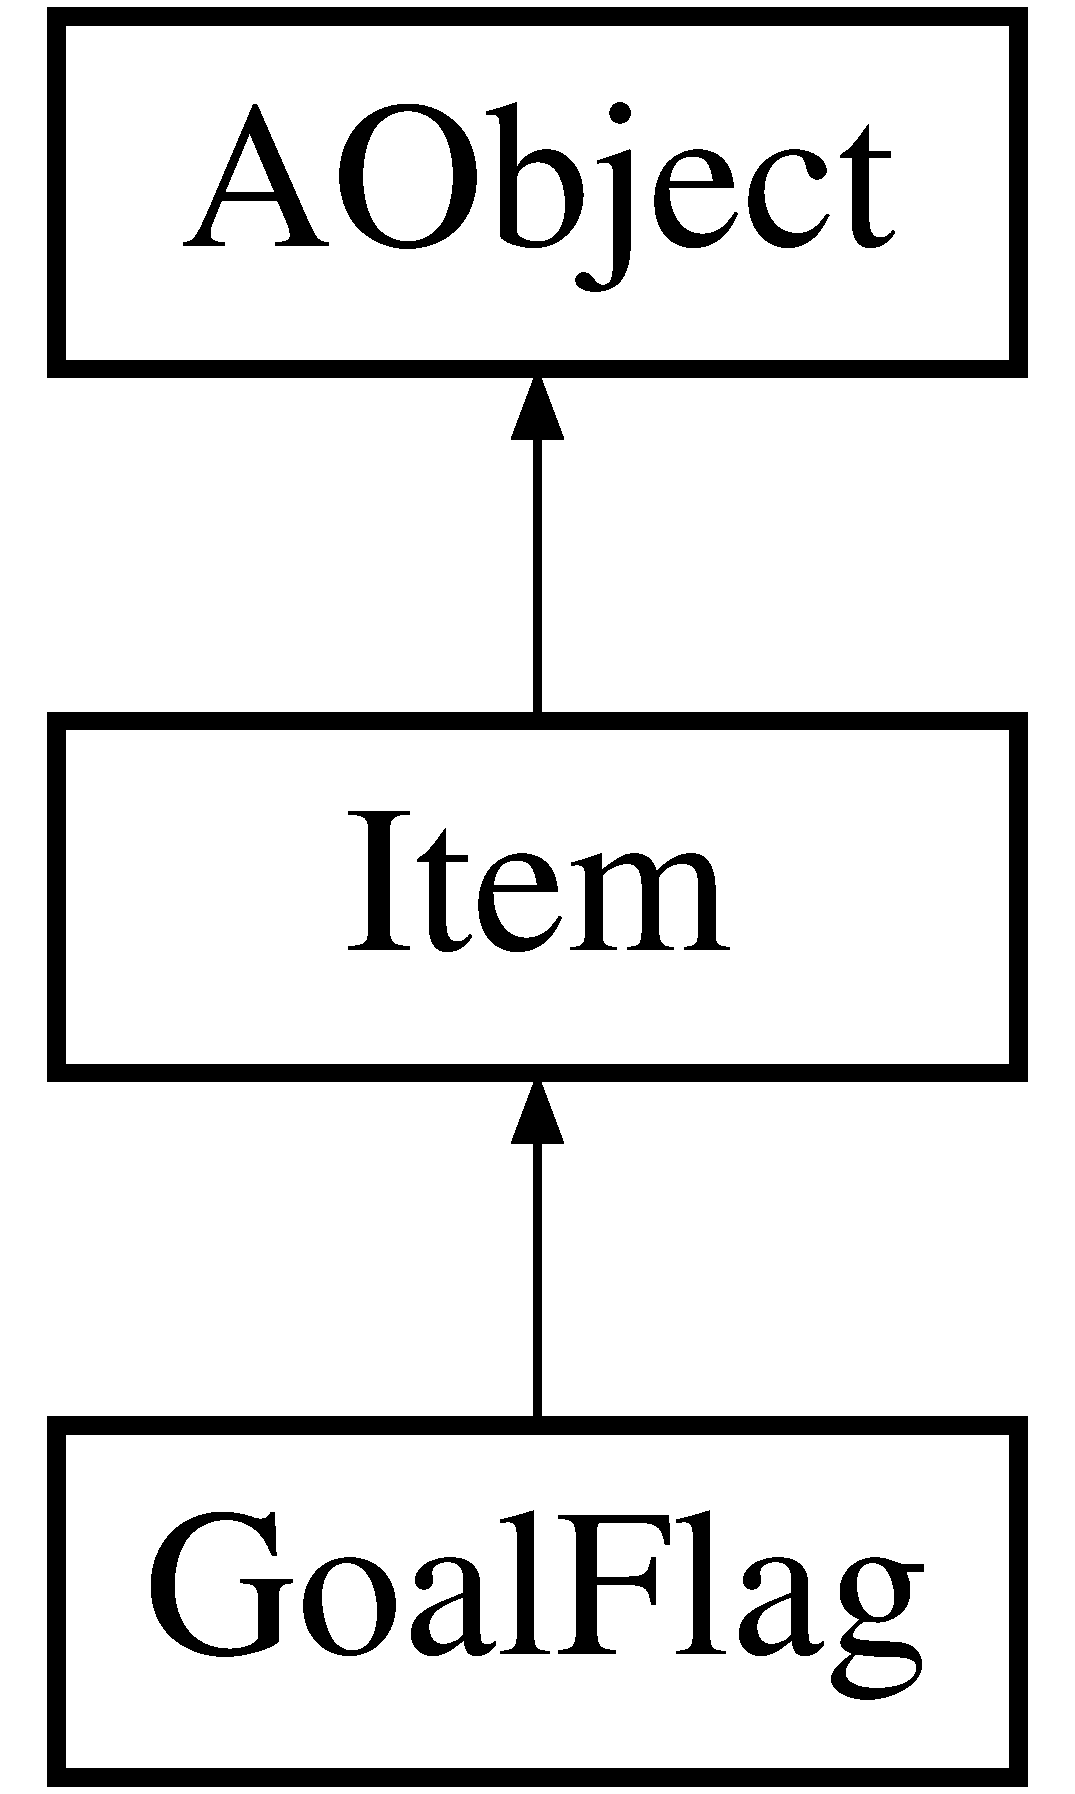
\includegraphics[height=3.000000cm]{class_goal_flag}
\end{center}
\end{figure}
\subsection*{公開メンバ関数}
\begin{DoxyCompactItemize}
\item 
\hyperlink{class_goal_flag_ada22757156d5fafce9133c5f78b768dd}{Goal\+Flag} (double x, double y)
\item 
void \hyperlink{class_goal_flag_a12f6b5e7622fb8ff23381f804ffee2a6}{Affect} (\hyperlink{class_character}{Character} $\ast$character)
\item 
void \hyperlink{class_goal_flag_a343f277b68067d9d19bff4815b14c6ac}{Think} ()
\end{DoxyCompactItemize}
\subsection*{その他の継承メンバ}


\subsection{構築子と解体子}
\hypertarget{class_goal_flag_ada22757156d5fafce9133c5f78b768dd}{\index{Goal\+Flag@{Goal\+Flag}!Goal\+Flag@{Goal\+Flag}}
\index{Goal\+Flag@{Goal\+Flag}!Goal\+Flag@{Goal\+Flag}}
\subsubsection[{Goal\+Flag}]{\setlength{\rightskip}{0pt plus 5cm}Goal\+Flag\+::\+Goal\+Flag (
\begin{DoxyParamCaption}
\item[{double}]{x, }
\item[{double}]{y}
\end{DoxyParamCaption}
)}}\label{class_goal_flag_ada22757156d5fafce9133c5f78b768dd}


\subsection{関数詳解}
\hypertarget{class_goal_flag_a12f6b5e7622fb8ff23381f804ffee2a6}{\index{Goal\+Flag@{Goal\+Flag}!Affect@{Affect}}
\index{Affect@{Affect}!Goal\+Flag@{Goal\+Flag}}
\subsubsection[{Affect}]{\setlength{\rightskip}{0pt plus 5cm}void Goal\+Flag\+::\+Affect (
\begin{DoxyParamCaption}
\item[{{\bf Character} $\ast$}]{character}
\end{DoxyParamCaption}
)\hspace{0.3cm}{\ttfamily [virtual]}}}\label{class_goal_flag_a12f6b5e7622fb8ff23381f804ffee2a6}


\hyperlink{class_item_a3102747c3c78a04691d821d1be363354}{Item}を実装しています。

\hypertarget{class_goal_flag_a343f277b68067d9d19bff4815b14c6ac}{\index{Goal\+Flag@{Goal\+Flag}!Think@{Think}}
\index{Think@{Think}!Goal\+Flag@{Goal\+Flag}}
\subsubsection[{Think}]{\setlength{\rightskip}{0pt plus 5cm}void Goal\+Flag\+::\+Think (
\begin{DoxyParamCaption}
{}
\end{DoxyParamCaption}
)\hspace{0.3cm}{\ttfamily [virtual]}}}\label{class_goal_flag_a343f277b68067d9d19bff4815b14c6ac}


\hyperlink{class_a_object_a61f89197cb14b1270a0a232ee88333a0}{A\+Object}を実装しています。



このクラス詳解は次のファイルから抽出されました\+:\begin{DoxyCompactItemize}
\item 
\hyperlink{_goal_flag_8h}{Goal\+Flag.\+h}\item 
\hyperlink{_goal_flag_8cpp}{Goal\+Flag.\+cpp}\end{DoxyCompactItemize}

\hypertarget{class_item}{\section{Item クラス}
\label{class_item}\index{Item@{Item}}
}


{\ttfamily \#include $<$Item.\+h$>$}

Item の継承関係図\begin{figure}[H]
\begin{center}
\leavevmode
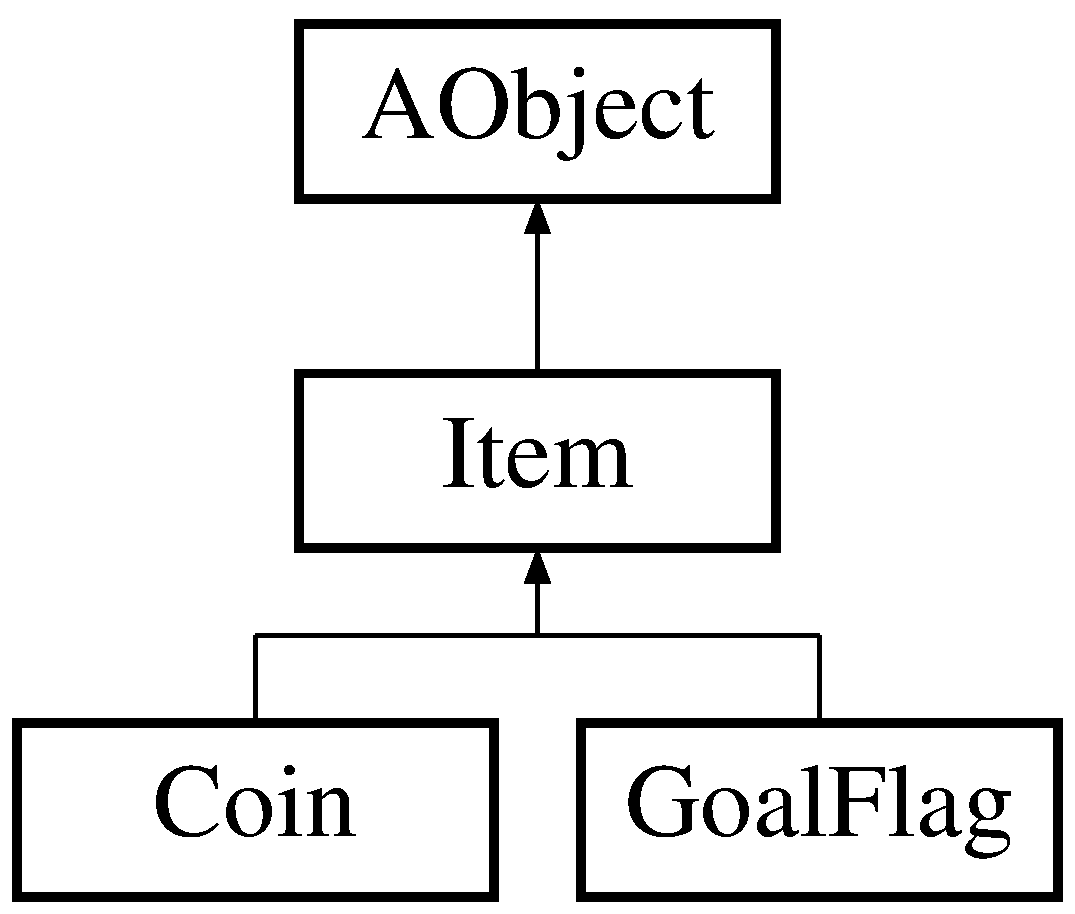
\includegraphics[height=3.000000cm]{class_item}
\end{center}
\end{figure}
\subsection*{公開メンバ関数}
\begin{DoxyCompactItemize}
\item 
\hyperlink{class_item_a49ae437dc08b835517777b3e86c73688}{Item} (double ax, double ay, char $\ast$fname, int size\+\_\+x, int size\+\_\+y, bool \hyperlink{class_a_object_a7453abe76bbddf446aa5787231428a52}{right})
\item 
virtual void \hyperlink{class_item_a3102747c3c78a04691d821d1be363354}{Affect} (\hyperlink{class_character}{Character} $\ast$character)=0
\end{DoxyCompactItemize}
\subsection*{その他の継承メンバ}


\subsection{構築子と解体子}
\hypertarget{class_item_a49ae437dc08b835517777b3e86c73688}{\index{Item@{Item}!Item@{Item}}
\index{Item@{Item}!Item@{Item}}
\subsubsection[{Item}]{\setlength{\rightskip}{0pt plus 5cm}Item\+::\+Item (
\begin{DoxyParamCaption}
\item[{double}]{ax, }
\item[{double}]{ay, }
\item[{char $\ast$}]{fname, }
\item[{int}]{size\+\_\+x, }
\item[{int}]{size\+\_\+y, }
\item[{bool}]{right}
\end{DoxyParamCaption}
)}}\label{class_item_a49ae437dc08b835517777b3e86c73688}


\subsection{関数詳解}
\hypertarget{class_item_a3102747c3c78a04691d821d1be363354}{\index{Item@{Item}!Affect@{Affect}}
\index{Affect@{Affect}!Item@{Item}}
\subsubsection[{Affect}]{\setlength{\rightskip}{0pt plus 5cm}virtual void Item\+::\+Affect (
\begin{DoxyParamCaption}
\item[{{\bf Character} $\ast$}]{character}
\end{DoxyParamCaption}
)\hspace{0.3cm}{\ttfamily [pure virtual]}}}\label{class_item_a3102747c3c78a04691d821d1be363354}


\hyperlink{class_coin_a6991c98735397b008309f713a252d2cd}{Coin}, \hyperlink{class_goal_flag_a12f6b5e7622fb8ff23381f804ffee2a6}{Goal\+Flag}で実装されています。



このクラス詳解は次のファイルから抽出されました\+:\begin{DoxyCompactItemize}
\item 
\hyperlink{_item_8h}{Item.\+h}\item 
\hyperlink{_item_8cpp}{Item.\+cpp}\end{DoxyCompactItemize}

\hypertarget{class_jump_enemy}{\section{Jump\+Enemy クラス}
\label{class_jump_enemy}\index{Jump\+Enemy@{Jump\+Enemy}}
}


{\ttfamily \#include $<$Jump\+Enemy.\+h$>$}

Jump\+Enemy の継承関係図\begin{figure}[H]
\begin{center}
\leavevmode
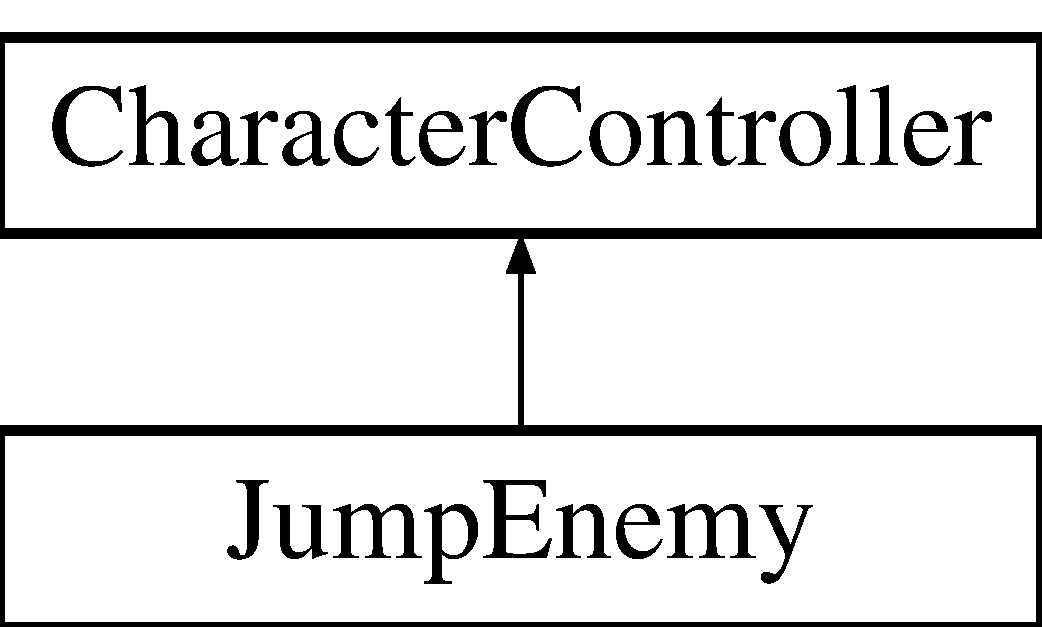
\includegraphics[height=2.000000cm]{class_jump_enemy}
\end{center}
\end{figure}
\subsection*{公開メンバ関数}
\begin{DoxyCompactItemize}
\item 
\hyperlink{class_jump_enemy_a553e827686bca768755f5fb6fe88a425}{Jump\+Enemy} ()
\item 
\hyperlink{class_jump_enemy_ac6a931ac974acd22e7d8a31aa10d1a19}{Jump\+Enemy} (\hyperlink{class_character}{Character} $\ast$character, \hyperlink{class_field}{Field} $\ast$field)
\item 
void \hyperlink{class_jump_enemy_abd7019f8b333e710c1bb65b1b599182c}{Think} ()
\item 
void \hyperlink{class_jump_enemy_a4ab905f21c4526c75a1ae6a436cca601}{Jump} ()
\end{DoxyCompactItemize}
\subsection*{非公開変数類}
\begin{DoxyCompactItemize}
\item 
int \hyperlink{class_jump_enemy_acdb8b9943cefb60493cc8ed9b47d6304}{count}
\end{DoxyCompactItemize}
\subsection*{その他の継承メンバ}


\subsection{構築子と解体子}
\hypertarget{class_jump_enemy_a553e827686bca768755f5fb6fe88a425}{\index{Jump\+Enemy@{Jump\+Enemy}!Jump\+Enemy@{Jump\+Enemy}}
\index{Jump\+Enemy@{Jump\+Enemy}!Jump\+Enemy@{Jump\+Enemy}}
\subsubsection[{Jump\+Enemy}]{\setlength{\rightskip}{0pt plus 5cm}Jump\+Enemy\+::\+Jump\+Enemy (
\begin{DoxyParamCaption}
{}
\end{DoxyParamCaption}
)}}\label{class_jump_enemy_a553e827686bca768755f5fb6fe88a425}
\hypertarget{class_jump_enemy_ac6a931ac974acd22e7d8a31aa10d1a19}{\index{Jump\+Enemy@{Jump\+Enemy}!Jump\+Enemy@{Jump\+Enemy}}
\index{Jump\+Enemy@{Jump\+Enemy}!Jump\+Enemy@{Jump\+Enemy}}
\subsubsection[{Jump\+Enemy}]{\setlength{\rightskip}{0pt plus 5cm}Jump\+Enemy\+::\+Jump\+Enemy (
\begin{DoxyParamCaption}
\item[{{\bf Character} $\ast$}]{character, }
\item[{{\bf Field} $\ast$}]{field}
\end{DoxyParamCaption}
)}}\label{class_jump_enemy_ac6a931ac974acd22e7d8a31aa10d1a19}


\subsection{関数詳解}
\hypertarget{class_jump_enemy_a4ab905f21c4526c75a1ae6a436cca601}{\index{Jump\+Enemy@{Jump\+Enemy}!Jump@{Jump}}
\index{Jump@{Jump}!Jump\+Enemy@{Jump\+Enemy}}
\subsubsection[{Jump}]{\setlength{\rightskip}{0pt plus 5cm}void Jump\+Enemy\+::\+Jump (
\begin{DoxyParamCaption}
{}
\end{DoxyParamCaption}
)}}\label{class_jump_enemy_a4ab905f21c4526c75a1ae6a436cca601}
\hypertarget{class_jump_enemy_abd7019f8b333e710c1bb65b1b599182c}{\index{Jump\+Enemy@{Jump\+Enemy}!Think@{Think}}
\index{Think@{Think}!Jump\+Enemy@{Jump\+Enemy}}
\subsubsection[{Think}]{\setlength{\rightskip}{0pt plus 5cm}void Jump\+Enemy\+::\+Think (
\begin{DoxyParamCaption}
{}
\end{DoxyParamCaption}
)\hspace{0.3cm}{\ttfamily [virtual]}}}\label{class_jump_enemy_abd7019f8b333e710c1bb65b1b599182c}


\hyperlink{class_character_controller_a493d5b59610546133900f4de7110a487}{Character\+Controller}を実装しています。



\subsection{メンバ詳解}
\hypertarget{class_jump_enemy_acdb8b9943cefb60493cc8ed9b47d6304}{\index{Jump\+Enemy@{Jump\+Enemy}!count@{count}}
\index{count@{count}!Jump\+Enemy@{Jump\+Enemy}}
\subsubsection[{count}]{\setlength{\rightskip}{0pt plus 5cm}int Jump\+Enemy\+::count\hspace{0.3cm}{\ttfamily [private]}}}\label{class_jump_enemy_acdb8b9943cefb60493cc8ed9b47d6304}


このクラス詳解は次のファイルから抽出されました\+:\begin{DoxyCompactItemize}
\item 
\hyperlink{_jump_enemy_8h}{Jump\+Enemy.\+h}\item 
\hyperlink{_jump_enemy_8cpp}{Jump\+Enemy.\+cpp}\end{DoxyCompactItemize}

\hypertarget{class_jump_kame}{\section{Jump\+Kame クラス}
\label{class_jump_kame}\index{Jump\+Kame@{Jump\+Kame}}
}


{\ttfamily \#include $<$Jump\+Kame.\+h$>$}

Jump\+Kame の継承関係図\begin{figure}[H]
\begin{center}
\leavevmode
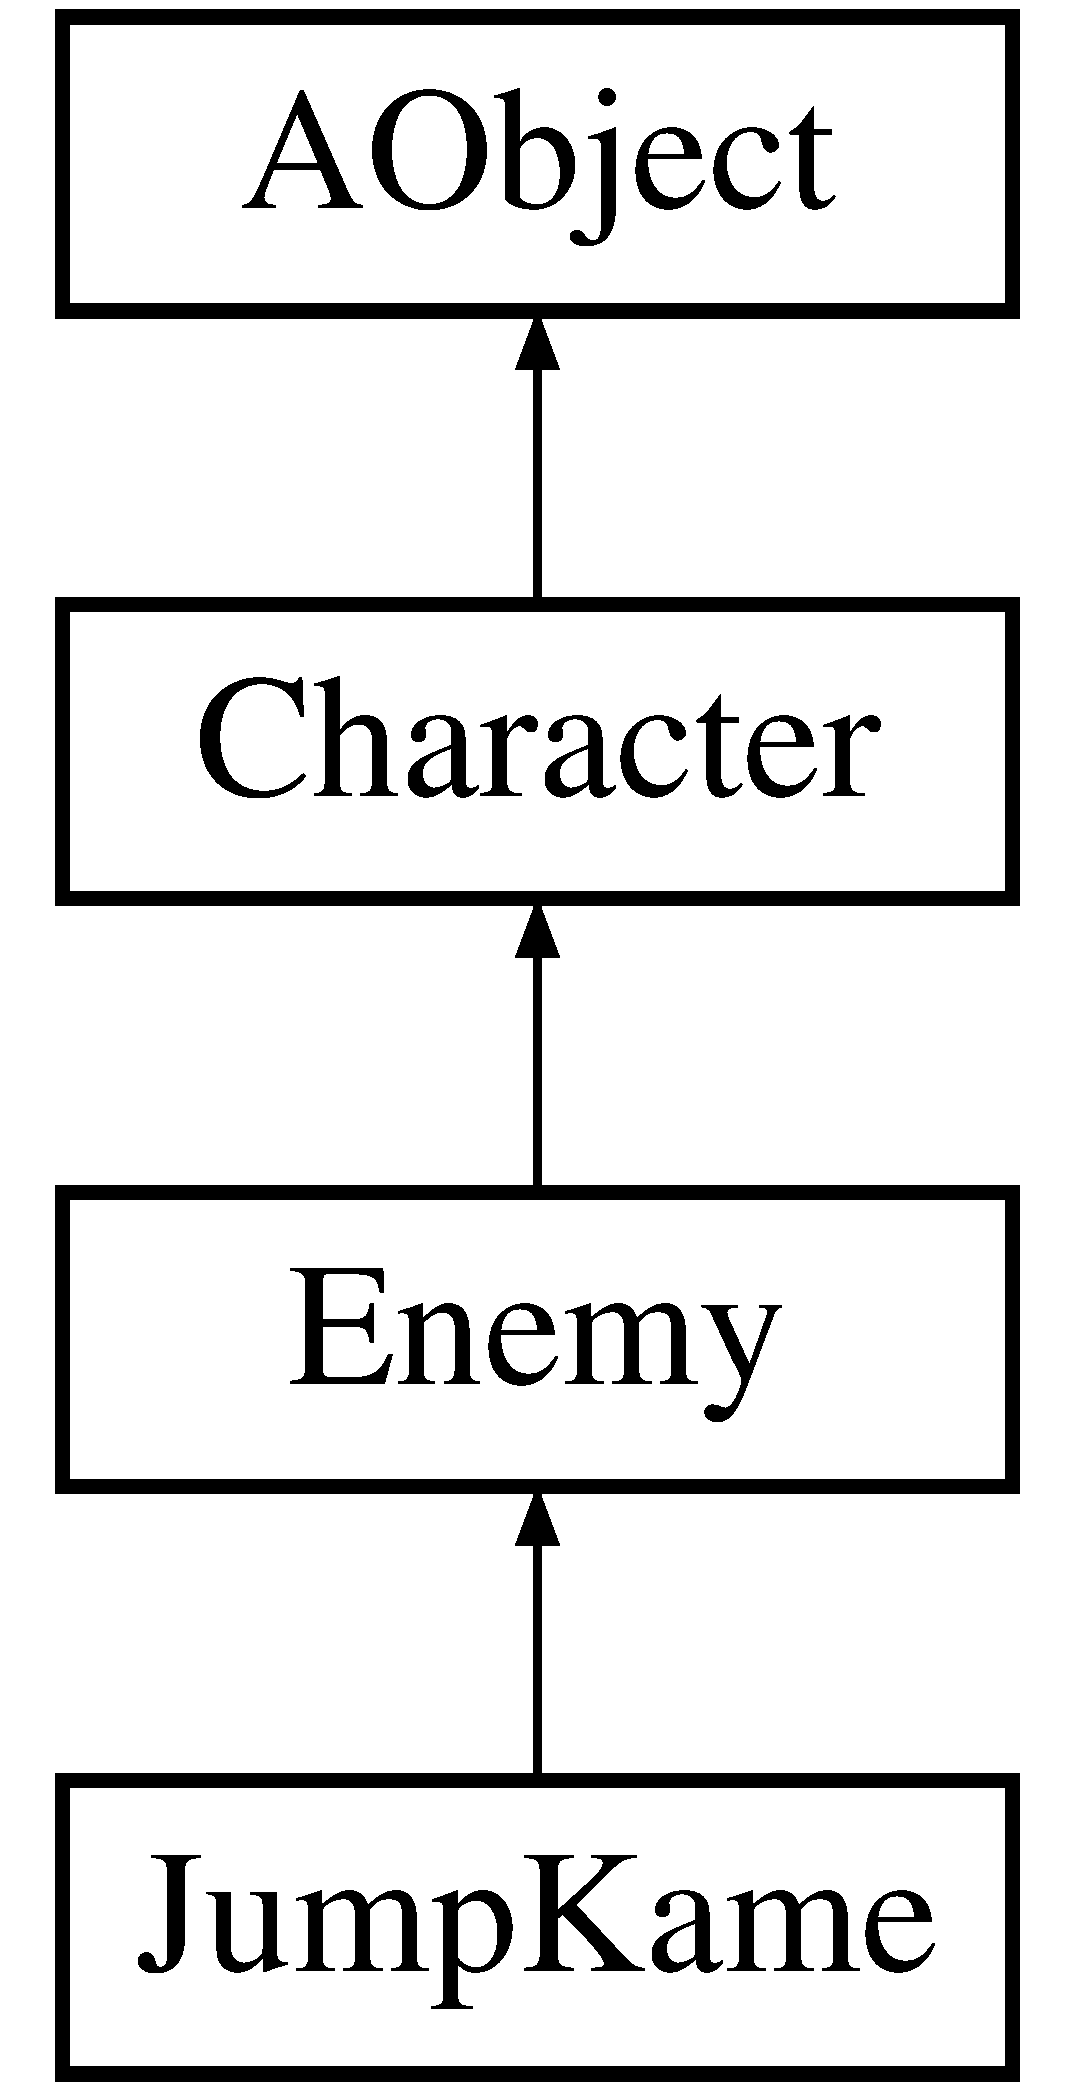
\includegraphics[height=4.000000cm]{class_jump_kame}
\end{center}
\end{figure}
\subsection*{公開メンバ関数}
\begin{DoxyCompactItemize}
\item 
\hyperlink{class_jump_kame_a2927428454b0bbd878f57f3980c3a47d}{Jump\+Kame} (double x, double y, \hyperlink{class_field}{Field} $\ast$field)
\item 
void \hyperlink{class_jump_kame_a0875bf1b86766d23294c754b63f56a0c}{Jump} ()
\end{DoxyCompactItemize}
\subsection*{非公開変数類}
\begin{DoxyCompactItemize}
\item 
int \hyperlink{class_jump_kame_a6f6699d29b773eea09aee1171b677344}{sanpo}
\end{DoxyCompactItemize}
\subsection*{その他の継承メンバ}


\subsection{構築子と解体子}
\hypertarget{class_jump_kame_a2927428454b0bbd878f57f3980c3a47d}{\index{Jump\+Kame@{Jump\+Kame}!Jump\+Kame@{Jump\+Kame}}
\index{Jump\+Kame@{Jump\+Kame}!Jump\+Kame@{Jump\+Kame}}
\subsubsection[{Jump\+Kame}]{\setlength{\rightskip}{0pt plus 5cm}Jump\+Kame\+::\+Jump\+Kame (
\begin{DoxyParamCaption}
\item[{double}]{x, }
\item[{double}]{y, }
\item[{{\bf Field} $\ast$}]{field}
\end{DoxyParamCaption}
)}}\label{class_jump_kame_a2927428454b0bbd878f57f3980c3a47d}


\subsection{関数詳解}
\hypertarget{class_jump_kame_a0875bf1b86766d23294c754b63f56a0c}{\index{Jump\+Kame@{Jump\+Kame}!Jump@{Jump}}
\index{Jump@{Jump}!Jump\+Kame@{Jump\+Kame}}
\subsubsection[{Jump}]{\setlength{\rightskip}{0pt plus 5cm}void Jump\+Kame\+::\+Jump (
\begin{DoxyParamCaption}
{}
\end{DoxyParamCaption}
)\hspace{0.3cm}{\ttfamily [virtual]}}}\label{class_jump_kame_a0875bf1b86766d23294c754b63f56a0c}


\hyperlink{class_character_a7622bdde334c8d37358218e64dd6850a}{Character}を再実装しています。



\subsection{メンバ詳解}
\hypertarget{class_jump_kame_a6f6699d29b773eea09aee1171b677344}{\index{Jump\+Kame@{Jump\+Kame}!sanpo@{sanpo}}
\index{sanpo@{sanpo}!Jump\+Kame@{Jump\+Kame}}
\subsubsection[{sanpo}]{\setlength{\rightskip}{0pt plus 5cm}int Jump\+Kame\+::sanpo\hspace{0.3cm}{\ttfamily [private]}}}\label{class_jump_kame_a6f6699d29b773eea09aee1171b677344}


このクラス詳解は次のファイルから抽出されました\+:\begin{DoxyCompactItemize}
\item 
\hyperlink{_jump_kame_8h}{Jump\+Kame.\+h}\item 
\hyperlink{_jump_kame_8cpp}{Jump\+Kame.\+cpp}\end{DoxyCompactItemize}

\hypertarget{class_kame}{\section{Kame クラス}
\label{class_kame}\index{Kame@{Kame}}
}


{\ttfamily \#include $<$Kame.\+h$>$}

Kame の継承関係図\begin{figure}[H]
\begin{center}
\leavevmode
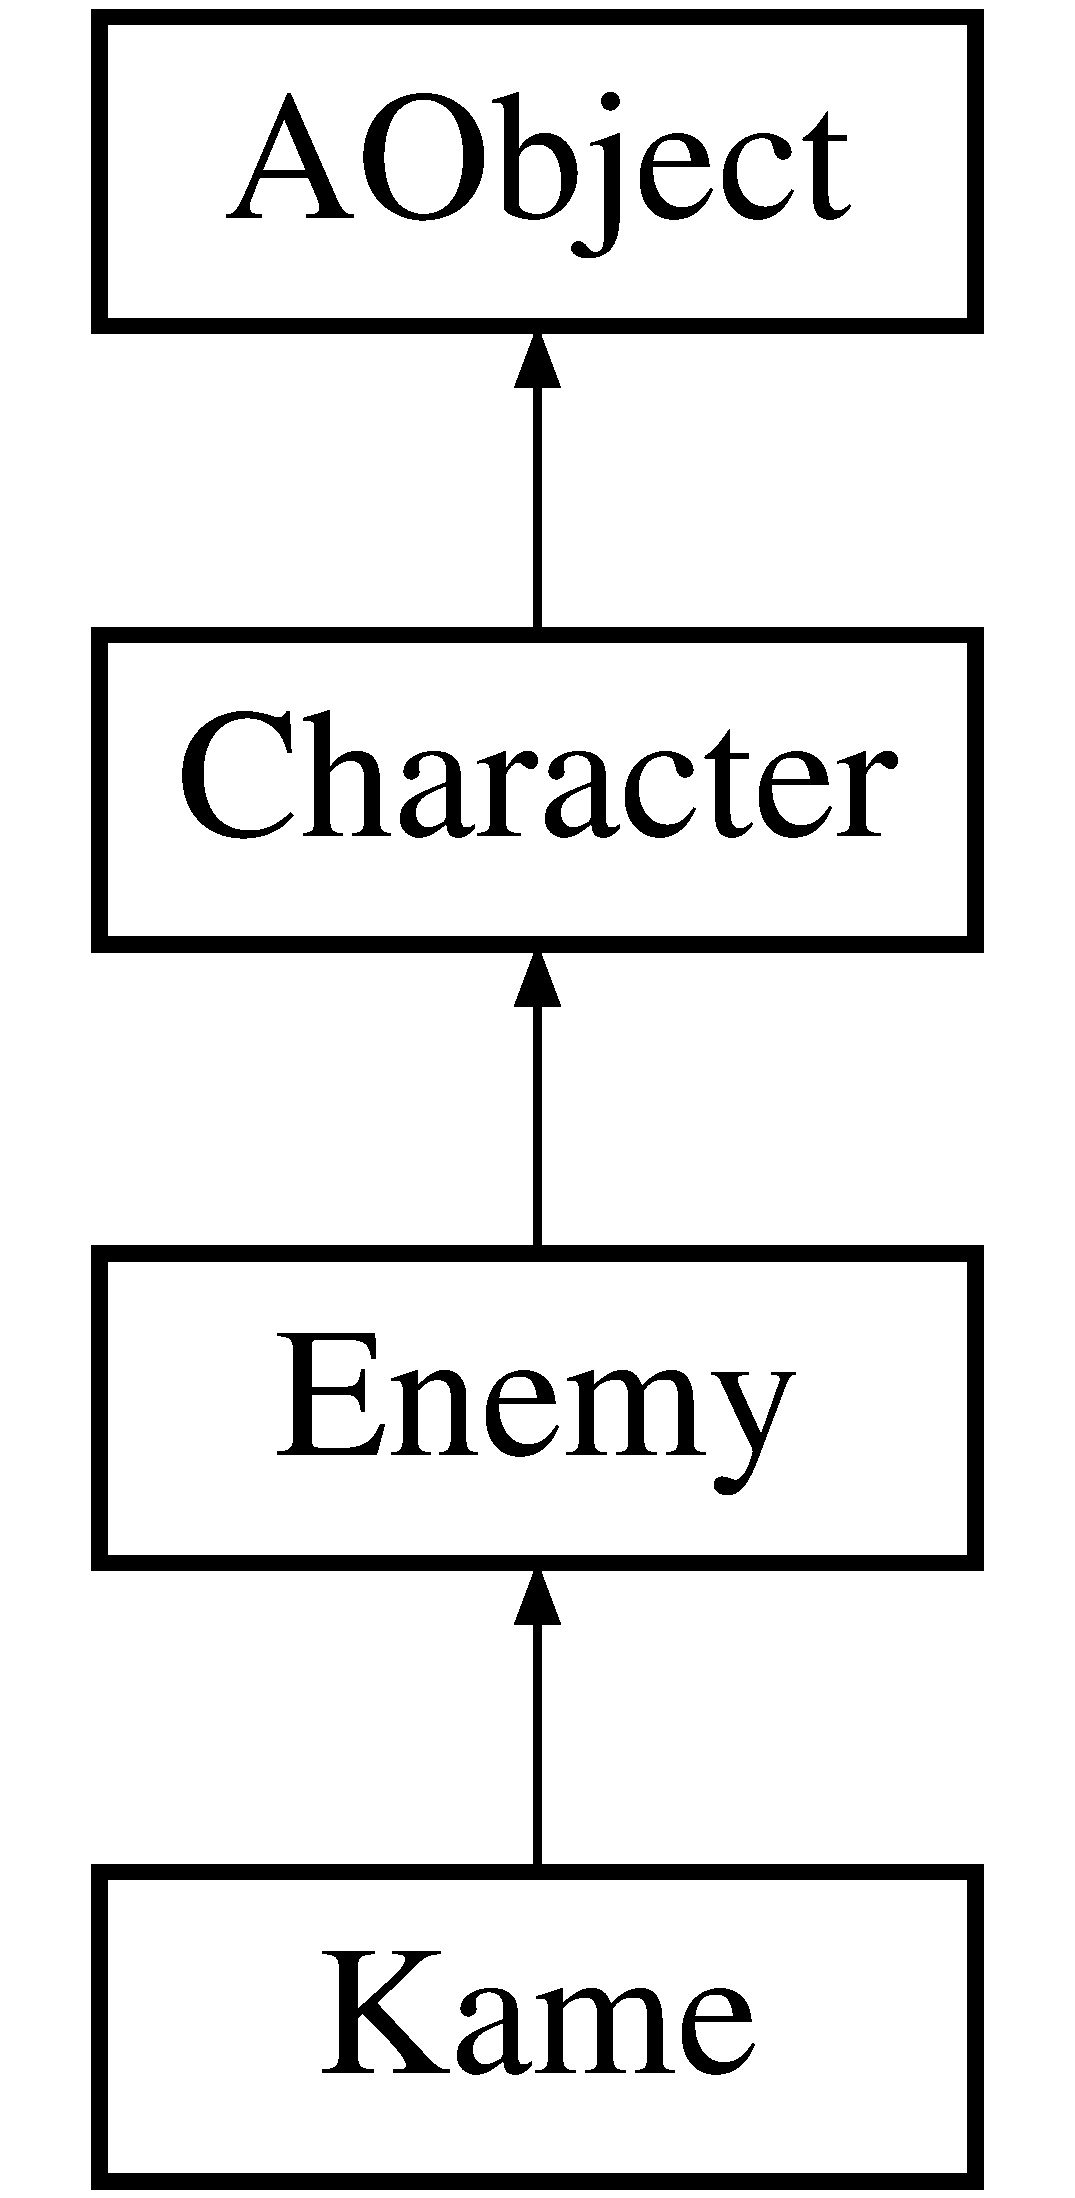
\includegraphics[height=4.000000cm]{class_kame}
\end{center}
\end{figure}
\subsection*{公開メンバ関数}
\begin{DoxyCompactItemize}
\item 
\hyperlink{class_kame_a2366fed939ec37a58e7dfbf35a58c306}{Kame} (double x, double y, \hyperlink{class_field}{Field} $\ast$field)
\end{DoxyCompactItemize}
\subsection*{その他の継承メンバ}


\subsection{構築子と解体子}
\hypertarget{class_kame_a2366fed939ec37a58e7dfbf35a58c306}{\index{Kame@{Kame}!Kame@{Kame}}
\index{Kame@{Kame}!Kame@{Kame}}
\subsubsection[{Kame}]{\setlength{\rightskip}{0pt plus 5cm}Kame\+::\+Kame (
\begin{DoxyParamCaption}
\item[{double}]{x, }
\item[{double}]{y, }
\item[{{\bf Field} $\ast$}]{field}
\end{DoxyParamCaption}
)}}\label{class_kame_a2366fed939ec37a58e7dfbf35a58c306}


このクラス詳解は次のファイルから抽出されました\+:\begin{DoxyCompactItemize}
\item 
\hyperlink{_kame_8h}{Kame.\+h}\item 
\hyperlink{_kame_8cpp}{Kame.\+cpp}\end{DoxyCompactItemize}

\hypertarget{class_load_graphic}{\section{Load\+Graphic クラス}
\label{class_load_graphic}\index{Load\+Graphic@{Load\+Graphic}}
}


{\ttfamily \#include $<$Load\+Graphic.\+h$>$}

\subsection*{公開メンバ関数}
\begin{DoxyCompactItemize}
\item 
\hyperlink{class_load_graphic_ac53171e9ee0157d8335217b9ae7259c2}{Load\+Graphic} ()
\item 
int \hyperlink{class_load_graphic_aa39fc39420113129aaf0dcdef81903bd}{Load} (char $\ast$file\+\_\+name)
\end{DoxyCompactItemize}
\subsection*{非公開変数類}
\begin{DoxyCompactItemize}
\item 
int \hyperlink{class_load_graphic_a8051a91581a0ad01f5ff8be6c2f8db65}{count}
\item 
int \hyperlink{class_load_graphic_a9756b51be935abe0d5cede28e7e5836b}{g\+\_\+handles} \mbox{[}20\mbox{]}
\item 
char $\ast$ \hyperlink{class_load_graphic_ab6fdaf84a0b4a6c6b047258417d28a16}{file\+\_\+names} \mbox{[}20\mbox{]}
\end{DoxyCompactItemize}


\subsection{構築子と解体子}
\hypertarget{class_load_graphic_ac53171e9ee0157d8335217b9ae7259c2}{\index{Load\+Graphic@{Load\+Graphic}!Load\+Graphic@{Load\+Graphic}}
\index{Load\+Graphic@{Load\+Graphic}!Load\+Graphic@{Load\+Graphic}}
\subsubsection[{Load\+Graphic}]{\setlength{\rightskip}{0pt plus 5cm}Load\+Graphic\+::\+Load\+Graphic (
\begin{DoxyParamCaption}
{}
\end{DoxyParamCaption}
)}}\label{class_load_graphic_ac53171e9ee0157d8335217b9ae7259c2}


\subsection{関数詳解}
\hypertarget{class_load_graphic_aa39fc39420113129aaf0dcdef81903bd}{\index{Load\+Graphic@{Load\+Graphic}!Load@{Load}}
\index{Load@{Load}!Load\+Graphic@{Load\+Graphic}}
\subsubsection[{Load}]{\setlength{\rightskip}{0pt plus 5cm}int Load\+Graphic\+::\+Load (
\begin{DoxyParamCaption}
\item[{char $\ast$}]{file\+\_\+name}
\end{DoxyParamCaption}
)}}\label{class_load_graphic_aa39fc39420113129aaf0dcdef81903bd}


\subsection{メンバ詳解}
\hypertarget{class_load_graphic_a8051a91581a0ad01f5ff8be6c2f8db65}{\index{Load\+Graphic@{Load\+Graphic}!count@{count}}
\index{count@{count}!Load\+Graphic@{Load\+Graphic}}
\subsubsection[{count}]{\setlength{\rightskip}{0pt plus 5cm}int Load\+Graphic\+::count\hspace{0.3cm}{\ttfamily [private]}}}\label{class_load_graphic_a8051a91581a0ad01f5ff8be6c2f8db65}
\hypertarget{class_load_graphic_ab6fdaf84a0b4a6c6b047258417d28a16}{\index{Load\+Graphic@{Load\+Graphic}!file\+\_\+names@{file\+\_\+names}}
\index{file\+\_\+names@{file\+\_\+names}!Load\+Graphic@{Load\+Graphic}}
\subsubsection[{file\+\_\+names}]{\setlength{\rightskip}{0pt plus 5cm}char$\ast$ Load\+Graphic\+::file\+\_\+names\mbox{[}20\mbox{]}\hspace{0.3cm}{\ttfamily [private]}}}\label{class_load_graphic_ab6fdaf84a0b4a6c6b047258417d28a16}
\hypertarget{class_load_graphic_a9756b51be935abe0d5cede28e7e5836b}{\index{Load\+Graphic@{Load\+Graphic}!g\+\_\+handles@{g\+\_\+handles}}
\index{g\+\_\+handles@{g\+\_\+handles}!Load\+Graphic@{Load\+Graphic}}
\subsubsection[{g\+\_\+handles}]{\setlength{\rightskip}{0pt plus 5cm}int Load\+Graphic\+::g\+\_\+handles\mbox{[}20\mbox{]}\hspace{0.3cm}{\ttfamily [private]}}}\label{class_load_graphic_a9756b51be935abe0d5cede28e7e5836b}


このクラス詳解は次のファイルから抽出されました\+:\begin{DoxyCompactItemize}
\item 
\hyperlink{_load_graphic_8h}{Load\+Graphic.\+h}\item 
\hyperlink{_load_graphic_8cpp}{Load\+Graphic.\+cpp}\end{DoxyCompactItemize}

\hypertarget{class_map}{\section{Map クラス}
\label{class_map}\index{Map@{Map}}
}


{\ttfamily \#include $<$Map.\+h$>$}

\subsection*{公開メンバ関数}
\begin{DoxyCompactItemize}
\item 
int \hyperlink{class_map_acc81681ce21cb77b686446de8054c873}{map\+\_\+width} ()
\item 
int \hyperlink{class_map_ad31ca4e58bc9aee366f4472b0d2caac0}{map\+\_\+height} ()
\item 
\hyperlink{class_map_a0f5ad0fd4563497b4214038cbca8b582}{Map} ()
\item 
\hyperlink{class_map_ae29ba970735d81d37a8c09e7e1b5a97f}{Map} (int \hyperlink{class_map_a9a14e00ff8843f4eed904f0dbe4b19dd}{cell\+\_\+width}, int \hyperlink{class_map_ad4c7bd28ec6d1b2e1e996686d5634bbc}{cell\+\_\+hegiht}, int $\ast$$\ast$\hyperlink{class_map_aebd3aa405509dae6a3a63edad08eaf63}{map\+\_\+datas})
\item 
int \hyperlink{class_map_a49a50b1bb8e6ae4f311ca730e683eae1}{Get\+Map\+Data} (double x, double y)
\item 
int \hyperlink{class_map_ae1b09990bb55f9e799a8845453975e04}{Get\+Map\+Data\+From\+Cell} (int x, int y)
\item 
void \hyperlink{class_map_a450160bcc89fd82cd1ccc7ed44c6542f}{Draw} (int offset)
\item 
void \hyperlink{class_map_a09797f6a2c27a7966f07498676080ff3}{Scroll} (int)
\item 
\hyperlink{class_map_aa403fbe09394ccf39747588f5168e3b2}{$\sim$\+Map} ()
\item 
void \hyperlink{class_map_a492de80615b6aeebb98b6b3fef47b243}{Set\+Map\+Height\+And\+Width} (int height, int width)
\end{DoxyCompactItemize}
\subsection*{非公開変数類}
\begin{DoxyCompactItemize}
\item 
int \hyperlink{class_map_aa03af329a40b2dbb4252f0a27243dcac}{background\+\_\+}
\item 
int \hyperlink{class_map_a9a14e00ff8843f4eed904f0dbe4b19dd}{cell\+\_\+width}
\item 
int \hyperlink{class_map_ad4c7bd28ec6d1b2e1e996686d5634bbc}{cell\+\_\+hegiht}
\item 
int \hyperlink{class_map_a1c47ff15c93974ddf3ef05f7bdee1571}{map\+\_\+width\+\_\+}
\item 
int \hyperlink{class_map_aaf4efb5b983ca1c0ec7e987711f57640}{map\+\_\+height\+\_\+}
\item 
int $\ast$$\ast$ \hyperlink{class_map_aebd3aa405509dae6a3a63edad08eaf63}{map\+\_\+datas}
\item 
int \hyperlink{class_map_a02557959c8b2b59592b673a356424e63}{offset\+\_\+}
\item 
int \hyperlink{class_map_a3d03c3930a3d2d4c9d7609ae46a730ea}{wall\+Graph\+\_\+}
\end{DoxyCompactItemize}


\subsection{構築子と解体子}
\hypertarget{class_map_a0f5ad0fd4563497b4214038cbca8b582}{\index{Map@{Map}!Map@{Map}}
\index{Map@{Map}!Map@{Map}}
\subsubsection[{Map}]{\setlength{\rightskip}{0pt plus 5cm}Map\+::\+Map (
\begin{DoxyParamCaption}
{}
\end{DoxyParamCaption}
)}}\label{class_map_a0f5ad0fd4563497b4214038cbca8b582}
\hypertarget{class_map_ae29ba970735d81d37a8c09e7e1b5a97f}{\index{Map@{Map}!Map@{Map}}
\index{Map@{Map}!Map@{Map}}
\subsubsection[{Map}]{\setlength{\rightskip}{0pt plus 5cm}Map\+::\+Map (
\begin{DoxyParamCaption}
\item[{int}]{cell\+\_\+width, }
\item[{int}]{cell\+\_\+hegiht, }
\item[{int $\ast$$\ast$}]{map\+\_\+datas}
\end{DoxyParamCaption}
)}}\label{class_map_ae29ba970735d81d37a8c09e7e1b5a97f}
\hypertarget{class_map_aa403fbe09394ccf39747588f5168e3b2}{\index{Map@{Map}!````~Map@{$\sim$\+Map}}
\index{````~Map@{$\sim$\+Map}!Map@{Map}}
\subsubsection[{$\sim$\+Map}]{\setlength{\rightskip}{0pt plus 5cm}Map\+::$\sim$\+Map (
\begin{DoxyParamCaption}
{}
\end{DoxyParamCaption}
)}}\label{class_map_aa403fbe09394ccf39747588f5168e3b2}


\subsection{関数詳解}
\hypertarget{class_map_a450160bcc89fd82cd1ccc7ed44c6542f}{\index{Map@{Map}!Draw@{Draw}}
\index{Draw@{Draw}!Map@{Map}}
\subsubsection[{Draw}]{\setlength{\rightskip}{0pt plus 5cm}void Map\+::\+Draw (
\begin{DoxyParamCaption}
\item[{int}]{offset}
\end{DoxyParamCaption}
)}}\label{class_map_a450160bcc89fd82cd1ccc7ed44c6542f}
\hypertarget{class_map_a49a50b1bb8e6ae4f311ca730e683eae1}{\index{Map@{Map}!Get\+Map\+Data@{Get\+Map\+Data}}
\index{Get\+Map\+Data@{Get\+Map\+Data}!Map@{Map}}
\subsubsection[{Get\+Map\+Data}]{\setlength{\rightskip}{0pt plus 5cm}int Map\+::\+Get\+Map\+Data (
\begin{DoxyParamCaption}
\item[{double}]{x, }
\item[{double}]{y}
\end{DoxyParamCaption}
)}}\label{class_map_a49a50b1bb8e6ae4f311ca730e683eae1}
\hypertarget{class_map_ae1b09990bb55f9e799a8845453975e04}{\index{Map@{Map}!Get\+Map\+Data\+From\+Cell@{Get\+Map\+Data\+From\+Cell}}
\index{Get\+Map\+Data\+From\+Cell@{Get\+Map\+Data\+From\+Cell}!Map@{Map}}
\subsubsection[{Get\+Map\+Data\+From\+Cell}]{\setlength{\rightskip}{0pt plus 5cm}int Map\+::\+Get\+Map\+Data\+From\+Cell (
\begin{DoxyParamCaption}
\item[{int}]{x, }
\item[{int}]{y}
\end{DoxyParamCaption}
)}}\label{class_map_ae1b09990bb55f9e799a8845453975e04}
\hypertarget{class_map_ad31ca4e58bc9aee366f4472b0d2caac0}{\index{Map@{Map}!map\+\_\+height@{map\+\_\+height}}
\index{map\+\_\+height@{map\+\_\+height}!Map@{Map}}
\subsubsection[{map\+\_\+height}]{\setlength{\rightskip}{0pt plus 5cm}int Map\+::map\+\_\+height (
\begin{DoxyParamCaption}
{}
\end{DoxyParamCaption}
)\hspace{0.3cm}{\ttfamily [inline]}}}\label{class_map_ad31ca4e58bc9aee366f4472b0d2caac0}
\hypertarget{class_map_acc81681ce21cb77b686446de8054c873}{\index{Map@{Map}!map\+\_\+width@{map\+\_\+width}}
\index{map\+\_\+width@{map\+\_\+width}!Map@{Map}}
\subsubsection[{map\+\_\+width}]{\setlength{\rightskip}{0pt plus 5cm}int Map\+::map\+\_\+width (
\begin{DoxyParamCaption}
{}
\end{DoxyParamCaption}
)\hspace{0.3cm}{\ttfamily [inline]}}}\label{class_map_acc81681ce21cb77b686446de8054c873}
\hypertarget{class_map_a09797f6a2c27a7966f07498676080ff3}{\index{Map@{Map}!Scroll@{Scroll}}
\index{Scroll@{Scroll}!Map@{Map}}
\subsubsection[{Scroll}]{\setlength{\rightskip}{0pt plus 5cm}void Map\+::\+Scroll (
\begin{DoxyParamCaption}
\item[{int}]{move}
\end{DoxyParamCaption}
)}}\label{class_map_a09797f6a2c27a7966f07498676080ff3}
\hypertarget{class_map_a492de80615b6aeebb98b6b3fef47b243}{\index{Map@{Map}!Set\+Map\+Height\+And\+Width@{Set\+Map\+Height\+And\+Width}}
\index{Set\+Map\+Height\+And\+Width@{Set\+Map\+Height\+And\+Width}!Map@{Map}}
\subsubsection[{Set\+Map\+Height\+And\+Width}]{\setlength{\rightskip}{0pt plus 5cm}void Map\+::\+Set\+Map\+Height\+And\+Width (
\begin{DoxyParamCaption}
\item[{int}]{height, }
\item[{int}]{width}
\end{DoxyParamCaption}
)}}\label{class_map_a492de80615b6aeebb98b6b3fef47b243}


\subsection{メンバ詳解}
\hypertarget{class_map_aa03af329a40b2dbb4252f0a27243dcac}{\index{Map@{Map}!background\+\_\+@{background\+\_\+}}
\index{background\+\_\+@{background\+\_\+}!Map@{Map}}
\subsubsection[{background\+\_\+}]{\setlength{\rightskip}{0pt plus 5cm}int Map\+::background\+\_\+\hspace{0.3cm}{\ttfamily [private]}}}\label{class_map_aa03af329a40b2dbb4252f0a27243dcac}
\hypertarget{class_map_ad4c7bd28ec6d1b2e1e996686d5634bbc}{\index{Map@{Map}!cell\+\_\+hegiht@{cell\+\_\+hegiht}}
\index{cell\+\_\+hegiht@{cell\+\_\+hegiht}!Map@{Map}}
\subsubsection[{cell\+\_\+hegiht}]{\setlength{\rightskip}{0pt plus 5cm}int Map\+::cell\+\_\+hegiht\hspace{0.3cm}{\ttfamily [private]}}}\label{class_map_ad4c7bd28ec6d1b2e1e996686d5634bbc}
\hypertarget{class_map_a9a14e00ff8843f4eed904f0dbe4b19dd}{\index{Map@{Map}!cell\+\_\+width@{cell\+\_\+width}}
\index{cell\+\_\+width@{cell\+\_\+width}!Map@{Map}}
\subsubsection[{cell\+\_\+width}]{\setlength{\rightskip}{0pt plus 5cm}int Map\+::cell\+\_\+width\hspace{0.3cm}{\ttfamily [private]}}}\label{class_map_a9a14e00ff8843f4eed904f0dbe4b19dd}
\hypertarget{class_map_aebd3aa405509dae6a3a63edad08eaf63}{\index{Map@{Map}!map\+\_\+datas@{map\+\_\+datas}}
\index{map\+\_\+datas@{map\+\_\+datas}!Map@{Map}}
\subsubsection[{map\+\_\+datas}]{\setlength{\rightskip}{0pt plus 5cm}int$\ast$$\ast$ Map\+::map\+\_\+datas\hspace{0.3cm}{\ttfamily [private]}}}\label{class_map_aebd3aa405509dae6a3a63edad08eaf63}
\hypertarget{class_map_aaf4efb5b983ca1c0ec7e987711f57640}{\index{Map@{Map}!map\+\_\+height\+\_\+@{map\+\_\+height\+\_\+}}
\index{map\+\_\+height\+\_\+@{map\+\_\+height\+\_\+}!Map@{Map}}
\subsubsection[{map\+\_\+height\+\_\+}]{\setlength{\rightskip}{0pt plus 5cm}int Map\+::map\+\_\+height\+\_\+\hspace{0.3cm}{\ttfamily [private]}}}\label{class_map_aaf4efb5b983ca1c0ec7e987711f57640}
\hypertarget{class_map_a1c47ff15c93974ddf3ef05f7bdee1571}{\index{Map@{Map}!map\+\_\+width\+\_\+@{map\+\_\+width\+\_\+}}
\index{map\+\_\+width\+\_\+@{map\+\_\+width\+\_\+}!Map@{Map}}
\subsubsection[{map\+\_\+width\+\_\+}]{\setlength{\rightskip}{0pt plus 5cm}int Map\+::map\+\_\+width\+\_\+\hspace{0.3cm}{\ttfamily [private]}}}\label{class_map_a1c47ff15c93974ddf3ef05f7bdee1571}
\hypertarget{class_map_a02557959c8b2b59592b673a356424e63}{\index{Map@{Map}!offset\+\_\+@{offset\+\_\+}}
\index{offset\+\_\+@{offset\+\_\+}!Map@{Map}}
\subsubsection[{offset\+\_\+}]{\setlength{\rightskip}{0pt plus 5cm}int Map\+::offset\+\_\+\hspace{0.3cm}{\ttfamily [private]}}}\label{class_map_a02557959c8b2b59592b673a356424e63}
\hypertarget{class_map_a3d03c3930a3d2d4c9d7609ae46a730ea}{\index{Map@{Map}!wall\+Graph\+\_\+@{wall\+Graph\+\_\+}}
\index{wall\+Graph\+\_\+@{wall\+Graph\+\_\+}!Map@{Map}}
\subsubsection[{wall\+Graph\+\_\+}]{\setlength{\rightskip}{0pt plus 5cm}int Map\+::wall\+Graph\+\_\+\hspace{0.3cm}{\ttfamily [private]}}}\label{class_map_a3d03c3930a3d2d4c9d7609ae46a730ea}


このクラス詳解は次のファイルから抽出されました\+:\begin{DoxyCompactItemize}
\item 
\hyperlink{_map_8h}{Map.\+h}\item 
\hyperlink{_map_8cpp}{Map.\+cpp}\end{DoxyCompactItemize}

\hypertarget{class_map_factory}{\section{Map\+Factory クラス}
\label{class_map_factory}\index{Map\+Factory@{Map\+Factory}}
}


{\ttfamily \#include $<$Map\+Factory.\+h$>$}

\subsection*{公開メンバ関数}
\begin{DoxyCompactItemize}
\item 
\hyperlink{class_map}{Map} $\ast$ \hyperlink{class_map_factory_aa74eff81af5352393ab5016efa249c0d}{Create\+Map} (std\+::string file\+Name)
\end{DoxyCompactItemize}


\subsection{関数詳解}
\hypertarget{class_map_factory_aa74eff81af5352393ab5016efa249c0d}{\index{Map\+Factory@{Map\+Factory}!Create\+Map@{Create\+Map}}
\index{Create\+Map@{Create\+Map}!Map\+Factory@{Map\+Factory}}
\subsubsection[{Create\+Map}]{\setlength{\rightskip}{0pt plus 5cm}{\bf Map} $\ast$ Map\+Factory\+::\+Create\+Map (
\begin{DoxyParamCaption}
\item[{std\+::string}]{file\+Name}
\end{DoxyParamCaption}
)}}\label{class_map_factory_aa74eff81af5352393ab5016efa249c0d}


このクラス詳解は次のファイルから抽出されました\+:\begin{DoxyCompactItemize}
\item 
\hyperlink{_map_factory_8h}{Map\+Factory.\+h}\item 
\hyperlink{_map_factory_8cpp}{Map\+Factory.\+cpp}\end{DoxyCompactItemize}

\hypertarget{class_menu}{\section{Menu クラス}
\label{class_menu}\index{Menu@{Menu}}
}


{\ttfamily \#include $<$Menu.\+h$>$}

\subsection*{クラス}
\begin{DoxyCompactItemize}
\item 
struct \hyperlink{struct_menu_1_1_menu_element__t}{Menu\+Element\+\_\+t}
\end{DoxyCompactItemize}
\subsection*{公開メンバ関数}
\begin{DoxyCompactItemize}
\item 
void \hyperlink{class_menu_af24259cfce6f1beeb1e547735c3126be}{Start} ()
\item 
string \hyperlink{class_menu_a0c448739883a9e61e4ddd52ffde097da}{Select} ()
\item 
int \hyperlink{class_menu_a23303ace170484ab0663b18f75156df1}{gp\+Update\+Key} ()
\end{DoxyCompactItemize}
\subsection*{非公開変数類}
\begin{DoxyCompactItemize}
\item 
int \hyperlink{class_menu_a6a356e223f85e7957ffba91bdf634a56}{key} \mbox{[}256\mbox{]}
\end{DoxyCompactItemize}


\subsection{関数詳解}
\hypertarget{class_menu_a23303ace170484ab0663b18f75156df1}{\index{Menu@{Menu}!gp\+Update\+Key@{gp\+Update\+Key}}
\index{gp\+Update\+Key@{gp\+Update\+Key}!Menu@{Menu}}
\subsubsection[{gp\+Update\+Key}]{\setlength{\rightskip}{0pt plus 5cm}int Menu\+::gp\+Update\+Key (
\begin{DoxyParamCaption}
{}
\end{DoxyParamCaption}
)}}\label{class_menu_a23303ace170484ab0663b18f75156df1}
\hypertarget{class_menu_a0c448739883a9e61e4ddd52ffde097da}{\index{Menu@{Menu}!Select@{Select}}
\index{Select@{Select}!Menu@{Menu}}
\subsubsection[{Select}]{\setlength{\rightskip}{0pt plus 5cm}string Menu\+::\+Select (
\begin{DoxyParamCaption}
{}
\end{DoxyParamCaption}
)}}\label{class_menu_a0c448739883a9e61e4ddd52ffde097da}
\hypertarget{class_menu_af24259cfce6f1beeb1e547735c3126be}{\index{Menu@{Menu}!Start@{Start}}
\index{Start@{Start}!Menu@{Menu}}
\subsubsection[{Start}]{\setlength{\rightskip}{0pt plus 5cm}void Menu\+::\+Start (
\begin{DoxyParamCaption}
{}
\end{DoxyParamCaption}
)}}\label{class_menu_af24259cfce6f1beeb1e547735c3126be}


\subsection{メンバ詳解}
\hypertarget{class_menu_a6a356e223f85e7957ffba91bdf634a56}{\index{Menu@{Menu}!key@{key}}
\index{key@{key}!Menu@{Menu}}
\subsubsection[{key}]{\setlength{\rightskip}{0pt plus 5cm}int Menu\+::key\mbox{[}256\mbox{]}\hspace{0.3cm}{\ttfamily [private]}}}\label{class_menu_a6a356e223f85e7957ffba91bdf634a56}


このクラス詳解は次のファイルから抽出されました\+:\begin{DoxyCompactItemize}
\item 
\hyperlink{_menu_8h}{Menu.\+h}\item 
\hyperlink{_menu_8cpp}{Menu.\+cpp}\end{DoxyCompactItemize}

\hypertarget{struct_menu_1_1_menu_element__t}{\section{Menu\+:\+:Menu\+Element\+\_\+t 構造体}
\label{struct_menu_1_1_menu_element__t}\index{Menu\+::\+Menu\+Element\+\_\+t@{Menu\+::\+Menu\+Element\+\_\+t}}
}
\subsection*{公開変数類}
\begin{DoxyCompactItemize}
\item 
int \hyperlink{struct_menu_1_1_menu_element__t_a32951f293ee164b34c17d78f430ff4df}{x}
\item 
int \hyperlink{struct_menu_1_1_menu_element__t_a2d2fd0d65e8c8d9bdbf43bd9647b99c9}{y}
\item 
char \hyperlink{struct_menu_1_1_menu_element__t_aba2866f80e22a37cb7657e5344308b2b}{pic\+Name} \mbox{[}128\mbox{]}
\item 
char \hyperlink{struct_menu_1_1_menu_element__t_ab24c449e97323b9f4e91d1e8e19db008}{file\+Name} \mbox{[}128\mbox{]}
\end{DoxyCompactItemize}


\subsection{メンバ詳解}
\hypertarget{struct_menu_1_1_menu_element__t_ab24c449e97323b9f4e91d1e8e19db008}{\index{Menu\+::\+Menu\+Element\+\_\+t@{Menu\+::\+Menu\+Element\+\_\+t}!file\+Name@{file\+Name}}
\index{file\+Name@{file\+Name}!Menu\+::\+Menu\+Element\+\_\+t@{Menu\+::\+Menu\+Element\+\_\+t}}
\subsubsection[{file\+Name}]{\setlength{\rightskip}{0pt plus 5cm}char Menu\+::\+Menu\+Element\+\_\+t\+::file\+Name\mbox{[}128\mbox{]}}}\label{struct_menu_1_1_menu_element__t_ab24c449e97323b9f4e91d1e8e19db008}
\hypertarget{struct_menu_1_1_menu_element__t_aba2866f80e22a37cb7657e5344308b2b}{\index{Menu\+::\+Menu\+Element\+\_\+t@{Menu\+::\+Menu\+Element\+\_\+t}!pic\+Name@{pic\+Name}}
\index{pic\+Name@{pic\+Name}!Menu\+::\+Menu\+Element\+\_\+t@{Menu\+::\+Menu\+Element\+\_\+t}}
\subsubsection[{pic\+Name}]{\setlength{\rightskip}{0pt plus 5cm}char Menu\+::\+Menu\+Element\+\_\+t\+::pic\+Name\mbox{[}128\mbox{]}}}\label{struct_menu_1_1_menu_element__t_aba2866f80e22a37cb7657e5344308b2b}
\hypertarget{struct_menu_1_1_menu_element__t_a32951f293ee164b34c17d78f430ff4df}{\index{Menu\+::\+Menu\+Element\+\_\+t@{Menu\+::\+Menu\+Element\+\_\+t}!x@{x}}
\index{x@{x}!Menu\+::\+Menu\+Element\+\_\+t@{Menu\+::\+Menu\+Element\+\_\+t}}
\subsubsection[{x}]{\setlength{\rightskip}{0pt plus 5cm}int Menu\+::\+Menu\+Element\+\_\+t\+::x}}\label{struct_menu_1_1_menu_element__t_a32951f293ee164b34c17d78f430ff4df}
\hypertarget{struct_menu_1_1_menu_element__t_a2d2fd0d65e8c8d9bdbf43bd9647b99c9}{\index{Menu\+::\+Menu\+Element\+\_\+t@{Menu\+::\+Menu\+Element\+\_\+t}!y@{y}}
\index{y@{y}!Menu\+::\+Menu\+Element\+\_\+t@{Menu\+::\+Menu\+Element\+\_\+t}}
\subsubsection[{y}]{\setlength{\rightskip}{0pt plus 5cm}int Menu\+::\+Menu\+Element\+\_\+t\+::y}}\label{struct_menu_1_1_menu_element__t_a2d2fd0d65e8c8d9bdbf43bd9647b99c9}


この構造体詳解は次のファイルから抽出されました\+:\begin{DoxyCompactItemize}
\item 
\hyperlink{_menu_8h}{Menu.\+h}\end{DoxyCompactItemize}

\hypertarget{class_no_attack}{\section{No\+Attack クラス}
\label{class_no_attack}\index{No\+Attack@{No\+Attack}}
}


{\ttfamily \#include $<$No\+Attack.\+h$>$}

No\+Attack の継承関係図\begin{figure}[H]
\begin{center}
\leavevmode
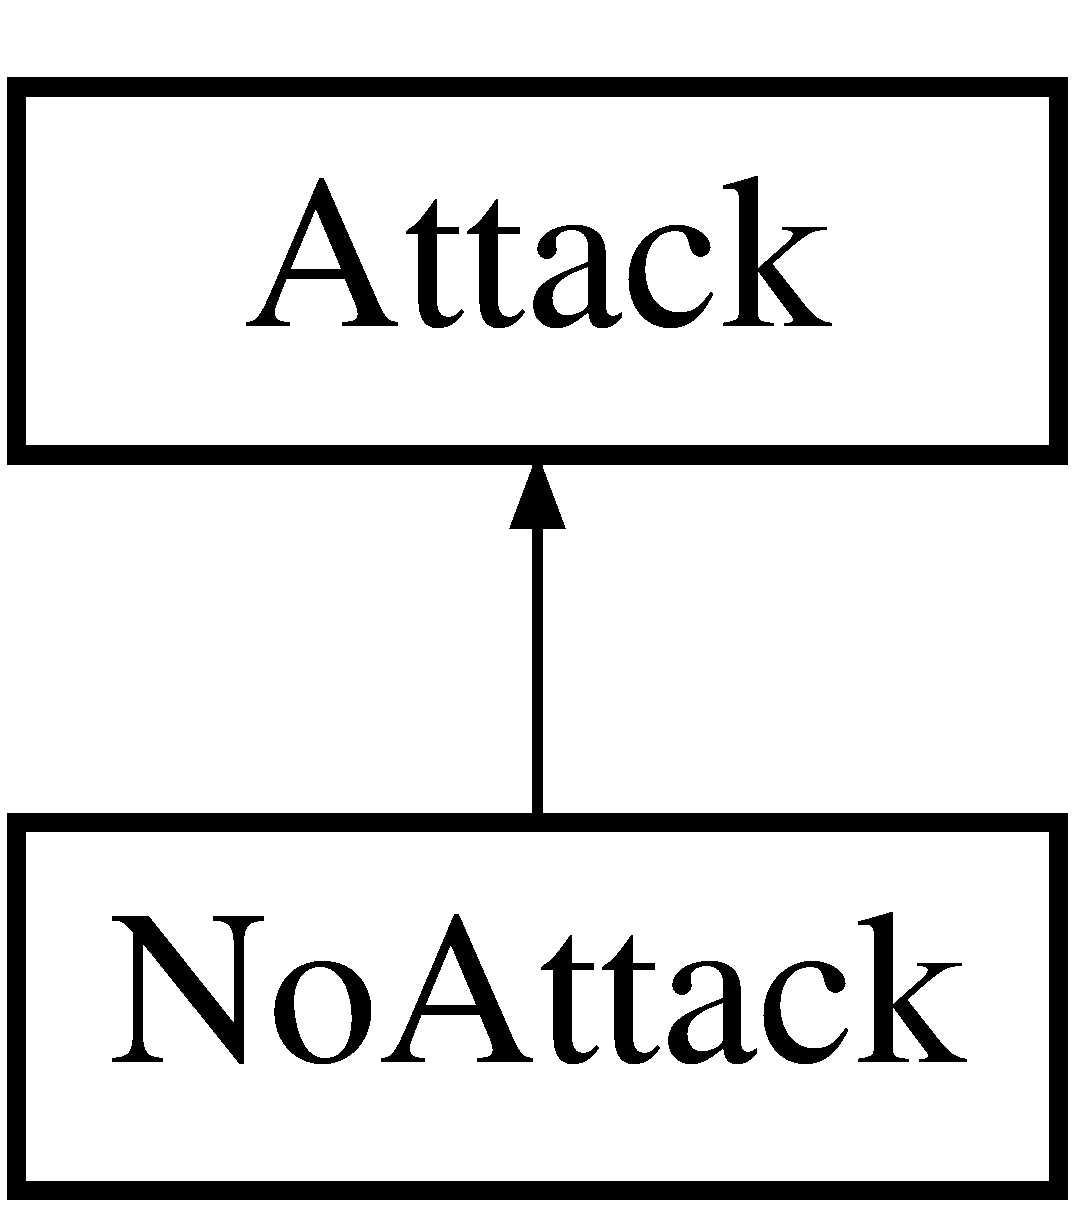
\includegraphics[height=2.000000cm]{class_no_attack}
\end{center}
\end{figure}
\subsection*{公開メンバ関数}
\begin{DoxyCompactItemize}
\item 
\hyperlink{class_no_attack_a2835d4b513feaaedf654abbd0dabe210}{No\+Attack} (\hyperlink{class_character}{Character} $\ast$chara)
\item 
void \hyperlink{class_no_attack_a42e89327c50ecc690056bf5c605a898b}{Do\+Attack} ()
\item 
void \hyperlink{class_no_attack_a183ab68341fef13f86ea3ef020a53546}{Initialize\+Bullet} (int num)
\item 
\hyperlink{class_no_attack_aec116619d17b704addb41a844062dacd}{$\sim$\+No\+Attack} (void)
\end{DoxyCompactItemize}
\subsection*{その他の継承メンバ}


\subsection{構築子と解体子}
\hypertarget{class_no_attack_a2835d4b513feaaedf654abbd0dabe210}{\index{No\+Attack@{No\+Attack}!No\+Attack@{No\+Attack}}
\index{No\+Attack@{No\+Attack}!No\+Attack@{No\+Attack}}
\subsubsection[{No\+Attack}]{\setlength{\rightskip}{0pt plus 5cm}No\+Attack\+::\+No\+Attack (
\begin{DoxyParamCaption}
\item[{{\bf Character} $\ast$}]{chara}
\end{DoxyParamCaption}
)}}\label{class_no_attack_a2835d4b513feaaedf654abbd0dabe210}
\hypertarget{class_no_attack_aec116619d17b704addb41a844062dacd}{\index{No\+Attack@{No\+Attack}!````~No\+Attack@{$\sim$\+No\+Attack}}
\index{````~No\+Attack@{$\sim$\+No\+Attack}!No\+Attack@{No\+Attack}}
\subsubsection[{$\sim$\+No\+Attack}]{\setlength{\rightskip}{0pt plus 5cm}No\+Attack\+::$\sim$\+No\+Attack (
\begin{DoxyParamCaption}
\item[{void}]{}
\end{DoxyParamCaption}
)}}\label{class_no_attack_aec116619d17b704addb41a844062dacd}


\subsection{関数詳解}
\hypertarget{class_no_attack_a42e89327c50ecc690056bf5c605a898b}{\index{No\+Attack@{No\+Attack}!Do\+Attack@{Do\+Attack}}
\index{Do\+Attack@{Do\+Attack}!No\+Attack@{No\+Attack}}
\subsubsection[{Do\+Attack}]{\setlength{\rightskip}{0pt plus 5cm}void No\+Attack\+::\+Do\+Attack (
\begin{DoxyParamCaption}
{}
\end{DoxyParamCaption}
)\hspace{0.3cm}{\ttfamily [virtual]}}}\label{class_no_attack_a42e89327c50ecc690056bf5c605a898b}


\hyperlink{class_attack_a06d145ff7c11cfef2b688eefcd11dac1}{Attack}を実装しています。

\hypertarget{class_no_attack_a183ab68341fef13f86ea3ef020a53546}{\index{No\+Attack@{No\+Attack}!Initialize\+Bullet@{Initialize\+Bullet}}
\index{Initialize\+Bullet@{Initialize\+Bullet}!No\+Attack@{No\+Attack}}
\subsubsection[{Initialize\+Bullet}]{\setlength{\rightskip}{0pt plus 5cm}void No\+Attack\+::\+Initialize\+Bullet (
\begin{DoxyParamCaption}
\item[{int}]{num}
\end{DoxyParamCaption}
)\hspace{0.3cm}{\ttfamily [virtual]}}}\label{class_no_attack_a183ab68341fef13f86ea3ef020a53546}


\hyperlink{class_attack_ac02b84493ca19adf8425c1ed2efaf54c}{Attack}を実装しています。



このクラス詳解は次のファイルから抽出されました\+:\begin{DoxyCompactItemize}
\item 
\hyperlink{_no_attack_8h}{No\+Attack.\+h}\item 
\hyperlink{_no_attack_8cpp}{No\+Attack.\+cpp}\end{DoxyCompactItemize}

\hypertarget{class_normal_attack}{\section{Normal\+Attack クラス}
\label{class_normal_attack}\index{Normal\+Attack@{Normal\+Attack}}
}


{\ttfamily \#include $<$Normal\+Attack.\+h$>$}

Normal\+Attack の継承関係図\begin{figure}[H]
\begin{center}
\leavevmode
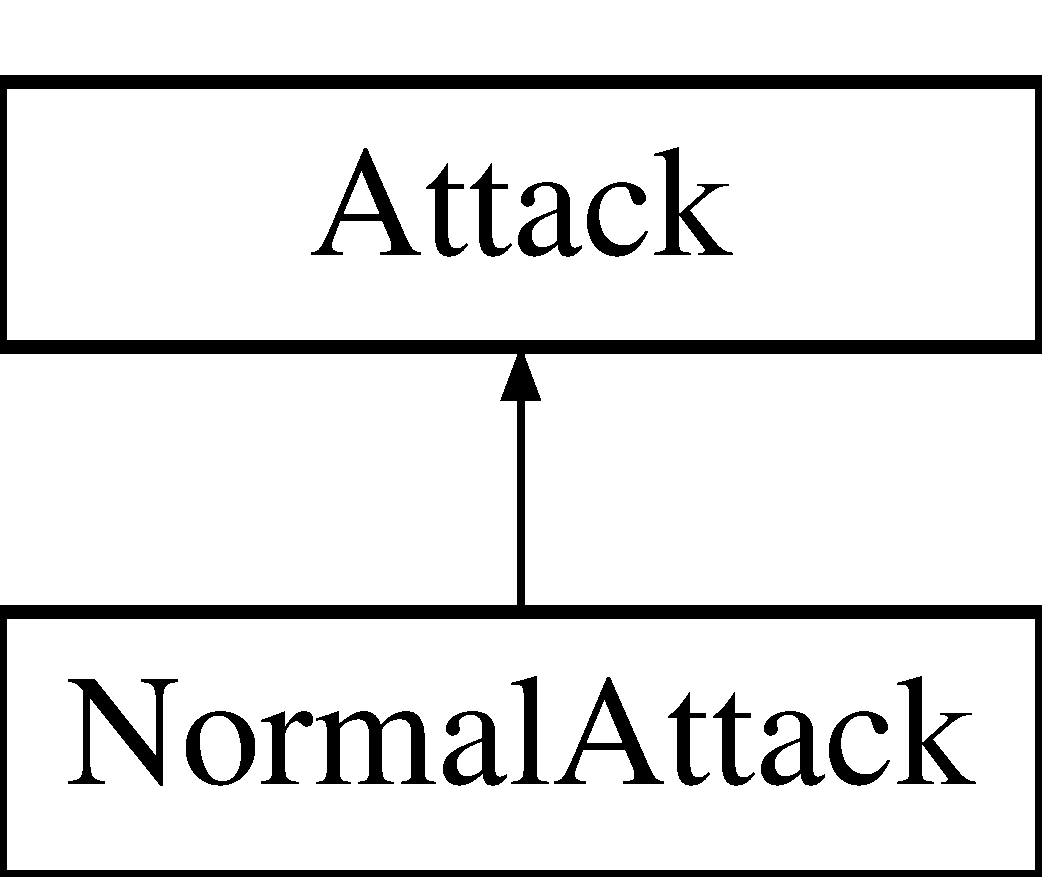
\includegraphics[height=2.000000cm]{class_normal_attack}
\end{center}
\end{figure}
\subsection*{公開メンバ関数}
\begin{DoxyCompactItemize}
\item 
\hyperlink{class_normal_attack_aef592f0fdd9752de416b82f0c076a0b1}{Normal\+Attack} (int damage, int speed, int interval, \hyperlink{class_character}{Character} $\ast$chara)
\item 
void \hyperlink{class_normal_attack_a39d8e90194dca1a89ba961163b7d0e18}{Do\+Attack} ()
\item 
void \hyperlink{class_normal_attack_a95c5acd8739229d71395a8423c32a455}{Initialize\+Bullet} (int num)
\item 
\hyperlink{class_normal_attack_a61caca3c8aa81ecfa576fb86e4032964}{$\sim$\+Normal\+Attack} (void)
\end{DoxyCompactItemize}
\subsection*{その他の継承メンバ}


\subsection{構築子と解体子}
\hypertarget{class_normal_attack_aef592f0fdd9752de416b82f0c076a0b1}{\index{Normal\+Attack@{Normal\+Attack}!Normal\+Attack@{Normal\+Attack}}
\index{Normal\+Attack@{Normal\+Attack}!Normal\+Attack@{Normal\+Attack}}
\subsubsection[{Normal\+Attack}]{\setlength{\rightskip}{0pt plus 5cm}Normal\+Attack\+::\+Normal\+Attack (
\begin{DoxyParamCaption}
\item[{int}]{damage, }
\item[{int}]{speed, }
\item[{int}]{interval, }
\item[{{\bf Character} $\ast$}]{chara}
\end{DoxyParamCaption}
)}}\label{class_normal_attack_aef592f0fdd9752de416b82f0c076a0b1}
\hypertarget{class_normal_attack_a61caca3c8aa81ecfa576fb86e4032964}{\index{Normal\+Attack@{Normal\+Attack}!````~Normal\+Attack@{$\sim$\+Normal\+Attack}}
\index{````~Normal\+Attack@{$\sim$\+Normal\+Attack}!Normal\+Attack@{Normal\+Attack}}
\subsubsection[{$\sim$\+Normal\+Attack}]{\setlength{\rightskip}{0pt plus 5cm}Normal\+Attack\+::$\sim$\+Normal\+Attack (
\begin{DoxyParamCaption}
\item[{void}]{}
\end{DoxyParamCaption}
)}}\label{class_normal_attack_a61caca3c8aa81ecfa576fb86e4032964}


\subsection{関数詳解}
\hypertarget{class_normal_attack_a39d8e90194dca1a89ba961163b7d0e18}{\index{Normal\+Attack@{Normal\+Attack}!Do\+Attack@{Do\+Attack}}
\index{Do\+Attack@{Do\+Attack}!Normal\+Attack@{Normal\+Attack}}
\subsubsection[{Do\+Attack}]{\setlength{\rightskip}{0pt plus 5cm}void Normal\+Attack\+::\+Do\+Attack (
\begin{DoxyParamCaption}
{}
\end{DoxyParamCaption}
)\hspace{0.3cm}{\ttfamily [virtual]}}}\label{class_normal_attack_a39d8e90194dca1a89ba961163b7d0e18}


\hyperlink{class_attack_a06d145ff7c11cfef2b688eefcd11dac1}{Attack}を実装しています。

\hypertarget{class_normal_attack_a95c5acd8739229d71395a8423c32a455}{\index{Normal\+Attack@{Normal\+Attack}!Initialize\+Bullet@{Initialize\+Bullet}}
\index{Initialize\+Bullet@{Initialize\+Bullet}!Normal\+Attack@{Normal\+Attack}}
\subsubsection[{Initialize\+Bullet}]{\setlength{\rightskip}{0pt plus 5cm}void Normal\+Attack\+::\+Initialize\+Bullet (
\begin{DoxyParamCaption}
\item[{int}]{num}
\end{DoxyParamCaption}
)\hspace{0.3cm}{\ttfamily [virtual]}}}\label{class_normal_attack_a95c5acd8739229d71395a8423c32a455}


\hyperlink{class_attack_ac02b84493ca19adf8425c1ed2efaf54c}{Attack}を実装しています。



このクラス詳解は次のファイルから抽出されました\+:\begin{DoxyCompactItemize}
\item 
\hyperlink{_normal_attack_8h}{Normal\+Attack.\+h}\item 
\hyperlink{_normal_attack_8cpp}{Normal\+Attack.\+cpp}\end{DoxyCompactItemize}

\hypertarget{class_normal_bullet}{\section{Normal\+Bullet クラス}
\label{class_normal_bullet}\index{Normal\+Bullet@{Normal\+Bullet}}
}


{\ttfamily \#include $<$Normal\+Bullet.\+h$>$}

Normal\+Bullet の継承関係図\begin{figure}[H]
\begin{center}
\leavevmode
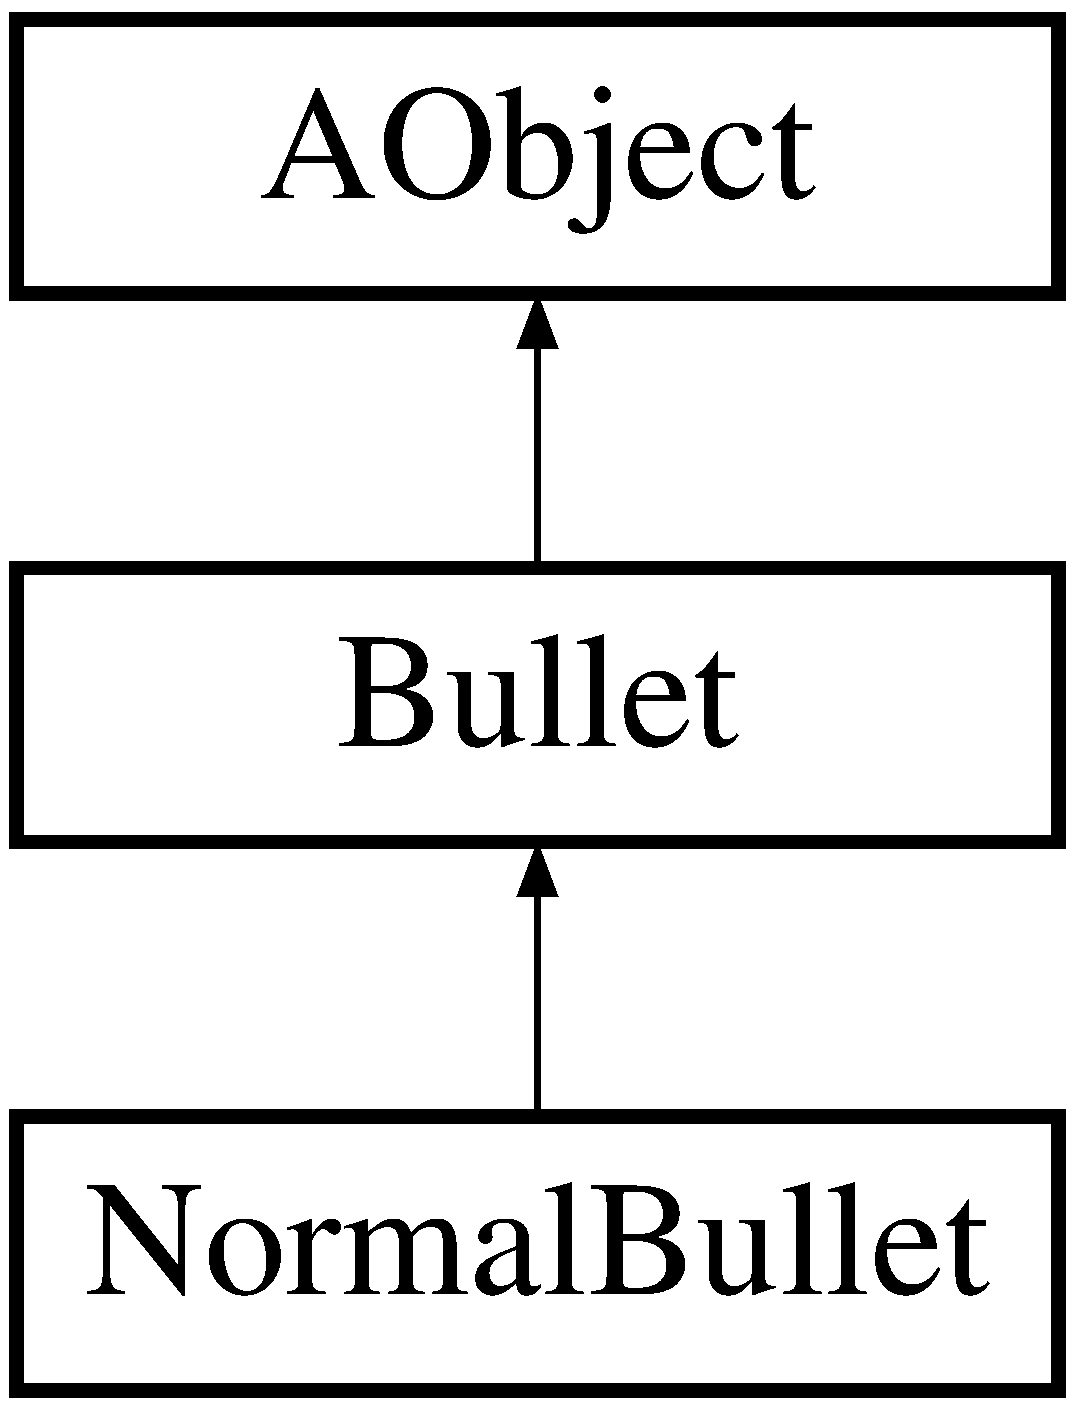
\includegraphics[height=3.000000cm]{class_normal_bullet}
\end{center}
\end{figure}
\subsection*{公開メンバ関数}
\begin{DoxyCompactItemize}
\item 
\hyperlink{class_normal_bullet_add2bcc3b93849c896f64229fde79254f}{Normal\+Bullet} (double x, double y, int \hyperlink{class_bullet_a6e5b78574ec8fbff411b1319cf111799}{damage}, int \hyperlink{class_a_object_abb924b7e558a2f9d86f2db2bc2fb18a4}{speed}, double hit\+\_\+size\+\_\+x, double hit\+\_\+size\+\_\+y, bool \hyperlink{class_a_object_a7453abe76bbddf446aa5787231428a52}{right})
\item 
void \hyperlink{class_normal_bullet_a9b45cff025d4c522b290c8c7056fae74}{Initialize} (double x, double y, bool \hyperlink{class_a_object_a7453abe76bbddf446aa5787231428a52}{right})
\item 
\hyperlink{class_normal_bullet_a3f66cb167c1499518d07e3bcb38678b6}{$\sim$\+Normal\+Bullet} (void)
\end{DoxyCompactItemize}
\subsection*{その他の継承メンバ}


\subsection{構築子と解体子}
\hypertarget{class_normal_bullet_add2bcc3b93849c896f64229fde79254f}{\index{Normal\+Bullet@{Normal\+Bullet}!Normal\+Bullet@{Normal\+Bullet}}
\index{Normal\+Bullet@{Normal\+Bullet}!Normal\+Bullet@{Normal\+Bullet}}
\subsubsection[{Normal\+Bullet}]{\setlength{\rightskip}{0pt plus 5cm}Normal\+Bullet\+::\+Normal\+Bullet (
\begin{DoxyParamCaption}
\item[{double}]{x, }
\item[{double}]{y, }
\item[{int}]{damage, }
\item[{int}]{speed, }
\item[{double}]{hit\+\_\+size\+\_\+x, }
\item[{double}]{hit\+\_\+size\+\_\+y, }
\item[{bool}]{right}
\end{DoxyParamCaption}
)}}\label{class_normal_bullet_add2bcc3b93849c896f64229fde79254f}
\hypertarget{class_normal_bullet_a3f66cb167c1499518d07e3bcb38678b6}{\index{Normal\+Bullet@{Normal\+Bullet}!````~Normal\+Bullet@{$\sim$\+Normal\+Bullet}}
\index{````~Normal\+Bullet@{$\sim$\+Normal\+Bullet}!Normal\+Bullet@{Normal\+Bullet}}
\subsubsection[{$\sim$\+Normal\+Bullet}]{\setlength{\rightskip}{0pt plus 5cm}Normal\+Bullet\+::$\sim$\+Normal\+Bullet (
\begin{DoxyParamCaption}
\item[{void}]{}
\end{DoxyParamCaption}
)}}\label{class_normal_bullet_a3f66cb167c1499518d07e3bcb38678b6}


\subsection{関数詳解}
\hypertarget{class_normal_bullet_a9b45cff025d4c522b290c8c7056fae74}{\index{Normal\+Bullet@{Normal\+Bullet}!Initialize@{Initialize}}
\index{Initialize@{Initialize}!Normal\+Bullet@{Normal\+Bullet}}
\subsubsection[{Initialize}]{\setlength{\rightskip}{0pt plus 5cm}void Normal\+Bullet\+::\+Initialize (
\begin{DoxyParamCaption}
\item[{double}]{x, }
\item[{double}]{y, }
\item[{bool}]{right}
\end{DoxyParamCaption}
)}}\label{class_normal_bullet_a9b45cff025d4c522b290c8c7056fae74}


このクラス詳解は次のファイルから抽出されました\+:\begin{DoxyCompactItemize}
\item 
\hyperlink{_normal_bullet_8h}{Normal\+Bullet.\+h}\item 
\hyperlink{_normal_bullet_8cpp}{Normal\+Bullet.\+cpp}\end{DoxyCompactItemize}

\hypertarget{class_object_manager}{\section{Object\+Manager クラス}
\label{class_object_manager}\index{Object\+Manager@{Object\+Manager}}
}


{\ttfamily \#include $<$Object\+Manager.\+h$>$}

\subsection*{公開メンバ関数}
\begin{DoxyCompactItemize}
\item 
\hyperlink{class_object_manager_a6fa9372c7c3a8da88412f4158ca3dfd9}{Object\+Manager} ()
\item 
\hyperlink{class_object_manager_a5e85ac955343ab559ece72451eaa57c1}{Object\+Manager} (int map\+\_\+width, int map\+\_\+height)
\item 
int \hyperlink{class_object_manager_afdf00874bff548b6d594d14b243241b3}{Register\+Object} (int cell\+\_\+x, int cell\+\_\+y, \hyperlink{_map_8h_ae7d76fffddf7fd7ef5d9466f971fc8e9}{Map\+Chip} map\+\_\+chip)
\item 
int \hyperlink{class_object_manager_a103f531d718ac57a39169f57d05a22cd}{Get\+Id} (int cell\+\_\+x, int cell\+\_\+y)
\item 
\hyperlink{struct_two_dimension}{Two\+Dimension} \hyperlink{class_object_manager_a89f072e56c22d2fafd15aff2c16df8dd}{Get\+Cell\+Pos\+From\+Id} (int id)
\item 
\hyperlink{class_object_manager_a25b057e6d1e60c9cbeb29d41923d8c2c}{$\sim$\+Object\+Manager} ()
\end{DoxyCompactItemize}
\subsection*{非公開変数類}
\begin{DoxyCompactItemize}
\item 
int $\ast$$\ast$ \hyperlink{class_object_manager_ae96857805143e168769f972f9b16bd09}{ids}
\item 
int \hyperlink{class_object_manager_a164a320ca3c3de4530536827d99a6458}{id\+\_\+counter}
\item 
int \hyperlink{class_object_manager_ae832dadf8bc59ae778c14c38065707aa}{width}
\item 
int \hyperlink{class_object_manager_a83650f15c75a9f0f0415966e15b2ad4f}{height}
\end{DoxyCompactItemize}


\subsection{構築子と解体子}
\hypertarget{class_object_manager_a6fa9372c7c3a8da88412f4158ca3dfd9}{\index{Object\+Manager@{Object\+Manager}!Object\+Manager@{Object\+Manager}}
\index{Object\+Manager@{Object\+Manager}!Object\+Manager@{Object\+Manager}}
\subsubsection[{Object\+Manager}]{\setlength{\rightskip}{0pt plus 5cm}Object\+Manager\+::\+Object\+Manager (
\begin{DoxyParamCaption}
{}
\end{DoxyParamCaption}
)}}\label{class_object_manager_a6fa9372c7c3a8da88412f4158ca3dfd9}
\hypertarget{class_object_manager_a5e85ac955343ab559ece72451eaa57c1}{\index{Object\+Manager@{Object\+Manager}!Object\+Manager@{Object\+Manager}}
\index{Object\+Manager@{Object\+Manager}!Object\+Manager@{Object\+Manager}}
\subsubsection[{Object\+Manager}]{\setlength{\rightskip}{0pt plus 5cm}Object\+Manager\+::\+Object\+Manager (
\begin{DoxyParamCaption}
\item[{int}]{map\+\_\+width, }
\item[{int}]{map\+\_\+height}
\end{DoxyParamCaption}
)}}\label{class_object_manager_a5e85ac955343ab559ece72451eaa57c1}
\hypertarget{class_object_manager_a25b057e6d1e60c9cbeb29d41923d8c2c}{\index{Object\+Manager@{Object\+Manager}!````~Object\+Manager@{$\sim$\+Object\+Manager}}
\index{````~Object\+Manager@{$\sim$\+Object\+Manager}!Object\+Manager@{Object\+Manager}}
\subsubsection[{$\sim$\+Object\+Manager}]{\setlength{\rightskip}{0pt plus 5cm}Object\+Manager\+::$\sim$\+Object\+Manager (
\begin{DoxyParamCaption}
{}
\end{DoxyParamCaption}
)}}\label{class_object_manager_a25b057e6d1e60c9cbeb29d41923d8c2c}


\subsection{関数詳解}
\hypertarget{class_object_manager_a89f072e56c22d2fafd15aff2c16df8dd}{\index{Object\+Manager@{Object\+Manager}!Get\+Cell\+Pos\+From\+Id@{Get\+Cell\+Pos\+From\+Id}}
\index{Get\+Cell\+Pos\+From\+Id@{Get\+Cell\+Pos\+From\+Id}!Object\+Manager@{Object\+Manager}}
\subsubsection[{Get\+Cell\+Pos\+From\+Id}]{\setlength{\rightskip}{0pt plus 5cm}{\bf Two\+Dimension} Object\+Manager\+::\+Get\+Cell\+Pos\+From\+Id (
\begin{DoxyParamCaption}
\item[{int}]{id}
\end{DoxyParamCaption}
)}}\label{class_object_manager_a89f072e56c22d2fafd15aff2c16df8dd}
\hypertarget{class_object_manager_a103f531d718ac57a39169f57d05a22cd}{\index{Object\+Manager@{Object\+Manager}!Get\+Id@{Get\+Id}}
\index{Get\+Id@{Get\+Id}!Object\+Manager@{Object\+Manager}}
\subsubsection[{Get\+Id}]{\setlength{\rightskip}{0pt plus 5cm}int Object\+Manager\+::\+Get\+Id (
\begin{DoxyParamCaption}
\item[{int}]{cell\+\_\+x, }
\item[{int}]{cell\+\_\+y}
\end{DoxyParamCaption}
)}}\label{class_object_manager_a103f531d718ac57a39169f57d05a22cd}
\hypertarget{class_object_manager_afdf00874bff548b6d594d14b243241b3}{\index{Object\+Manager@{Object\+Manager}!Register\+Object@{Register\+Object}}
\index{Register\+Object@{Register\+Object}!Object\+Manager@{Object\+Manager}}
\subsubsection[{Register\+Object}]{\setlength{\rightskip}{0pt plus 5cm}int Object\+Manager\+::\+Register\+Object (
\begin{DoxyParamCaption}
\item[{int}]{cell\+\_\+x, }
\item[{int}]{cell\+\_\+y, }
\item[{{\bf Map\+Chip}}]{map\+\_\+chip}
\end{DoxyParamCaption}
)}}\label{class_object_manager_afdf00874bff548b6d594d14b243241b3}


\subsection{メンバ詳解}
\hypertarget{class_object_manager_a83650f15c75a9f0f0415966e15b2ad4f}{\index{Object\+Manager@{Object\+Manager}!height@{height}}
\index{height@{height}!Object\+Manager@{Object\+Manager}}
\subsubsection[{height}]{\setlength{\rightskip}{0pt plus 5cm}int Object\+Manager\+::height\hspace{0.3cm}{\ttfamily [private]}}}\label{class_object_manager_a83650f15c75a9f0f0415966e15b2ad4f}
\hypertarget{class_object_manager_a164a320ca3c3de4530536827d99a6458}{\index{Object\+Manager@{Object\+Manager}!id\+\_\+counter@{id\+\_\+counter}}
\index{id\+\_\+counter@{id\+\_\+counter}!Object\+Manager@{Object\+Manager}}
\subsubsection[{id\+\_\+counter}]{\setlength{\rightskip}{0pt plus 5cm}int Object\+Manager\+::id\+\_\+counter\hspace{0.3cm}{\ttfamily [private]}}}\label{class_object_manager_a164a320ca3c3de4530536827d99a6458}
\hypertarget{class_object_manager_ae96857805143e168769f972f9b16bd09}{\index{Object\+Manager@{Object\+Manager}!ids@{ids}}
\index{ids@{ids}!Object\+Manager@{Object\+Manager}}
\subsubsection[{ids}]{\setlength{\rightskip}{0pt plus 5cm}int$\ast$$\ast$ Object\+Manager\+::ids\hspace{0.3cm}{\ttfamily [private]}}}\label{class_object_manager_ae96857805143e168769f972f9b16bd09}
\hypertarget{class_object_manager_ae832dadf8bc59ae778c14c38065707aa}{\index{Object\+Manager@{Object\+Manager}!width@{width}}
\index{width@{width}!Object\+Manager@{Object\+Manager}}
\subsubsection[{width}]{\setlength{\rightskip}{0pt plus 5cm}int Object\+Manager\+::width\hspace{0.3cm}{\ttfamily [private]}}}\label{class_object_manager_ae832dadf8bc59ae778c14c38065707aa}


このクラス詳解は次のファイルから抽出されました\+:\begin{DoxyCompactItemize}
\item 
\hyperlink{_object_manager_8h}{Object\+Manager.\+h}\item 
\hyperlink{_object_manager_8cpp}{Object\+Manager.\+cpp}\end{DoxyCompactItemize}

\hypertarget{class_player}{\section{Player クラス}
\label{class_player}\index{Player@{Player}}
}


{\ttfamily \#include $<$Player.\+h$>$}

Player の継承関係図\begin{figure}[H]
\begin{center}
\leavevmode
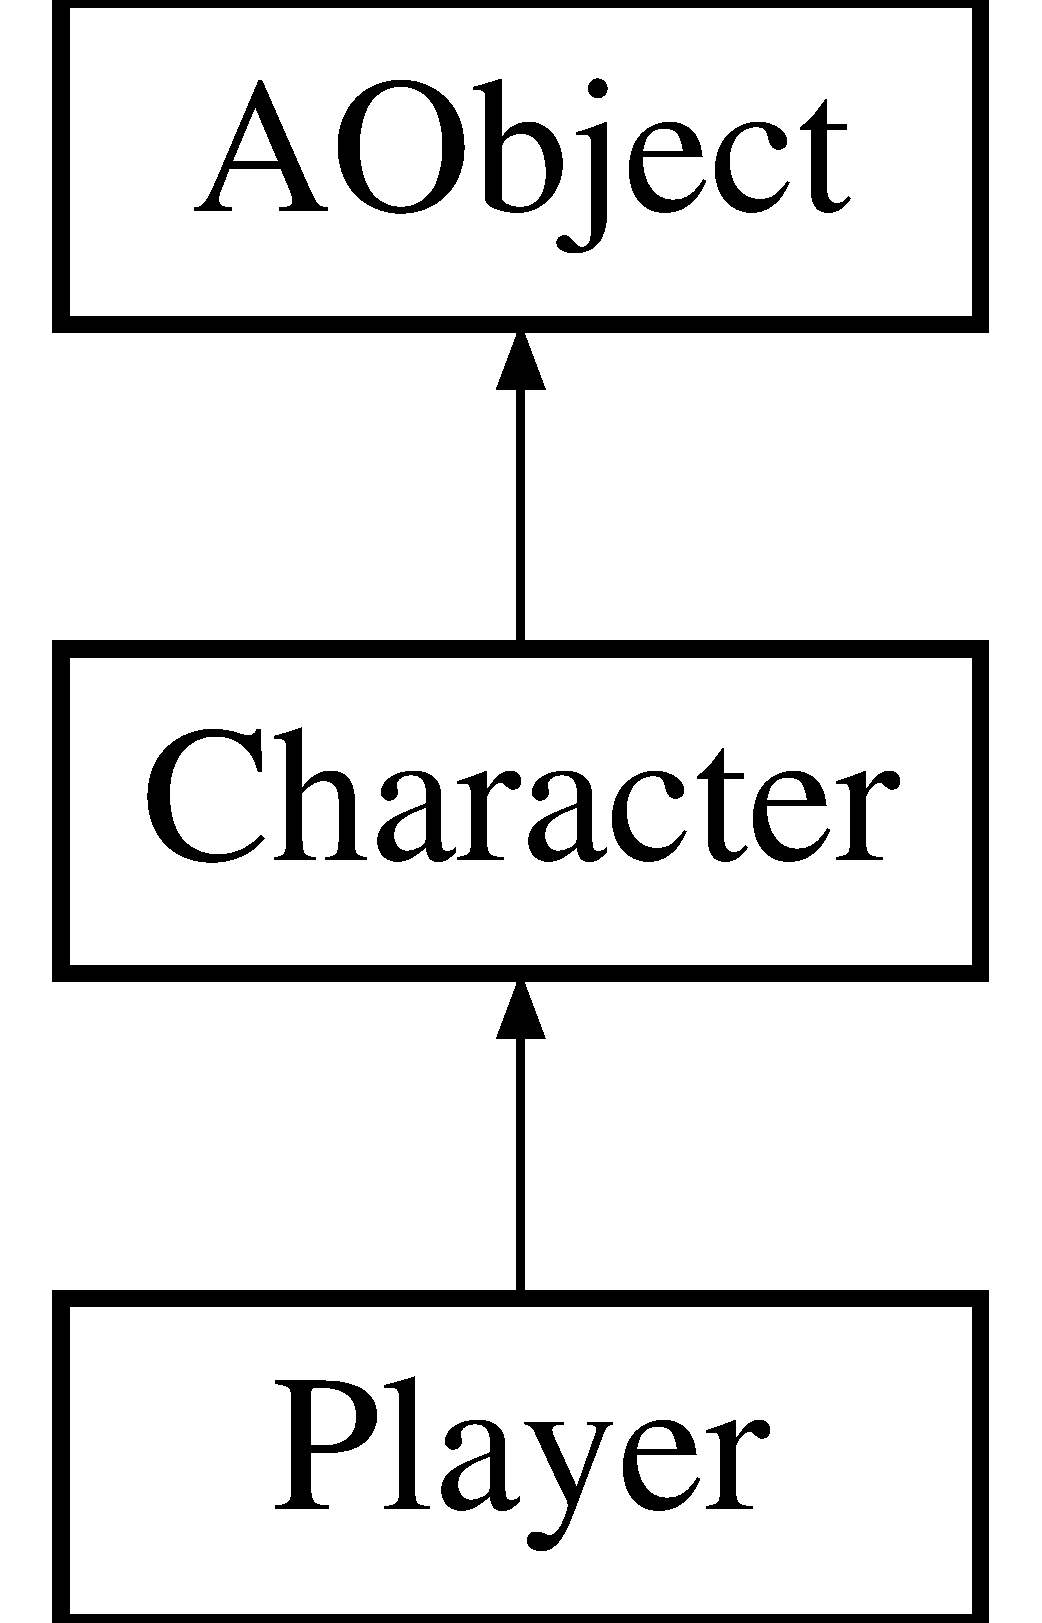
\includegraphics[height=3.000000cm]{class_player}
\end{center}
\end{figure}
\subsection*{公開メンバ関数}
\begin{DoxyCompactItemize}
\item 
\hyperlink{class_player_a03542e946924b8084cb2a8af99dc30e5}{Player} (double x, double y, \hyperlink{class_field}{Field} $\ast$field)
\item 
void \hyperlink{class_player_abc93f150c044405d86ebfceb5026b546}{add\+Score} (int point)
\item 
void \hyperlink{class_player_a8fa34b8279dd879ad2b56d3ed77e4963}{Change\+Clear} ()
\item 
void \hyperlink{class_player_a33b2feb64c47c415d4ce2709bac934cc}{Set\+Game\+Status} (\hyperlink{_player_8h_a3f619558ea4f7947c437250166fbd29b}{G\+A\+M\+E\+\_\+\+S\+T\+A\+T\+U\+S} \hyperlink{class_player_a6eaebcae8a2d8e90033ba21ed3065b91}{game\+\_\+status})
\item 
void \hyperlink{class_player_a2e85dba0b04af54c87dd2819b637512b}{super\+Time} ()
\item 
int \hyperlink{class_player_a0b5af9f507f7901efcc8ab8ee85e02a5}{score} ()
\item 
int \hyperlink{class_player_a012e5b3b06efa727a230b0b4d44eeafd}{life} ()
\item 
bool \hyperlink{class_player_abaf0c48bc8bd4a1f04d45821cebc17ea}{super} ()
\item 
int \hyperlink{class_player_ac8f40782910567cac2a45bc12bd668b5}{super\+Count} ()
\item 
bool \hyperlink{class_player_aa620c2ad442cf120fab24bee89006050}{Is\+Clear} ()
\item 
\hyperlink{_player_8h_a3f619558ea4f7947c437250166fbd29b}{G\+A\+M\+E\+\_\+\+S\+T\+A\+T\+U\+S} \hyperlink{class_player_a6eaebcae8a2d8e90033ba21ed3065b91}{game\+\_\+status} ()
\item 
void \hyperlink{class_player_a1334990b8b7aaaad904e22f03f4d947d}{Jump} ()
\item 
void \hyperlink{class_player_ab60f92a8070d5522ffaf30dbc8224a36}{Damaged} (int damage)
\item 
void \hyperlink{class_player_a22a0d2b901622c497b677b7c75fafe45}{Reset} ()
\item 
void \hyperlink{class_player_a5e32dec9258cfa8145e482fed4c42c83}{Draw} (int offset)
\end{DoxyCompactItemize}
\subsection*{非公開変数類}
\begin{DoxyCompactItemize}
\item 
int \hyperlink{class_player_a3ffa2ba8dfce8924e4b2b2cae65e2831}{life\+\_\+}
\item 
int \hyperlink{class_player_a423e2096b25d4965a84e4a8bf38c7683}{score\+\_\+}
\item 
bool \hyperlink{class_player_a36ffd35693d223b63089517cc059f98a}{super\+\_\+}
\item 
int \hyperlink{class_player_a141db66821f18e72907efd017533603f}{super\+\_\+count\+\_\+}
\item 
bool \hyperlink{class_player_a186aacf08edf0bd9eb3d3ade1c012409}{clear}
\item 
\hyperlink{_player_8h_a3f619558ea4f7947c437250166fbd29b}{G\+A\+M\+E\+\_\+\+S\+T\+A\+T\+U\+S} \hyperlink{class_player_adcdab78aadb61281eb3346e32c103192}{game\+\_\+status\+\_\+}
\end{DoxyCompactItemize}
\subsection*{その他の継承メンバ}


\subsection{構築子と解体子}
\hypertarget{class_player_a03542e946924b8084cb2a8af99dc30e5}{\index{Player@{Player}!Player@{Player}}
\index{Player@{Player}!Player@{Player}}
\subsubsection[{Player}]{\setlength{\rightskip}{0pt plus 5cm}Player\+::\+Player (
\begin{DoxyParamCaption}
\item[{double}]{x, }
\item[{double}]{y, }
\item[{{\bf Field} $\ast$}]{field}
\end{DoxyParamCaption}
)}}\label{class_player_a03542e946924b8084cb2a8af99dc30e5}


\subsection{関数詳解}
\hypertarget{class_player_abc93f150c044405d86ebfceb5026b546}{\index{Player@{Player}!add\+Score@{add\+Score}}
\index{add\+Score@{add\+Score}!Player@{Player}}
\subsubsection[{add\+Score}]{\setlength{\rightskip}{0pt plus 5cm}void Player\+::add\+Score (
\begin{DoxyParamCaption}
\item[{int}]{point}
\end{DoxyParamCaption}
)}}\label{class_player_abc93f150c044405d86ebfceb5026b546}
\hypertarget{class_player_a8fa34b8279dd879ad2b56d3ed77e4963}{\index{Player@{Player}!Change\+Clear@{Change\+Clear}}
\index{Change\+Clear@{Change\+Clear}!Player@{Player}}
\subsubsection[{Change\+Clear}]{\setlength{\rightskip}{0pt plus 5cm}void Player\+::\+Change\+Clear (
\begin{DoxyParamCaption}
{}
\end{DoxyParamCaption}
)\hspace{0.3cm}{\ttfamily [inline]}}}\label{class_player_a8fa34b8279dd879ad2b56d3ed77e4963}
\hypertarget{class_player_ab60f92a8070d5522ffaf30dbc8224a36}{\index{Player@{Player}!Damaged@{Damaged}}
\index{Damaged@{Damaged}!Player@{Player}}
\subsubsection[{Damaged}]{\setlength{\rightskip}{0pt plus 5cm}void Player\+::\+Damaged (
\begin{DoxyParamCaption}
\item[{int}]{damage}
\end{DoxyParamCaption}
)}}\label{class_player_ab60f92a8070d5522ffaf30dbc8224a36}
\hypertarget{class_player_a5e32dec9258cfa8145e482fed4c42c83}{\index{Player@{Player}!Draw@{Draw}}
\index{Draw@{Draw}!Player@{Player}}
\subsubsection[{Draw}]{\setlength{\rightskip}{0pt plus 5cm}void Player\+::\+Draw (
\begin{DoxyParamCaption}
\item[{int}]{offset}
\end{DoxyParamCaption}
)\hspace{0.3cm}{\ttfamily [virtual]}}}\label{class_player_a5e32dec9258cfa8145e482fed4c42c83}


\hyperlink{class_character_ad359a991510783008ee96060f247c990}{Character}を再実装しています。

\hypertarget{class_player_a6eaebcae8a2d8e90033ba21ed3065b91}{\index{Player@{Player}!game\+\_\+status@{game\+\_\+status}}
\index{game\+\_\+status@{game\+\_\+status}!Player@{Player}}
\subsubsection[{game\+\_\+status}]{\setlength{\rightskip}{0pt plus 5cm}{\bf G\+A\+M\+E\+\_\+\+S\+T\+A\+T\+U\+S} Player\+::game\+\_\+status (
\begin{DoxyParamCaption}
{}
\end{DoxyParamCaption}
)\hspace{0.3cm}{\ttfamily [inline]}}}\label{class_player_a6eaebcae8a2d8e90033ba21ed3065b91}
\hypertarget{class_player_aa620c2ad442cf120fab24bee89006050}{\index{Player@{Player}!Is\+Clear@{Is\+Clear}}
\index{Is\+Clear@{Is\+Clear}!Player@{Player}}
\subsubsection[{Is\+Clear}]{\setlength{\rightskip}{0pt plus 5cm}bool Player\+::\+Is\+Clear (
\begin{DoxyParamCaption}
{}
\end{DoxyParamCaption}
)\hspace{0.3cm}{\ttfamily [inline]}}}\label{class_player_aa620c2ad442cf120fab24bee89006050}
\hypertarget{class_player_a1334990b8b7aaaad904e22f03f4d947d}{\index{Player@{Player}!Jump@{Jump}}
\index{Jump@{Jump}!Player@{Player}}
\subsubsection[{Jump}]{\setlength{\rightskip}{0pt plus 5cm}void Player\+::\+Jump (
\begin{DoxyParamCaption}
{}
\end{DoxyParamCaption}
)\hspace{0.3cm}{\ttfamily [virtual]}}}\label{class_player_a1334990b8b7aaaad904e22f03f4d947d}


\hyperlink{class_character_a7622bdde334c8d37358218e64dd6850a}{Character}を再実装しています。

\hypertarget{class_player_a012e5b3b06efa727a230b0b4d44eeafd}{\index{Player@{Player}!life@{life}}
\index{life@{life}!Player@{Player}}
\subsubsection[{life}]{\setlength{\rightskip}{0pt plus 5cm}int Player\+::life (
\begin{DoxyParamCaption}
{}
\end{DoxyParamCaption}
)\hspace{0.3cm}{\ttfamily [inline]}}}\label{class_player_a012e5b3b06efa727a230b0b4d44eeafd}
\hypertarget{class_player_a22a0d2b901622c497b677b7c75fafe45}{\index{Player@{Player}!Reset@{Reset}}
\index{Reset@{Reset}!Player@{Player}}
\subsubsection[{Reset}]{\setlength{\rightskip}{0pt plus 5cm}void Player\+::\+Reset (
\begin{DoxyParamCaption}
{}
\end{DoxyParamCaption}
)\hspace{0.3cm}{\ttfamily [virtual]}}}\label{class_player_a22a0d2b901622c497b677b7c75fafe45}


\hyperlink{class_character_a6c1fa20d22b5ea6edc4dbd6ca9496411}{Character}を再実装しています。

\hypertarget{class_player_a0b5af9f507f7901efcc8ab8ee85e02a5}{\index{Player@{Player}!score@{score}}
\index{score@{score}!Player@{Player}}
\subsubsection[{score}]{\setlength{\rightskip}{0pt plus 5cm}int Player\+::score (
\begin{DoxyParamCaption}
{}
\end{DoxyParamCaption}
)\hspace{0.3cm}{\ttfamily [inline]}}}\label{class_player_a0b5af9f507f7901efcc8ab8ee85e02a5}
\hypertarget{class_player_a33b2feb64c47c415d4ce2709bac934cc}{\index{Player@{Player}!Set\+Game\+Status@{Set\+Game\+Status}}
\index{Set\+Game\+Status@{Set\+Game\+Status}!Player@{Player}}
\subsubsection[{Set\+Game\+Status}]{\setlength{\rightskip}{0pt plus 5cm}void Player\+::\+Set\+Game\+Status (
\begin{DoxyParamCaption}
\item[{{\bf G\+A\+M\+E\+\_\+\+S\+T\+A\+T\+U\+S}}]{game\+\_\+status}
\end{DoxyParamCaption}
)\hspace{0.3cm}{\ttfamily [inline]}}}\label{class_player_a33b2feb64c47c415d4ce2709bac934cc}
\hypertarget{class_player_abaf0c48bc8bd4a1f04d45821cebc17ea}{\index{Player@{Player}!super@{super}}
\index{super@{super}!Player@{Player}}
\subsubsection[{super}]{\setlength{\rightskip}{0pt plus 5cm}bool Player\+::super (
\begin{DoxyParamCaption}
{}
\end{DoxyParamCaption}
)\hspace{0.3cm}{\ttfamily [inline]}}}\label{class_player_abaf0c48bc8bd4a1f04d45821cebc17ea}
\hypertarget{class_player_ac8f40782910567cac2a45bc12bd668b5}{\index{Player@{Player}!super\+Count@{super\+Count}}
\index{super\+Count@{super\+Count}!Player@{Player}}
\subsubsection[{super\+Count}]{\setlength{\rightskip}{0pt plus 5cm}int Player\+::super\+Count (
\begin{DoxyParamCaption}
{}
\end{DoxyParamCaption}
)\hspace{0.3cm}{\ttfamily [inline]}}}\label{class_player_ac8f40782910567cac2a45bc12bd668b5}
\hypertarget{class_player_a2e85dba0b04af54c87dd2819b637512b}{\index{Player@{Player}!super\+Time@{super\+Time}}
\index{super\+Time@{super\+Time}!Player@{Player}}
\subsubsection[{super\+Time}]{\setlength{\rightskip}{0pt plus 5cm}void Player\+::super\+Time (
\begin{DoxyParamCaption}
{}
\end{DoxyParamCaption}
)}}\label{class_player_a2e85dba0b04af54c87dd2819b637512b}


\subsection{メンバ詳解}
\hypertarget{class_player_a186aacf08edf0bd9eb3d3ade1c012409}{\index{Player@{Player}!clear@{clear}}
\index{clear@{clear}!Player@{Player}}
\subsubsection[{clear}]{\setlength{\rightskip}{0pt plus 5cm}bool Player\+::clear\hspace{0.3cm}{\ttfamily [private]}}}\label{class_player_a186aacf08edf0bd9eb3d3ade1c012409}
\hypertarget{class_player_adcdab78aadb61281eb3346e32c103192}{\index{Player@{Player}!game\+\_\+status\+\_\+@{game\+\_\+status\+\_\+}}
\index{game\+\_\+status\+\_\+@{game\+\_\+status\+\_\+}!Player@{Player}}
\subsubsection[{game\+\_\+status\+\_\+}]{\setlength{\rightskip}{0pt plus 5cm}{\bf G\+A\+M\+E\+\_\+\+S\+T\+A\+T\+U\+S} Player\+::game\+\_\+status\+\_\+\hspace{0.3cm}{\ttfamily [private]}}}\label{class_player_adcdab78aadb61281eb3346e32c103192}
\hypertarget{class_player_a3ffa2ba8dfce8924e4b2b2cae65e2831}{\index{Player@{Player}!life\+\_\+@{life\+\_\+}}
\index{life\+\_\+@{life\+\_\+}!Player@{Player}}
\subsubsection[{life\+\_\+}]{\setlength{\rightskip}{0pt plus 5cm}int Player\+::life\+\_\+\hspace{0.3cm}{\ttfamily [private]}}}\label{class_player_a3ffa2ba8dfce8924e4b2b2cae65e2831}
\hypertarget{class_player_a423e2096b25d4965a84e4a8bf38c7683}{\index{Player@{Player}!score\+\_\+@{score\+\_\+}}
\index{score\+\_\+@{score\+\_\+}!Player@{Player}}
\subsubsection[{score\+\_\+}]{\setlength{\rightskip}{0pt plus 5cm}int Player\+::score\+\_\+\hspace{0.3cm}{\ttfamily [private]}}}\label{class_player_a423e2096b25d4965a84e4a8bf38c7683}
\hypertarget{class_player_a36ffd35693d223b63089517cc059f98a}{\index{Player@{Player}!super\+\_\+@{super\+\_\+}}
\index{super\+\_\+@{super\+\_\+}!Player@{Player}}
\subsubsection[{super\+\_\+}]{\setlength{\rightskip}{0pt plus 5cm}bool Player\+::super\+\_\+\hspace{0.3cm}{\ttfamily [private]}}}\label{class_player_a36ffd35693d223b63089517cc059f98a}
\hypertarget{class_player_a141db66821f18e72907efd017533603f}{\index{Player@{Player}!super\+\_\+count\+\_\+@{super\+\_\+count\+\_\+}}
\index{super\+\_\+count\+\_\+@{super\+\_\+count\+\_\+}!Player@{Player}}
\subsubsection[{super\+\_\+count\+\_\+}]{\setlength{\rightskip}{0pt plus 5cm}int Player\+::super\+\_\+count\+\_\+\hspace{0.3cm}{\ttfamily [private]}}}\label{class_player_a141db66821f18e72907efd017533603f}


このクラス詳解は次のファイルから抽出されました\+:\begin{DoxyCompactItemize}
\item 
\hyperlink{_player_8h}{Player.\+h}\item 
\hyperlink{_player_8cpp}{Player.\+cpp}\end{DoxyCompactItemize}

\hypertarget{class_player_controller}{\section{Player\+Controller クラス}
\label{class_player_controller}\index{Player\+Controller@{Player\+Controller}}
}


{\ttfamily \#include $<$Player\+Controller.\+h$>$}

Player\+Controller の継承関係図\begin{figure}[H]
\begin{center}
\leavevmode
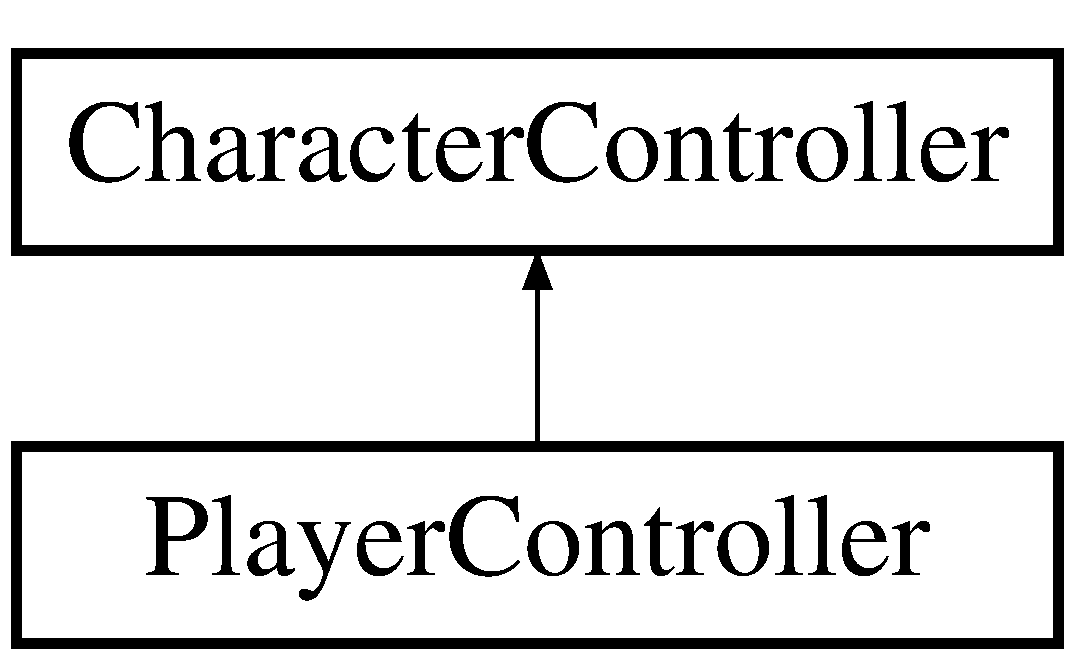
\includegraphics[height=2.000000cm]{class_player_controller}
\end{center}
\end{figure}
\subsection*{公開メンバ関数}
\begin{DoxyCompactItemize}
\item 
\hyperlink{class_player_controller_af2d4e93f407c9cd40a5de9f14cbeadec}{Player\+Controller} ()
\item 
\hyperlink{class_player_controller_a8becc11a59c07bf97ddac1a81771837b}{Player\+Controller} (\hyperlink{class_character}{Character} $\ast$character, \hyperlink{class_field}{Field} $\ast$field)
\item 
void \hyperlink{class_player_controller_a3331f219d6f6a735c1e6cda5e8abb298}{Think} ()
\end{DoxyCompactItemize}
\subsection*{非公開メンバ関数}
\begin{DoxyCompactItemize}
\item 
void \hyperlink{class_player_controller_ac0a4cf90b4d133b4279633fb6c692979}{Update\+Key} ()
\end{DoxyCompactItemize}
\subsection*{非公開変数類}
\begin{DoxyCompactItemize}
\item 
char \hyperlink{class_player_controller_adc832677d282a6a701478e1eada10053}{key} \mbox{[}256\mbox{]}
\end{DoxyCompactItemize}
\subsection*{その他の継承メンバ}


\subsection{構築子と解体子}
\hypertarget{class_player_controller_af2d4e93f407c9cd40a5de9f14cbeadec}{\index{Player\+Controller@{Player\+Controller}!Player\+Controller@{Player\+Controller}}
\index{Player\+Controller@{Player\+Controller}!Player\+Controller@{Player\+Controller}}
\subsubsection[{Player\+Controller}]{\setlength{\rightskip}{0pt plus 5cm}Player\+Controller\+::\+Player\+Controller (
\begin{DoxyParamCaption}
{}
\end{DoxyParamCaption}
)}}\label{class_player_controller_af2d4e93f407c9cd40a5de9f14cbeadec}
\hypertarget{class_player_controller_a8becc11a59c07bf97ddac1a81771837b}{\index{Player\+Controller@{Player\+Controller}!Player\+Controller@{Player\+Controller}}
\index{Player\+Controller@{Player\+Controller}!Player\+Controller@{Player\+Controller}}
\subsubsection[{Player\+Controller}]{\setlength{\rightskip}{0pt plus 5cm}Player\+Controller\+::\+Player\+Controller (
\begin{DoxyParamCaption}
\item[{{\bf Character} $\ast$}]{character, }
\item[{{\bf Field} $\ast$}]{field}
\end{DoxyParamCaption}
)}}\label{class_player_controller_a8becc11a59c07bf97ddac1a81771837b}


\subsection{関数詳解}
\hypertarget{class_player_controller_a3331f219d6f6a735c1e6cda5e8abb298}{\index{Player\+Controller@{Player\+Controller}!Think@{Think}}
\index{Think@{Think}!Player\+Controller@{Player\+Controller}}
\subsubsection[{Think}]{\setlength{\rightskip}{0pt plus 5cm}void Player\+Controller\+::\+Think (
\begin{DoxyParamCaption}
{}
\end{DoxyParamCaption}
)\hspace{0.3cm}{\ttfamily [virtual]}}}\label{class_player_controller_a3331f219d6f6a735c1e6cda5e8abb298}


\hyperlink{class_character_controller_a493d5b59610546133900f4de7110a487}{Character\+Controller}を実装しています。

\hypertarget{class_player_controller_ac0a4cf90b4d133b4279633fb6c692979}{\index{Player\+Controller@{Player\+Controller}!Update\+Key@{Update\+Key}}
\index{Update\+Key@{Update\+Key}!Player\+Controller@{Player\+Controller}}
\subsubsection[{Update\+Key}]{\setlength{\rightskip}{0pt plus 5cm}void Player\+Controller\+::\+Update\+Key (
\begin{DoxyParamCaption}
{}
\end{DoxyParamCaption}
)\hspace{0.3cm}{\ttfamily [private]}}}\label{class_player_controller_ac0a4cf90b4d133b4279633fb6c692979}


\subsection{メンバ詳解}
\hypertarget{class_player_controller_adc832677d282a6a701478e1eada10053}{\index{Player\+Controller@{Player\+Controller}!key@{key}}
\index{key@{key}!Player\+Controller@{Player\+Controller}}
\subsubsection[{key}]{\setlength{\rightskip}{0pt plus 5cm}char Player\+Controller\+::key\mbox{[}256\mbox{]}\hspace{0.3cm}{\ttfamily [private]}}}\label{class_player_controller_adc832677d282a6a701478e1eada10053}


このクラス詳解は次のファイルから抽出されました\+:\begin{DoxyCompactItemize}
\item 
\hyperlink{_player_controller_8h}{Player\+Controller.\+h}\item 
\hyperlink{_player_controller_8cpp}{Player\+Controller.\+cpp}\end{DoxyCompactItemize}

\hypertarget{struct_two_dimension}{\section{Two\+Dimension 構造体}
\label{struct_two_dimension}\index{Two\+Dimension@{Two\+Dimension}}
}


{\ttfamily \#include $<$A\+Object.\+h$>$}

\subsection*{公開変数類}
\begin{DoxyCompactItemize}
\item 
double \hyperlink{struct_two_dimension_ac7506c70d1af8d3706ed1f084a1587fb}{x}
\item 
double \hyperlink{struct_two_dimension_aa344dbcbece346bdcb1949249b4c6cfc}{y}
\end{DoxyCompactItemize}


\subsection{メンバ詳解}
\hypertarget{struct_two_dimension_ac7506c70d1af8d3706ed1f084a1587fb}{\index{Two\+Dimension@{Two\+Dimension}!x@{x}}
\index{x@{x}!Two\+Dimension@{Two\+Dimension}}
\subsubsection[{x}]{\setlength{\rightskip}{0pt plus 5cm}double Two\+Dimension\+::x}}\label{struct_two_dimension_ac7506c70d1af8d3706ed1f084a1587fb}
\hypertarget{struct_two_dimension_aa344dbcbece346bdcb1949249b4c6cfc}{\index{Two\+Dimension@{Two\+Dimension}!y@{y}}
\index{y@{y}!Two\+Dimension@{Two\+Dimension}}
\subsubsection[{y}]{\setlength{\rightskip}{0pt plus 5cm}double Two\+Dimension\+::y}}\label{struct_two_dimension_aa344dbcbece346bdcb1949249b4c6cfc}


この構造体詳解は次のファイルから抽出されました\+:\begin{DoxyCompactItemize}
\item 
\hyperlink{_a_object_8h}{A\+Object.\+h}\end{DoxyCompactItemize}

\hypertarget{class_walk_straight}{\section{Walk\+Straight クラス}
\label{class_walk_straight}\index{Walk\+Straight@{Walk\+Straight}}
}


{\ttfamily \#include $<$Walk\+Straight.\+h$>$}

Walk\+Straight の継承関係図\begin{figure}[H]
\begin{center}
\leavevmode
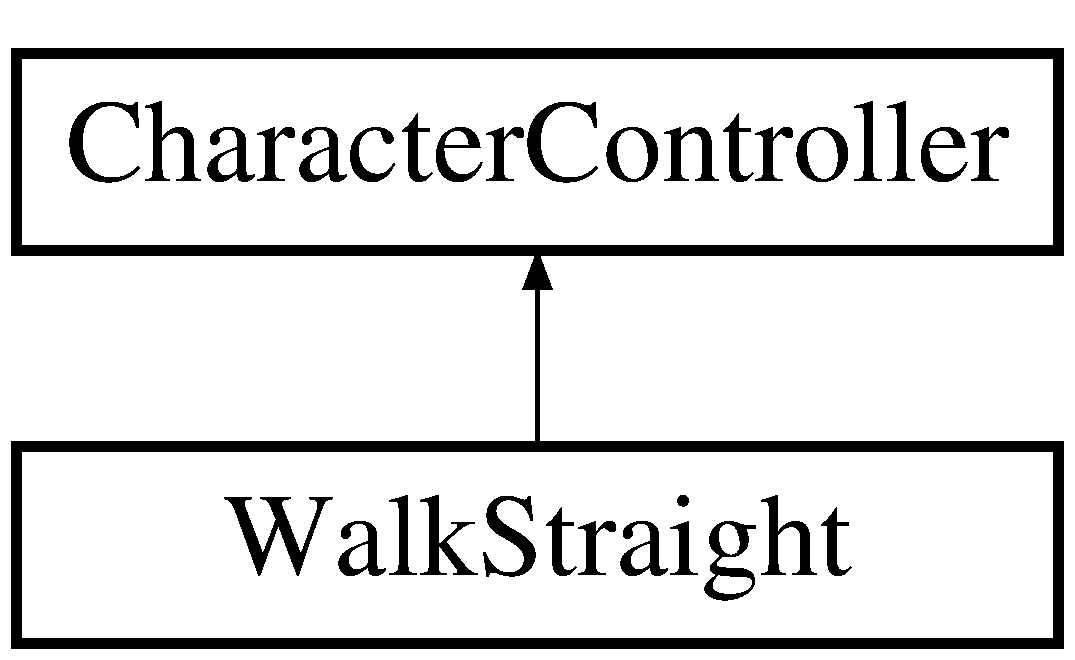
\includegraphics[height=2.000000cm]{class_walk_straight}
\end{center}
\end{figure}
\subsection*{公開メンバ関数}
\begin{DoxyCompactItemize}
\item 
\hyperlink{class_walk_straight_afe18d9357038b8bdb51fa79dcd522344}{Walk\+Straight} ()
\item 
\hyperlink{class_walk_straight_af47c11a0b42e6bf44edb2b4b7dc39591}{Walk\+Straight} (\hyperlink{class_character}{Character} $\ast$character, \hyperlink{class_field}{Field} $\ast$field)
\item 
void \hyperlink{class_walk_straight_ad8a6f6a0947df875c253752f72e9af0f}{Think} ()
\end{DoxyCompactItemize}
\subsection*{その他の継承メンバ}


\subsection{構築子と解体子}
\hypertarget{class_walk_straight_afe18d9357038b8bdb51fa79dcd522344}{\index{Walk\+Straight@{Walk\+Straight}!Walk\+Straight@{Walk\+Straight}}
\index{Walk\+Straight@{Walk\+Straight}!Walk\+Straight@{Walk\+Straight}}
\subsubsection[{Walk\+Straight}]{\setlength{\rightskip}{0pt plus 5cm}Walk\+Straight\+::\+Walk\+Straight (
\begin{DoxyParamCaption}
{}
\end{DoxyParamCaption}
)}}\label{class_walk_straight_afe18d9357038b8bdb51fa79dcd522344}
\hypertarget{class_walk_straight_af47c11a0b42e6bf44edb2b4b7dc39591}{\index{Walk\+Straight@{Walk\+Straight}!Walk\+Straight@{Walk\+Straight}}
\index{Walk\+Straight@{Walk\+Straight}!Walk\+Straight@{Walk\+Straight}}
\subsubsection[{Walk\+Straight}]{\setlength{\rightskip}{0pt plus 5cm}Walk\+Straight\+::\+Walk\+Straight (
\begin{DoxyParamCaption}
\item[{{\bf Character} $\ast$}]{character, }
\item[{{\bf Field} $\ast$}]{field}
\end{DoxyParamCaption}
)}}\label{class_walk_straight_af47c11a0b42e6bf44edb2b4b7dc39591}


\subsection{関数詳解}
\hypertarget{class_walk_straight_ad8a6f6a0947df875c253752f72e9af0f}{\index{Walk\+Straight@{Walk\+Straight}!Think@{Think}}
\index{Think@{Think}!Walk\+Straight@{Walk\+Straight}}
\subsubsection[{Think}]{\setlength{\rightskip}{0pt plus 5cm}void Walk\+Straight\+::\+Think (
\begin{DoxyParamCaption}
{}
\end{DoxyParamCaption}
)\hspace{0.3cm}{\ttfamily [virtual]}}}\label{class_walk_straight_ad8a6f6a0947df875c253752f72e9af0f}


\hyperlink{class_character_controller_a493d5b59610546133900f4de7110a487}{Character\+Controller}を実装しています。



このクラス詳解は次のファイルから抽出されました\+:\begin{DoxyCompactItemize}
\item 
\hyperlink{_walk_straight_8h}{Walk\+Straight.\+h}\item 
\hyperlink{_walk_straight_8cpp}{Walk\+Straight.\+cpp}\end{DoxyCompactItemize}

\chapter{ファイル詳解}
\hypertarget{_aim_attack_8cpp}{\section{Aim\+Attack.\+cpp ファイル}
\label{_aim_attack_8cpp}\index{Aim\+Attack.\+cpp@{Aim\+Attack.\+cpp}}
}
{\ttfamily \#include \char`\"{}Aim\+Attack.\+h\char`\"{}}\\*

\hypertarget{_aim_attack_8h}{\section{Aim\+Attack.\+h ファイル}
\label{_aim_attack_8h}\index{Aim\+Attack.\+h@{Aim\+Attack.\+h}}
}
{\ttfamily \#include \char`\"{}attack.\+h\char`\"{}}\\*
{\ttfamily \#include \char`\"{}Aim\+Bullet.\+h\char`\"{}}\\*
{\ttfamily \#include \char`\"{}Character.\+h\char`\"{}}\\*
\subsection*{クラス}
\begin{DoxyCompactItemize}
\item 
class \hyperlink{class_aim_attack}{Aim\+Attack}
\end{DoxyCompactItemize}

\hypertarget{_aim_bullet_8cpp}{\section{Aim\+Bullet.\+cpp ファイル}
\label{_aim_bullet_8cpp}\index{Aim\+Bullet.\+cpp@{Aim\+Bullet.\+cpp}}
}
{\ttfamily \#include \char`\"{}Aim\+Bullet.\+h\char`\"{}}\\*

\hypertarget{_aim_bullet_8h}{\section{Aim\+Bullet.\+h ファイル}
\label{_aim_bullet_8h}\index{Aim\+Bullet.\+h@{Aim\+Bullet.\+h}}
}
{\ttfamily \#include \char`\"{}bullet.\+h\char`\"{}}\\*
\subsection*{クラス}
\begin{DoxyCompactItemize}
\item 
class \hyperlink{class_aim_bullet}{Aim\+Bullet}
\end{DoxyCompactItemize}

\hypertarget{_a_object_8cpp}{\section{A\+Object.\+cpp ファイル}
\label{_a_object_8cpp}\index{A\+Object.\+cpp@{A\+Object.\+cpp}}
}
{\ttfamily \#include $<$string.\+h$>$}\\*
{\ttfamily \#include \char`\"{}A\+Object.\+h\char`\"{}}\\*

\hypertarget{_a_object_8h}{\section{A\+Object.\+h ファイル}
\label{_a_object_8h}\index{A\+Object.\+h@{A\+Object.\+h}}
}
{\ttfamily \#include \char`\"{}Dx\+Lib.\+h\char`\"{}}\\*
{\ttfamily \#include \char`\"{}Load\+Graphic.\+h\char`\"{}}\\*
\subsection*{クラス}
\begin{DoxyCompactItemize}
\item 
struct \hyperlink{struct_two_dimension}{Two\+Dimension}
\item 
class \hyperlink{class_a_object}{A\+Object}
\end{DoxyCompactItemize}
\subsection*{列挙型}
\begin{DoxyCompactItemize}
\item 
enum \hyperlink{_a_object_8h_a842c5e2e69277690b064bf363c017980}{Object\+Type} \{ \hyperlink{_a_object_8h_a842c5e2e69277690b064bf363c017980aacac6199bbab8a77e3192a8559724d8f}{O\+\_\+\+P\+L\+A\+Y\+E\+R}, 
\hyperlink{_a_object_8h_a842c5e2e69277690b064bf363c017980ab985f61c895aee454d26484d6fe712a8}{O\+\_\+\+E\+N\+E\+M\+Y}, 
\hyperlink{_a_object_8h_a842c5e2e69277690b064bf363c017980abba9a36b65eb4d21d078a078c055d9a7}{O\+\_\+\+I\+T\+E\+M}
 \}
\end{DoxyCompactItemize}


\subsection{列挙型詳解}
\hypertarget{_a_object_8h_a842c5e2e69277690b064bf363c017980}{\index{A\+Object.\+h@{A\+Object.\+h}!Object\+Type@{Object\+Type}}
\index{Object\+Type@{Object\+Type}!A\+Object.\+h@{A\+Object.\+h}}
\subsubsection[{Object\+Type}]{\setlength{\rightskip}{0pt plus 5cm}enum {\bf Object\+Type}}}\label{_a_object_8h_a842c5e2e69277690b064bf363c017980}
\begin{Desc}
\item[列挙値]\par
\begin{description}
\index{O\+\_\+\+P\+L\+A\+Y\+E\+R@{O\+\_\+\+P\+L\+A\+Y\+E\+R}!A\+Object.\+h@{A\+Object.\+h}}\index{A\+Object.\+h@{A\+Object.\+h}!O\+\_\+\+P\+L\+A\+Y\+E\+R@{O\+\_\+\+P\+L\+A\+Y\+E\+R}}\item[{\em 
\hypertarget{_a_object_8h_a842c5e2e69277690b064bf363c017980aacac6199bbab8a77e3192a8559724d8f}{O\+\_\+\+P\+L\+A\+Y\+E\+R}\label{_a_object_8h_a842c5e2e69277690b064bf363c017980aacac6199bbab8a77e3192a8559724d8f}
}]\index{O\+\_\+\+E\+N\+E\+M\+Y@{O\+\_\+\+E\+N\+E\+M\+Y}!A\+Object.\+h@{A\+Object.\+h}}\index{A\+Object.\+h@{A\+Object.\+h}!O\+\_\+\+E\+N\+E\+M\+Y@{O\+\_\+\+E\+N\+E\+M\+Y}}\item[{\em 
\hypertarget{_a_object_8h_a842c5e2e69277690b064bf363c017980ab985f61c895aee454d26484d6fe712a8}{O\+\_\+\+E\+N\+E\+M\+Y}\label{_a_object_8h_a842c5e2e69277690b064bf363c017980ab985f61c895aee454d26484d6fe712a8}
}]\index{O\+\_\+\+I\+T\+E\+M@{O\+\_\+\+I\+T\+E\+M}!A\+Object.\+h@{A\+Object.\+h}}\index{A\+Object.\+h@{A\+Object.\+h}!O\+\_\+\+I\+T\+E\+M@{O\+\_\+\+I\+T\+E\+M}}\item[{\em 
\hypertarget{_a_object_8h_a842c5e2e69277690b064bf363c017980abba9a36b65eb4d21d078a078c055d9a7}{O\+\_\+\+I\+T\+E\+M}\label{_a_object_8h_a842c5e2e69277690b064bf363c017980abba9a36b65eb4d21d078a078c055d9a7}
}]\end{description}
\end{Desc}

\hypertarget{_attack_8cpp}{\section{Attack.\+cpp ファイル}
\label{_attack_8cpp}\index{Attack.\+cpp@{Attack.\+cpp}}
}
{\ttfamily \#include \char`\"{}Attack.\+h\char`\"{}}\\*
{\ttfamily \#include \char`\"{}Character.\+h\char`\"{}}\\*

\hypertarget{_attack_8h}{\section{Attack.\+h ファイル}
\label{_attack_8h}\index{Attack.\+h@{Attack.\+h}}
}
{\ttfamily \#include \char`\"{}Bullet.\+h\char`\"{}}\\*
{\ttfamily \#include $<$vector$>$}\\*
\subsection*{クラス}
\begin{DoxyCompactItemize}
\item 
class \hyperlink{class_attack}{Attack}
\end{DoxyCompactItemize}

\hypertarget{_bullet_8cpp}{\section{Bullet.\+cpp ファイル}
\label{_bullet_8cpp}\index{Bullet.\+cpp@{Bullet.\+cpp}}
}
{\ttfamily \#include \char`\"{}Bullet.\+h\char`\"{}}\\*

\hypertarget{_bullet_8h}{\section{Bullet.\+h ファイル}
\label{_bullet_8h}\index{Bullet.\+h@{Bullet.\+h}}
}
{\ttfamily \#include \char`\"{}aobject.\+h\char`\"{}}\\*
{\ttfamily \#include $<$math.\+h$>$}\\*
\subsection*{クラス}
\begin{DoxyCompactItemize}
\item 
class \hyperlink{class_bullet}{Bullet}
\end{DoxyCompactItemize}
\subsection*{マクロ定義}
\begin{DoxyCompactItemize}
\item 
\#define \hyperlink{_bullet_8h_ada6f18c14768b77a80f667c39d4ec8bc}{P\+A\+I}~3.\+14
\end{DoxyCompactItemize}


\subsection{マクロ定義詳解}
\hypertarget{_bullet_8h_ada6f18c14768b77a80f667c39d4ec8bc}{\index{Bullet.\+h@{Bullet.\+h}!P\+A\+I@{P\+A\+I}}
\index{P\+A\+I@{P\+A\+I}!Bullet.\+h@{Bullet.\+h}}
\subsubsection[{P\+A\+I}]{\setlength{\rightskip}{0pt plus 5cm}\#define P\+A\+I~3.\+14}}\label{_bullet_8h_ada6f18c14768b77a80f667c39d4ec8bc}

\hypertarget{_character_8cpp}{\section{Character.\+cpp ファイル}
\label{_character_8cpp}\index{Character.\+cpp@{Character.\+cpp}}
}
{\ttfamily \#include \char`\"{}Character.\+h\char`\"{}}\\*
{\ttfamily \#include \char`\"{}Character\+Controller.\+h\char`\"{}}\\*

\hypertarget{_character_8h}{\section{Character.\+h ファイル}
\label{_character_8h}\index{Character.\+h@{Character.\+h}}
}
{\ttfamily \#include \char`\"{}Dx\+Lib.\+h\char`\"{}}\\*
{\ttfamily \#include \char`\"{}A\+Object.\+h\char`\"{}}\\*
{\ttfamily \#include \char`\"{}Attack.\+h\char`\"{}}\\*
\subsection*{クラス}
\begin{DoxyCompactItemize}
\item 
class \hyperlink{class_character}{Character}
\end{DoxyCompactItemize}

\hypertarget{_character_controller_8cpp}{\section{Character\+Controller.\+cpp ファイル}
\label{_character_controller_8cpp}\index{Character\+Controller.\+cpp@{Character\+Controller.\+cpp}}
}
{\ttfamily \#include \char`\"{}Character\+Controller.\+h\char`\"{}}\\*

\hypertarget{_character_controller_8h}{\section{Character\+Controller.\+h ファイル}
\label{_character_controller_8h}\index{Character\+Controller.\+h@{Character\+Controller.\+h}}
}
{\ttfamily \#include \char`\"{}Dx\+Lib.\+h\char`\"{}}\\*
{\ttfamily \#include \char`\"{}Field.\+h\char`\"{}}\\*
\subsection*{クラス}
\begin{DoxyCompactItemize}
\item 
class \hyperlink{class_character_controller}{Character\+Controller}
\end{DoxyCompactItemize}

\hypertarget{_coin_8cpp}{\section{Coin.\+cpp ファイル}
\label{_coin_8cpp}\index{Coin.\+cpp@{Coin.\+cpp}}
}
{\ttfamily \#include \char`\"{}Coin.\+h\char`\"{}}\\*
{\ttfamily \#include \char`\"{}Player.\+h\char`\"{}}\\*

\hypertarget{_coin_8h}{\section{Coin.\+h ファイル}
\label{_coin_8h}\index{Coin.\+h@{Coin.\+h}}
}
{\ttfamily \#include \char`\"{}A\+Object.\+h\char`\"{}}\\*
{\ttfamily \#include \char`\"{}Player.\+h\char`\"{}}\\*
{\ttfamily \#include \char`\"{}Item.\+h\char`\"{}}\\*
\subsection*{クラス}
\begin{DoxyCompactItemize}
\item 
class \hyperlink{class_coin}{Coin}
\end{DoxyCompactItemize}

\hypertarget{_enemy_8cpp}{\section{Enemy.\+cpp ファイル}
\label{_enemy_8cpp}\index{Enemy.\+cpp@{Enemy.\+cpp}}
}
{\ttfamily \#include \char`\"{}Enemy.\+h\char`\"{}}\\*

\hypertarget{_enemy_8h}{\section{Enemy.\+h ファイル}
\label{_enemy_8h}\index{Enemy.\+h@{Enemy.\+h}}
}
{\ttfamily \#include \char`\"{}Character.\+h\char`\"{}}\\*
\subsection*{クラス}
\begin{DoxyCompactItemize}
\item 
class \hyperlink{class_enemy}{Enemy}
\end{DoxyCompactItemize}

\hypertarget{_field_8cpp}{\section{Field.\+cpp ファイル}
\label{_field_8cpp}\index{Field.\+cpp@{Field.\+cpp}}
}
{\ttfamily \#include \char`\"{}Field.\+h\char`\"{}}\\*
{\ttfamily \#include \char`\"{}Dx\+Lib.\+h\char`\"{}}\\*
{\ttfamily \#include \char`\"{}Kame.\+h\char`\"{}}\\*
{\ttfamily \#include \char`\"{}A\+Object.\+h\char`\"{}}\\*
{\ttfamily \#include \char`\"{}Coin.\+h\char`\"{}}\\*
{\ttfamily \#include \char`\"{}Goal\+Flag.\+h\char`\"{}}\\*
{\ttfamily \#include \char`\"{}Jump\+Kame.\+h\char`\"{}}\\*

\hypertarget{_field_8h}{\section{Field.\+h ファイル}
\label{_field_8h}\index{Field.\+h@{Field.\+h}}
}
{\ttfamily \#include \char`\"{}Map.\+h\char`\"{}}\\*
{\ttfamily \#include \char`\"{}A\+Object.\+h\char`\"{}}\\*
{\ttfamily \#include \char`\"{}Character.\+h\char`\"{}}\\*
{\ttfamily \#include \char`\"{}Enemy.\+h\char`\"{}}\\*
{\ttfamily \#include \char`\"{}Player.\+h\char`\"{}}\\*
{\ttfamily \#include \char`\"{}Item.\+h\char`\"{}}\\*
{\ttfamily \#include \char`\"{}Object\+Manager.\+h\char`\"{}}\\*
{\ttfamily \#include $<$math.\+h$>$}\\*
{\ttfamily \#include $<$vector$>$}\\*
{\ttfamily \#include $<$typeinfo$>$}\\*
\subsection*{クラス}
\begin{DoxyCompactItemize}
\item 
class \hyperlink{class_field}{Field}
\end{DoxyCompactItemize}

\hypertarget{_game_main_8cpp}{\section{Game\+Main.\+cpp ファイル}
\label{_game_main_8cpp}\index{Game\+Main.\+cpp@{Game\+Main.\+cpp}}
}
{\ttfamily \#include \char`\"{}Game\+Main.\+h\char`\"{}}\\*

\hypertarget{_game_main_8h}{\section{Game\+Main.\+h ファイル}
\label{_game_main_8h}\index{Game\+Main.\+h@{Game\+Main.\+h}}
}
{\ttfamily \#include \char`\"{}Field.\+h\char`\"{}}\\*
{\ttfamily \#include \char`\"{}Menu.\+h\char`\"{}}\\*
{\ttfamily \#include $<$math.\+h$>$}\\*
{\ttfamily \#include \char`\"{}Dx\+Lib.\+h\char`\"{}}\\*
{\ttfamily \#include \char`\"{}Map\+Factory.\+h\char`\"{}}\\*
{\ttfamily \#include $<$string$>$}\\*
\subsection*{クラス}
\begin{DoxyCompactItemize}
\item 
class \hyperlink{class_game_main}{Game\+Main}
\end{DoxyCompactItemize}

\hypertarget{_goal_flag_8cpp}{\section{Goal\+Flag.\+cpp ファイル}
\label{_goal_flag_8cpp}\index{Goal\+Flag.\+cpp@{Goal\+Flag.\+cpp}}
}
{\ttfamily \#include \char`\"{}Goal\+Flag.\+h\char`\"{}}\\*
{\ttfamily \#include \char`\"{}Player.\+h\char`\"{}}\\*

\hypertarget{_goal_flag_8h}{\section{Goal\+Flag.\+h ファイル}
\label{_goal_flag_8h}\index{Goal\+Flag.\+h@{Goal\+Flag.\+h}}
}
{\ttfamily \#include \char`\"{}Item.\+h\char`\"{}}\\*
\subsection*{クラス}
\begin{DoxyCompactItemize}
\item 
class \hyperlink{class_goal_flag}{Goal\+Flag}
\end{DoxyCompactItemize}

\hypertarget{_item_8cpp}{\section{Item.\+cpp ファイル}
\label{_item_8cpp}\index{Item.\+cpp@{Item.\+cpp}}
}
{\ttfamily \#include \char`\"{}Item.\+h\char`\"{}}\\*

\hypertarget{_item_8h}{\section{Item.\+h ファイル}
\label{_item_8h}\index{Item.\+h@{Item.\+h}}
}
{\ttfamily \#include \char`\"{}A\+Object.\+h\char`\"{}}\\*
{\ttfamily \#include \char`\"{}Character.\+h\char`\"{}}\\*
\subsection*{クラス}
\begin{DoxyCompactItemize}
\item 
class \hyperlink{class_item}{Item}
\end{DoxyCompactItemize}

\hypertarget{_jump_enemy_8cpp}{\section{Jump\+Enemy.\+cpp ファイル}
\label{_jump_enemy_8cpp}\index{Jump\+Enemy.\+cpp@{Jump\+Enemy.\+cpp}}
}
{\ttfamily \#include \char`\"{}Jump\+Enemy.\+h\char`\"{}}\\*
{\ttfamily \#include \char`\"{}Character.\+h\char`\"{}}\\*

\hypertarget{_jump_enemy_8h}{\section{Jump\+Enemy.\+h ファイル}
\label{_jump_enemy_8h}\index{Jump\+Enemy.\+h@{Jump\+Enemy.\+h}}
}
{\ttfamily \#include \char`\"{}Character\+Controller.\+h\char`\"{}}\\*
\subsection*{クラス}
\begin{DoxyCompactItemize}
\item 
class \hyperlink{class_jump_enemy}{Jump\+Enemy}
\end{DoxyCompactItemize}

\hypertarget{_jump_kame_8cpp}{\section{Jump\+Kame.\+cpp ファイル}
\label{_jump_kame_8cpp}\index{Jump\+Kame.\+cpp@{Jump\+Kame.\+cpp}}
}
{\ttfamily \#include \char`\"{}Jump\+Kame.\+h\char`\"{}}\\*
{\ttfamily \#include \char`\"{}No\+Attack.\+h\char`\"{}}\\*
{\ttfamily \#include \char`\"{}Jump\+Enemy.\+h\char`\"{}}\\*

\hypertarget{_jump_kame_8h}{\section{Jump\+Kame.\+h ファイル}
\label{_jump_kame_8h}\index{Jump\+Kame.\+h@{Jump\+Kame.\+h}}
}
{\ttfamily \#include \char`\"{}Enemy.\+h\char`\"{}}\\*
\subsection*{クラス}
\begin{DoxyCompactItemize}
\item 
class \hyperlink{class_jump_kame}{Jump\+Kame}
\end{DoxyCompactItemize}

\hypertarget{_kame_8cpp}{\section{Kame.\+cpp ファイル}
\label{_kame_8cpp}\index{Kame.\+cpp@{Kame.\+cpp}}
}
{\ttfamily \#include \char`\"{}Kame.\+h\char`\"{}}\\*
{\ttfamily \#include \char`\"{}Walk\+Straight.\+h\char`\"{}}\\*

\hypertarget{_kame_8h}{\section{Kame.\+h ファイル}
\label{_kame_8h}\index{Kame.\+h@{Kame.\+h}}
}
{\ttfamily \#include \char`\"{}No\+Attack.\+h\char`\"{}}\\*
{\ttfamily \#include \char`\"{}Enemy.\+h\char`\"{}}\\*
\subsection*{クラス}
\begin{DoxyCompactItemize}
\item 
class \hyperlink{class_kame}{Kame}
\end{DoxyCompactItemize}

\hypertarget{_load_graphic_8cpp}{\section{Load\+Graphic.\+cpp ファイル}
\label{_load_graphic_8cpp}\index{Load\+Graphic.\+cpp@{Load\+Graphic.\+cpp}}
}
{\ttfamily \#include \char`\"{}Load\+Graphic.\+h\char`\"{}}\\*
{\ttfamily \#include $<$string.\+h$>$}\\*

\hypertarget{_load_graphic_8h}{\section{Load\+Graphic.\+h ファイル}
\label{_load_graphic_8h}\index{Load\+Graphic.\+h@{Load\+Graphic.\+h}}
}
{\ttfamily \#include \char`\"{}Dx\+Lib.\+h\char`\"{}}\\*
\subsection*{クラス}
\begin{DoxyCompactItemize}
\item 
class \hyperlink{class_load_graphic}{Load\+Graphic}
\end{DoxyCompactItemize}

\hypertarget{main_8cpp}{\section{main.\+cpp ファイル}
\label{main_8cpp}\index{main.\+cpp@{main.\+cpp}}
}
{\ttfamily \#include \char`\"{}Dx\+Lib.\+h\char`\"{}}\\*
{\ttfamily \#include $<$iostream$>$}\\*
{\ttfamily \#include \char`\"{}Game\+Main.\+h\char`\"{}}\\*
\subsection*{関数}
\begin{DoxyCompactItemize}
\item 
int W\+I\+N\+A\+P\+I \hyperlink{main_8cpp_a661c2abc03926acfaeb93b4ae7db4943}{Win\+Main} (H\+I\+N\+S\+T\+A\+N\+C\+E h\+Instance, H\+I\+N\+S\+T\+A\+N\+C\+E h\+Prev\+Instance, L\+P\+S\+T\+R lp\+Cmd\+Line, int n\+Cmd\+Show)
\end{DoxyCompactItemize}


\subsection{関数詳解}
\hypertarget{main_8cpp_a661c2abc03926acfaeb93b4ae7db4943}{\index{main.\+cpp@{main.\+cpp}!Win\+Main@{Win\+Main}}
\index{Win\+Main@{Win\+Main}!main.\+cpp@{main.\+cpp}}
\subsubsection[{Win\+Main}]{\setlength{\rightskip}{0pt plus 5cm}int W\+I\+N\+A\+P\+I Win\+Main (
\begin{DoxyParamCaption}
\item[{H\+I\+N\+S\+T\+A\+N\+C\+E}]{h\+Instance, }
\item[{H\+I\+N\+S\+T\+A\+N\+C\+E}]{h\+Prev\+Instance, }
\item[{L\+P\+S\+T\+R}]{lp\+Cmd\+Line, }
\item[{int}]{n\+Cmd\+Show}
\end{DoxyParamCaption}
)}}\label{main_8cpp_a661c2abc03926acfaeb93b4ae7db4943}

\hypertarget{_map_8cpp}{\section{Map.\+cpp ファイル}
\label{_map_8cpp}\index{Map.\+cpp@{Map.\+cpp}}
}
{\ttfamily \#include \char`\"{}Map.\+h\char`\"{}}\\*
{\ttfamily \#include $<$iostream$>$}\\*
{\ttfamily \#include \char`\"{}Dx\+Lib.\+h\char`\"{}}\\*
\subsection*{マクロ定義}
\begin{DoxyCompactItemize}
\item 
\#define \hyperlink{_map_8cpp_aa037a6d6a4f04d51c7ec1c9ee9054e76}{M\+A\+P\+\_\+\+W\+I\+D\+T\+H}~640
\end{DoxyCompactItemize}


\subsection{マクロ定義詳解}
\hypertarget{_map_8cpp_aa037a6d6a4f04d51c7ec1c9ee9054e76}{\index{Map.\+cpp@{Map.\+cpp}!M\+A\+P\+\_\+\+W\+I\+D\+T\+H@{M\+A\+P\+\_\+\+W\+I\+D\+T\+H}}
\index{M\+A\+P\+\_\+\+W\+I\+D\+T\+H@{M\+A\+P\+\_\+\+W\+I\+D\+T\+H}!Map.\+cpp@{Map.\+cpp}}
\subsubsection[{M\+A\+P\+\_\+\+W\+I\+D\+T\+H}]{\setlength{\rightskip}{0pt plus 5cm}\#define M\+A\+P\+\_\+\+W\+I\+D\+T\+H~640}}\label{_map_8cpp_aa037a6d6a4f04d51c7ec1c9ee9054e76}

\hypertarget{_map_8h}{\section{Map.\+h ファイル}
\label{_map_8h}\index{Map.\+h@{Map.\+h}}
}
\subsection*{クラス}
\begin{DoxyCompactItemize}
\item 
class \hyperlink{class_map}{Map}
\end{DoxyCompactItemize}
\subsection*{列挙型}
\begin{DoxyCompactItemize}
\item 
enum \hyperlink{_map_8h_ae7d76fffddf7fd7ef5d9466f971fc8e9}{Map\+Chip} \{ \\*
\hyperlink{_map_8h_ae7d76fffddf7fd7ef5d9466f971fc8e9a2f0d18fc0d0fa4a6cd92dc328501874d}{E\+M\+P\+T\+Y}, 
\hyperlink{_map_8h_ae7d76fffddf7fd7ef5d9466f971fc8e9afca2faad41310c7e71ec303ef789c53a}{W\+A\+L\+L}, 
\hyperlink{_map_8h_ae7d76fffddf7fd7ef5d9466f971fc8e9ade5dc3e0dbd007d995ed3e37bde5ce7e}{P\+L\+A\+Y\+E\+R}, 
\hyperlink{_map_8h_ae7d76fffddf7fd7ef5d9466f971fc8e9a7a5146fb98b8acf472601d618471ddc9}{K\+A\+M\+E}, 
\\*
\hyperlink{_map_8h_ae7d76fffddf7fd7ef5d9466f971fc8e9a3db211bb0d30db282da5a13b354f69c8}{C\+O\+I\+N}, 
\hyperlink{_map_8h_ae7d76fffddf7fd7ef5d9466f971fc8e9a9d062226588a5db7201b925c4d9425ef}{G\+\_\+\+F\+L\+A\+G}, 
\hyperlink{_map_8h_ae7d76fffddf7fd7ef5d9466f971fc8e9a5e3d3bb3a2c67e36341e543771b5cd19}{J\+U\+M\+P\+K\+A\+M\+E}
 \}
\end{DoxyCompactItemize}


\subsection{列挙型詳解}
\hypertarget{_map_8h_ae7d76fffddf7fd7ef5d9466f971fc8e9}{\index{Map.\+h@{Map.\+h}!Map\+Chip@{Map\+Chip}}
\index{Map\+Chip@{Map\+Chip}!Map.\+h@{Map.\+h}}
\subsubsection[{Map\+Chip}]{\setlength{\rightskip}{0pt plus 5cm}enum {\bf Map\+Chip}}}\label{_map_8h_ae7d76fffddf7fd7ef5d9466f971fc8e9}
\begin{Desc}
\item[列挙値]\par
\begin{description}
\index{E\+M\+P\+T\+Y@{E\+M\+P\+T\+Y}!Map.\+h@{Map.\+h}}\index{Map.\+h@{Map.\+h}!E\+M\+P\+T\+Y@{E\+M\+P\+T\+Y}}\item[{\em 
\hypertarget{_map_8h_ae7d76fffddf7fd7ef5d9466f971fc8e9a2f0d18fc0d0fa4a6cd92dc328501874d}{E\+M\+P\+T\+Y}\label{_map_8h_ae7d76fffddf7fd7ef5d9466f971fc8e9a2f0d18fc0d0fa4a6cd92dc328501874d}
}]\index{W\+A\+L\+L@{W\+A\+L\+L}!Map.\+h@{Map.\+h}}\index{Map.\+h@{Map.\+h}!W\+A\+L\+L@{W\+A\+L\+L}}\item[{\em 
\hypertarget{_map_8h_ae7d76fffddf7fd7ef5d9466f971fc8e9afca2faad41310c7e71ec303ef789c53a}{W\+A\+L\+L}\label{_map_8h_ae7d76fffddf7fd7ef5d9466f971fc8e9afca2faad41310c7e71ec303ef789c53a}
}]\index{P\+L\+A\+Y\+E\+R@{P\+L\+A\+Y\+E\+R}!Map.\+h@{Map.\+h}}\index{Map.\+h@{Map.\+h}!P\+L\+A\+Y\+E\+R@{P\+L\+A\+Y\+E\+R}}\item[{\em 
\hypertarget{_map_8h_ae7d76fffddf7fd7ef5d9466f971fc8e9ade5dc3e0dbd007d995ed3e37bde5ce7e}{P\+L\+A\+Y\+E\+R}\label{_map_8h_ae7d76fffddf7fd7ef5d9466f971fc8e9ade5dc3e0dbd007d995ed3e37bde5ce7e}
}]\index{K\+A\+M\+E@{K\+A\+M\+E}!Map.\+h@{Map.\+h}}\index{Map.\+h@{Map.\+h}!K\+A\+M\+E@{K\+A\+M\+E}}\item[{\em 
\hypertarget{_map_8h_ae7d76fffddf7fd7ef5d9466f971fc8e9a7a5146fb98b8acf472601d618471ddc9}{K\+A\+M\+E}\label{_map_8h_ae7d76fffddf7fd7ef5d9466f971fc8e9a7a5146fb98b8acf472601d618471ddc9}
}]\index{C\+O\+I\+N@{C\+O\+I\+N}!Map.\+h@{Map.\+h}}\index{Map.\+h@{Map.\+h}!C\+O\+I\+N@{C\+O\+I\+N}}\item[{\em 
\hypertarget{_map_8h_ae7d76fffddf7fd7ef5d9466f971fc8e9a3db211bb0d30db282da5a13b354f69c8}{C\+O\+I\+N}\label{_map_8h_ae7d76fffddf7fd7ef5d9466f971fc8e9a3db211bb0d30db282da5a13b354f69c8}
}]\index{G\+\_\+\+F\+L\+A\+G@{G\+\_\+\+F\+L\+A\+G}!Map.\+h@{Map.\+h}}\index{Map.\+h@{Map.\+h}!G\+\_\+\+F\+L\+A\+G@{G\+\_\+\+F\+L\+A\+G}}\item[{\em 
\hypertarget{_map_8h_ae7d76fffddf7fd7ef5d9466f971fc8e9a9d062226588a5db7201b925c4d9425ef}{G\+\_\+\+F\+L\+A\+G}\label{_map_8h_ae7d76fffddf7fd7ef5d9466f971fc8e9a9d062226588a5db7201b925c4d9425ef}
}]\index{J\+U\+M\+P\+K\+A\+M\+E@{J\+U\+M\+P\+K\+A\+M\+E}!Map.\+h@{Map.\+h}}\index{Map.\+h@{Map.\+h}!J\+U\+M\+P\+K\+A\+M\+E@{J\+U\+M\+P\+K\+A\+M\+E}}\item[{\em 
\hypertarget{_map_8h_ae7d76fffddf7fd7ef5d9466f971fc8e9a5e3d3bb3a2c67e36341e543771b5cd19}{J\+U\+M\+P\+K\+A\+M\+E}\label{_map_8h_ae7d76fffddf7fd7ef5d9466f971fc8e9a5e3d3bb3a2c67e36341e543771b5cd19}
}]\end{description}
\end{Desc}

\hypertarget{_map_factory_8cpp}{\section{Map\+Factory.\+cpp ファイル}
\label{_map_factory_8cpp}\index{Map\+Factory.\+cpp@{Map\+Factory.\+cpp}}
}
{\ttfamily \#include \char`\"{}Map\+Factory.\+h\char`\"{}}\\*
{\ttfamily \#include $<$fstream$>$}\\*
{\ttfamily \#include $<$string$>$}\\*
{\ttfamily \#include $<$vector$>$}\\*
{\ttfamily \#include \char`\"{}Dx\+Lib.\+h\char`\"{}}\\*
\subsection*{マクロ定義}
\begin{DoxyCompactItemize}
\item 
\#define \hyperlink{_map_factory_8cpp_ae1dbb0e959fde337fa4e436b61bb2bac}{C\+E\+L\+L\+\_\+\+W\+I\+D\+T\+H}~32
\item 
\#define \hyperlink{_map_factory_8cpp_a8519cbc2997bb2eb21cf5571b37b38bd}{C\+E\+L\+L\+\_\+\+H\+E\+I\+G\+H\+T}~32
\end{DoxyCompactItemize}
\subsection*{関数}
\begin{DoxyCompactItemize}
\item 
vector$<$ string $>$ \hyperlink{_map_factory_8cpp_a5775fa086d260e4c9ef8c043386cfb18}{split} (const string \&str, char delim)
\end{DoxyCompactItemize}


\subsection{マクロ定義詳解}
\hypertarget{_map_factory_8cpp_a8519cbc2997bb2eb21cf5571b37b38bd}{\index{Map\+Factory.\+cpp@{Map\+Factory.\+cpp}!C\+E\+L\+L\+\_\+\+H\+E\+I\+G\+H\+T@{C\+E\+L\+L\+\_\+\+H\+E\+I\+G\+H\+T}}
\index{C\+E\+L\+L\+\_\+\+H\+E\+I\+G\+H\+T@{C\+E\+L\+L\+\_\+\+H\+E\+I\+G\+H\+T}!Map\+Factory.\+cpp@{Map\+Factory.\+cpp}}
\subsubsection[{C\+E\+L\+L\+\_\+\+H\+E\+I\+G\+H\+T}]{\setlength{\rightskip}{0pt plus 5cm}\#define C\+E\+L\+L\+\_\+\+H\+E\+I\+G\+H\+T~32}}\label{_map_factory_8cpp_a8519cbc2997bb2eb21cf5571b37b38bd}
\hypertarget{_map_factory_8cpp_ae1dbb0e959fde337fa4e436b61bb2bac}{\index{Map\+Factory.\+cpp@{Map\+Factory.\+cpp}!C\+E\+L\+L\+\_\+\+W\+I\+D\+T\+H@{C\+E\+L\+L\+\_\+\+W\+I\+D\+T\+H}}
\index{C\+E\+L\+L\+\_\+\+W\+I\+D\+T\+H@{C\+E\+L\+L\+\_\+\+W\+I\+D\+T\+H}!Map\+Factory.\+cpp@{Map\+Factory.\+cpp}}
\subsubsection[{C\+E\+L\+L\+\_\+\+W\+I\+D\+T\+H}]{\setlength{\rightskip}{0pt plus 5cm}\#define C\+E\+L\+L\+\_\+\+W\+I\+D\+T\+H~32}}\label{_map_factory_8cpp_ae1dbb0e959fde337fa4e436b61bb2bac}


\subsection{関数詳解}
\hypertarget{_map_factory_8cpp_a5775fa086d260e4c9ef8c043386cfb18}{\index{Map\+Factory.\+cpp@{Map\+Factory.\+cpp}!split@{split}}
\index{split@{split}!Map\+Factory.\+cpp@{Map\+Factory.\+cpp}}
\subsubsection[{split}]{\setlength{\rightskip}{0pt plus 5cm}vector$<$string$>$ split (
\begin{DoxyParamCaption}
\item[{const string \&}]{str, }
\item[{char}]{delim}
\end{DoxyParamCaption}
)}}\label{_map_factory_8cpp_a5775fa086d260e4c9ef8c043386cfb18}

\hypertarget{_map_factory_8h}{\section{Map\+Factory.\+h ファイル}
\label{_map_factory_8h}\index{Map\+Factory.\+h@{Map\+Factory.\+h}}
}
{\ttfamily \#include $<$vector$>$}\\*
{\ttfamily \#include $<$string$>$}\\*
{\ttfamily \#include \char`\"{}Map.\+h\char`\"{}}\\*
\subsection*{クラス}
\begin{DoxyCompactItemize}
\item 
class \hyperlink{class_map_factory}{Map\+Factory}
\end{DoxyCompactItemize}

\hypertarget{_menu_8cpp}{\section{Menu.\+cpp ファイル}
\label{_menu_8cpp}\index{Menu.\+cpp@{Menu.\+cpp}}
}
{\ttfamily \#include \char`\"{}Menu.\+h\char`\"{}}\\*

\hypertarget{_menu_8h}{\section{Menu.\+h ファイル}
\label{_menu_8h}\index{Menu.\+h@{Menu.\+h}}
}
{\ttfamily \#include $<$dxlib.\+h$>$}\\*
{\ttfamily \#include $<$string$>$}\\*
\subsection*{クラス}
\begin{DoxyCompactItemize}
\item 
class \hyperlink{class_menu}{Menu}
\item 
struct \hyperlink{struct_menu_1_1_menu_element__t}{Menu\+::\+Menu\+Element\+\_\+t}
\end{DoxyCompactItemize}
\subsection*{マクロ定義}
\begin{DoxyCompactItemize}
\item 
\#define \hyperlink{_menu_8h_ac820d1d68dad02c483d395db6fe5b1c8}{M\+A\+X\+\_\+\+S\+E\+L\+E\+C\+T\+I\+O\+N}~3
\end{DoxyCompactItemize}


\subsection{マクロ定義詳解}
\hypertarget{_menu_8h_ac820d1d68dad02c483d395db6fe5b1c8}{\index{Menu.\+h@{Menu.\+h}!M\+A\+X\+\_\+\+S\+E\+L\+E\+C\+T\+I\+O\+N@{M\+A\+X\+\_\+\+S\+E\+L\+E\+C\+T\+I\+O\+N}}
\index{M\+A\+X\+\_\+\+S\+E\+L\+E\+C\+T\+I\+O\+N@{M\+A\+X\+\_\+\+S\+E\+L\+E\+C\+T\+I\+O\+N}!Menu.\+h@{Menu.\+h}}
\subsubsection[{M\+A\+X\+\_\+\+S\+E\+L\+E\+C\+T\+I\+O\+N}]{\setlength{\rightskip}{0pt plus 5cm}\#define M\+A\+X\+\_\+\+S\+E\+L\+E\+C\+T\+I\+O\+N~3}}\label{_menu_8h_ac820d1d68dad02c483d395db6fe5b1c8}

\hypertarget{_no_attack_8cpp}{\section{No\+Attack.\+cpp ファイル}
\label{_no_attack_8cpp}\index{No\+Attack.\+cpp@{No\+Attack.\+cpp}}
}
{\ttfamily \#include \char`\"{}No\+Attack.\+h\char`\"{}}\\*

\hypertarget{_no_attack_8h}{\section{No\+Attack.\+h ファイル}
\label{_no_attack_8h}\index{No\+Attack.\+h@{No\+Attack.\+h}}
}
{\ttfamily \#include \char`\"{}Attack.\+h\char`\"{}}\\*
\subsection*{クラス}
\begin{DoxyCompactItemize}
\item 
class \hyperlink{class_no_attack}{No\+Attack}
\end{DoxyCompactItemize}

\hypertarget{_normal_attack_8cpp}{\section{Normal\+Attack.\+cpp ファイル}
\label{_normal_attack_8cpp}\index{Normal\+Attack.\+cpp@{Normal\+Attack.\+cpp}}
}
{\ttfamily \#include \char`\"{}Normal\+Attack.\+h\char`\"{}}\\*

\hypertarget{_normal_attack_8h}{\section{Normal\+Attack.\+h ファイル}
\label{_normal_attack_8h}\index{Normal\+Attack.\+h@{Normal\+Attack.\+h}}
}
{\ttfamily \#include \char`\"{}Attack.\+h\char`\"{}}\\*
{\ttfamily \#include \char`\"{}Normal\+Bullet.\+h\char`\"{}}\\*
{\ttfamily \#include \char`\"{}Character.\+h\char`\"{}}\\*
\subsection*{クラス}
\begin{DoxyCompactItemize}
\item 
class \hyperlink{class_normal_attack}{Normal\+Attack}
\end{DoxyCompactItemize}

\hypertarget{_normal_bullet_8cpp}{\section{Normal\+Bullet.\+cpp ファイル}
\label{_normal_bullet_8cpp}\index{Normal\+Bullet.\+cpp@{Normal\+Bullet.\+cpp}}
}
{\ttfamily \#include \char`\"{}Normal\+Bullet.\+h\char`\"{}}\\*

\hypertarget{_normal_bullet_8h}{\section{Normal\+Bullet.\+h ファイル}
\label{_normal_bullet_8h}\index{Normal\+Bullet.\+h@{Normal\+Bullet.\+h}}
}
{\ttfamily \#include \char`\"{}bullet.\+h\char`\"{}}\\*
{\ttfamily \#include $<$math.\+h$>$}\\*
\subsection*{クラス}
\begin{DoxyCompactItemize}
\item 
class \hyperlink{class_normal_bullet}{Normal\+Bullet}
\end{DoxyCompactItemize}

\hypertarget{_object_manager_8cpp}{\section{Object\+Manager.\+cpp ファイル}
\label{_object_manager_8cpp}\index{Object\+Manager.\+cpp@{Object\+Manager.\+cpp}}
}
{\ttfamily \#include \char`\"{}Object\+Manager.\+h\char`\"{}}\\*

\hypertarget{_object_manager_8h}{\section{Object\+Manager.\+h ファイル}
\label{_object_manager_8h}\index{Object\+Manager.\+h@{Object\+Manager.\+h}}
}
{\ttfamily \#include \char`\"{}A\+Object.\+h\char`\"{}}\\*
{\ttfamily \#include \char`\"{}Map.\+h\char`\"{}}\\*
\subsection*{クラス}
\begin{DoxyCompactItemize}
\item 
class \hyperlink{class_object_manager}{Object\+Manager}
\end{DoxyCompactItemize}

\hypertarget{_player_8cpp}{\section{Player.\+cpp ファイル}
\label{_player_8cpp}\index{Player.\+cpp@{Player.\+cpp}}
}
{\ttfamily \#include \char`\"{}Player.\+h\char`\"{}}\\*
{\ttfamily \#include \char`\"{}Player\+Controller.\+h\char`\"{}}\\*
{\ttfamily \#include \char`\"{}Walk\+Straight.\+h\char`\"{}}\\*

\hypertarget{_player_8h}{\section{Player.\+h ファイル}
\label{_player_8h}\index{Player.\+h@{Player.\+h}}
}
{\ttfamily \#include \char`\"{}Dx\+Lib.\+h\char`\"{}}\\*
{\ttfamily \#include \char`\"{}Character.\+h\char`\"{}}\\*
{\ttfamily \#include \char`\"{}Normal\+Attack.\+h\char`\"{}}\\*
\subsection*{クラス}
\begin{DoxyCompactItemize}
\item 
class \hyperlink{class_player}{Player}
\end{DoxyCompactItemize}
\subsection*{列挙型}
\begin{DoxyCompactItemize}
\item 
enum \hyperlink{_player_8h_a3f619558ea4f7947c437250166fbd29b}{G\+A\+M\+E\+\_\+\+S\+T\+A\+T\+U\+S} \{ \hyperlink{_player_8h_a3f619558ea4f7947c437250166fbd29bacfe24a7b308a82835c8a9a9a89bc4ca2}{N\+O\+T\+H\+I\+N\+G}, 
\hyperlink{_player_8h_a3f619558ea4f7947c437250166fbd29ba1e1a4aba20a5a009e616cbc8fad33ac7}{C\+L\+E\+A\+R}, 
\hyperlink{_player_8h_a3f619558ea4f7947c437250166fbd29baee4b1697462879d869ff122fc694e9e8}{O\+V\+E\+R}, 
\hyperlink{_player_8h_a3f619558ea4f7947c437250166fbd29bab13b96bf99a409e019f70dc1602532fd}{N\+E\+X\+T}
 \}
\end{DoxyCompactItemize}


\subsection{列挙型詳解}
\hypertarget{_player_8h_a3f619558ea4f7947c437250166fbd29b}{\index{Player.\+h@{Player.\+h}!G\+A\+M\+E\+\_\+\+S\+T\+A\+T\+U\+S@{G\+A\+M\+E\+\_\+\+S\+T\+A\+T\+U\+S}}
\index{G\+A\+M\+E\+\_\+\+S\+T\+A\+T\+U\+S@{G\+A\+M\+E\+\_\+\+S\+T\+A\+T\+U\+S}!Player.\+h@{Player.\+h}}
\subsubsection[{G\+A\+M\+E\+\_\+\+S\+T\+A\+T\+U\+S}]{\setlength{\rightskip}{0pt plus 5cm}enum {\bf G\+A\+M\+E\+\_\+\+S\+T\+A\+T\+U\+S}}}\label{_player_8h_a3f619558ea4f7947c437250166fbd29b}
\begin{Desc}
\item[列挙値]\par
\begin{description}
\index{N\+O\+T\+H\+I\+N\+G@{N\+O\+T\+H\+I\+N\+G}!Player.\+h@{Player.\+h}}\index{Player.\+h@{Player.\+h}!N\+O\+T\+H\+I\+N\+G@{N\+O\+T\+H\+I\+N\+G}}\item[{\em 
\hypertarget{_player_8h_a3f619558ea4f7947c437250166fbd29bacfe24a7b308a82835c8a9a9a89bc4ca2}{N\+O\+T\+H\+I\+N\+G}\label{_player_8h_a3f619558ea4f7947c437250166fbd29bacfe24a7b308a82835c8a9a9a89bc4ca2}
}]\index{C\+L\+E\+A\+R@{C\+L\+E\+A\+R}!Player.\+h@{Player.\+h}}\index{Player.\+h@{Player.\+h}!C\+L\+E\+A\+R@{C\+L\+E\+A\+R}}\item[{\em 
\hypertarget{_player_8h_a3f619558ea4f7947c437250166fbd29ba1e1a4aba20a5a009e616cbc8fad33ac7}{C\+L\+E\+A\+R}\label{_player_8h_a3f619558ea4f7947c437250166fbd29ba1e1a4aba20a5a009e616cbc8fad33ac7}
}]\index{O\+V\+E\+R@{O\+V\+E\+R}!Player.\+h@{Player.\+h}}\index{Player.\+h@{Player.\+h}!O\+V\+E\+R@{O\+V\+E\+R}}\item[{\em 
\hypertarget{_player_8h_a3f619558ea4f7947c437250166fbd29baee4b1697462879d869ff122fc694e9e8}{O\+V\+E\+R}\label{_player_8h_a3f619558ea4f7947c437250166fbd29baee4b1697462879d869ff122fc694e9e8}
}]\index{N\+E\+X\+T@{N\+E\+X\+T}!Player.\+h@{Player.\+h}}\index{Player.\+h@{Player.\+h}!N\+E\+X\+T@{N\+E\+X\+T}}\item[{\em 
\hypertarget{_player_8h_a3f619558ea4f7947c437250166fbd29bab13b96bf99a409e019f70dc1602532fd}{N\+E\+X\+T}\label{_player_8h_a3f619558ea4f7947c437250166fbd29bab13b96bf99a409e019f70dc1602532fd}
}]\end{description}
\end{Desc}

\hypertarget{_player_controller_8cpp}{\section{Player\+Controller.\+cpp ファイル}
\label{_player_controller_8cpp}\index{Player\+Controller.\+cpp@{Player\+Controller.\+cpp}}
}
{\ttfamily \#include \char`\"{}Player\+Controller.\+h\char`\"{}}\\*
{\ttfamily \#include \char`\"{}Player.\+h\char`\"{}}\\*

\hypertarget{_player_controller_8h}{\section{Player\+Controller.\+h ファイル}
\label{_player_controller_8h}\index{Player\+Controller.\+h@{Player\+Controller.\+h}}
}
{\ttfamily \#include \char`\"{}Character\+Controller.\+h\char`\"{}}\\*
\subsection*{クラス}
\begin{DoxyCompactItemize}
\item 
class \hyperlink{class_player_controller}{Player\+Controller}
\end{DoxyCompactItemize}

\hypertarget{_walk_straight_8cpp}{\section{Walk\+Straight.\+cpp ファイル}
\label{_walk_straight_8cpp}\index{Walk\+Straight.\+cpp@{Walk\+Straight.\+cpp}}
}
{\ttfamily \#include \char`\"{}Walk\+Straight.\+h\char`\"{}}\\*
{\ttfamily \#include \char`\"{}Character.\+h\char`\"{}}\\*

\hypertarget{_walk_straight_8h}{\section{Walk\+Straight.\+h ファイル}
\label{_walk_straight_8h}\index{Walk\+Straight.\+h@{Walk\+Straight.\+h}}
}
{\ttfamily \#include \char`\"{}Character\+Controller.\+h\char`\"{}}\\*
\subsection*{クラス}
\begin{DoxyCompactItemize}
\item 
class \hyperlink{class_walk_straight}{Walk\+Straight}
\end{DoxyCompactItemize}

%--- End generated contents ---

% Index
\newpage
\phantomsection
\addcontentsline{toc}{chapter}{索引}
\printindex

\end{document}
